% Generated by Sphinx.
\def\sphinxdocclass{report}
\documentclass[a4paper,0pt,english]{sphinxmanual}
\usepackage[utf8]{inputenc}
\DeclareUnicodeCharacter{00A0}{\nobreakspace}
\usepackage{cmap}
\usepackage[T1]{fontenc}
\usepackage{babel}
\usepackage{times}
\usepackage[Bjarne]{fncychap}
\usepackage{longtable}
\usepackage{sphinx}
\usepackage{multirow}

\usepackage{dsfont}
\usepackage{braket}
\usepackage{slashed}
\usepackage{etoolbox}
\pagestyle{fancy}
\usepackage{color}
\usepackage{float}
\usepackage{bm}
\usepackage{eso-pic}
\newcommand\BackgroundPic{%
\put(0,0){%
\parbox[b][\paperheight]{\paperwidth}{%
\vfill
\centering
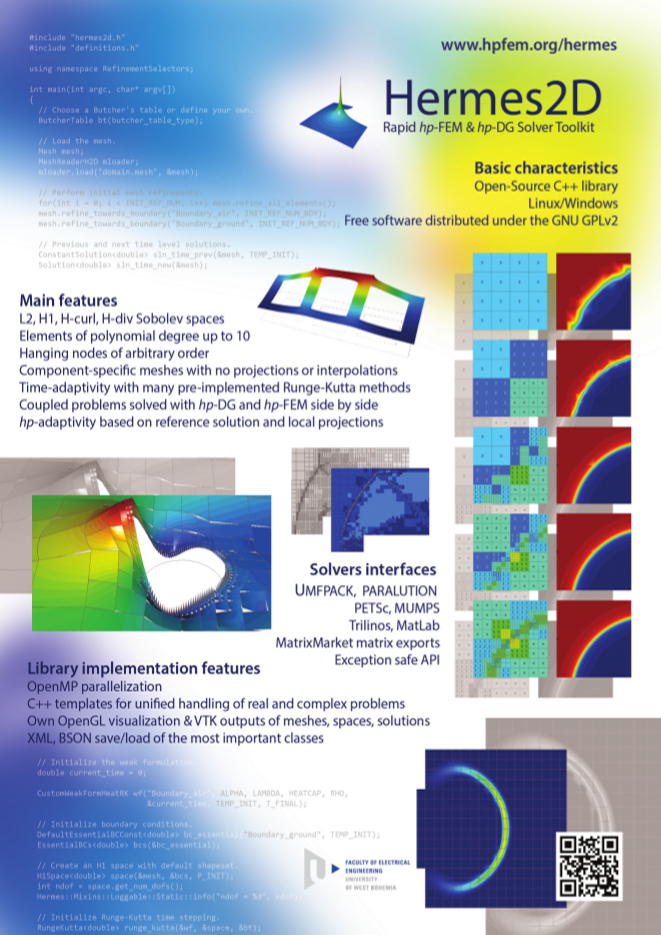
\includegraphics[width=\paperwidth,height=\paperheight, keepaspectratio]{HermesFlyer.jpg}%
\vfill
}}}
\let\origfigure=\figure
\renewenvironment{figure}[6]{
\origfigure[H]}
{\endlist}
\def\degrees{^\circ}
\def\d{{\rm d}}
\pagenumbering{arabic}
\def\L{{\mathcal L}}
\def\H{{\mathcal H}}
\def\M{{\mathcal M}}
\def\matrix{}
\def\fslash#1{#1 \!\!\!/}
\def\F{{\bf F}}
\def\R{{\bf R}}
\def\J{{\bf J}}
\def\x{{\bf x}}
\def\y{{\bf y}}
\def\h{{\rm h}}
\def\a{{\rm a}}
\newcommand{\bfx}{\mbox{\boldmath $x$}}
\newcommand{\bfy}{\mbox{\boldmath $y$}}
\newcommand{\bfz}{\mbox{\boldmath $z$}}
\newcommand{\bfv}{\mbox{\boldmath $v$}}
\newcommand{\bfu}{\mbox{\boldmath $u$}}
\newcommand{\bfF}{\mbox{\boldmath $F$}}
\newcommand{\bfJ}{\mbox{\boldmath $J$}}
\newcommand{\bfU}{\mbox{\boldmath $U$}}
\newcommand{\bfY}{\mbox{\boldmath $Y$}}
\newcommand{\bfR}{\mbox{\boldmath $R$}}
\newcommand{\bfg}{\mbox{\boldmath $g$}}
\newcommand{\bfc}{\mbox{\boldmath $c$}}
\newcommand{\bfxi}{\mbox{\boldmath $\xi$}}
\newcommand{\bfw}{\mbox{\boldmath $w$}}
\newcommand{\bfE}{\mbox{\boldmath $E$}}
\newcommand{\bfS}{\mbox{\boldmath $S$}}
\newcommand{\bfb}{\mbox{\boldmath $b$}}
\newcommand{\bfH}{\mbox{\boldmath $H$}}
\def\Hcurl{{\bfH({\rm curl})}}
\def\Hdiv{{\bfH({\rm div})}}

\newcommand{\dd}[2]{\frac{\partial #1}{\partial #2}}
\newcommand{\dx}{\;\mbox{d}\bfx}


%\def\back{\!\!\!\!\!\!\!\!\!\!}
\def\PY{}
\def\PYZcb{}
\def\PYZob{}
\def\PYZus{}
\def\PYZbs{}
\def\PYZpc{}
\def\PYZti{}
\def\PYZsh{}
\def\PYZhy{-}
\def\back{}
\def\col#1#2{\left(\matrix{#1#2}\right)}
\def\row#1#2{\left(\matrix{#1#2}\right)}
\def\mat#1{\begin{pmatrix}#1\end{pmatrix}}
\def\matd#1#2{\left(\matrix{#1\back0\cr0\back#2}\right)}
\def\p#1#2{{\partial#1\over\partial#2}}
\def\cg#1#2#3#4#5#6{({#1},\,{#2},\,{#3},\,{#4}\,|\,{#5},\,{#6})}
\def\half{{\textstyle{1\over2}}}
\def\jsym#1#2#3#4#5#6{\left\{\matrix{
{#1}{#2}{#3}
{#4}{#5}{#6}
}\right\}}
\def\diag{\hbox{diag}}

\font\dsrom=dsrom10
\def\one{\hbox{\dsrom 1}}

\def\res{\mathop{\mathrm{Res}}}

\def\mathnot#1{\text{"$#1$"}}


%See Character Table for cmmib10:
%http://www.math.union.edu/~dpvc/jsmath/download/extra-fonts/cmmib10/cmmib10.html
\font\mib=cmmib10
\def\balpha{\hbox{\mib\char"0B}}
\def\bbeta{\hbox{\mib\char"0C}}
\def\bgamma{\hbox{\mib\char"0D}}
\def\bdelta{\hbox{\mib\char"0E}}
\def\bepsilon{\hbox{\mib\char"0F}}
\def\bzeta{\hbox{\mib\char"10}}
\def\boldeta{\hbox{\mib\char"11}}
\def\btheta{\hbox{\mib\char"12}}
\def\biota{\hbox{\mib\char"13}}
\def\bkappa{\hbox{\mib\char"14}}
\def\blambda{\hbox{\mib\char"15}}
\def\bmu{\hbox{\mib\char"16}}
\def\bnu{\hbox{\mib\char"17}}
\def\bxi{\hbox{\mib\char"18}}
\def\bpi{\hbox{\mib\char"19}}
\def\brho{\hbox{\mib\char"1A}}
\def\bsigma{\hbox{\mib\char"1B}}
\def\btau{\hbox{\mib\char"1C}}
\def\bupsilon{\hbox{\mib\char"1D}}
\def\bphi{\hbox{\mib\char"1E}}
\def\bchi{\hbox{\mib\char"1F}}
\def\bpsi{\hbox{\mib\char"20}}
\def\bomega{\hbox{\mib\char"21}}

\def\bvarepsilon{\hbox{\mib\char"22}}
\def\bvartheta{\hbox{\mib\char"23}}
\def\bvarpi{\hbox{\mib\char"24}}
\def\bvarrho{\hbox{\mib\char"25}}
\def\bvarphi{\hbox{\mib\char"27}}

%how to use:
%$$\alpha\balpha$$
%$$\beta\bbeta$$
%$$\gamma\bgamma$$
%$$\delta\bdelta$$
%$$\epsilon\bepsilon$$
%$$\zeta\bzeta$$
%$$\eta\boldeta$$
%$$\theta\btheta$$
%$$\iota\biota$$
%$$\kappa\bkappa$$
%$$\lambda\blambda$$
%$$\mu\bmu$$
%$$\nu\bnu$$
%$$\xi\bxi$$
%$$\pi\bpi$$
%$$\rho\brho$$
%$$\sigma\bsigma$$
%$$\tau\btau$$
%$$\upsilon\bupsilon$$
%$$\phi\bphi$$
%$$\chi\bchi$$
%$$\psi\bpsi$$
%$$\omega\bomega$$
%
%$$\varepsilon\bvarepsilon$$
%$$\vartheta\bvartheta$$
%$$\varpi\bvarpi$$
%$$\varrho\bvarrho$$
%$$\varphi\bvarphi$$

%small font
\font\mibsmall=cmmib7
\def\bsigmasmall{\hbox{\mibsmall\char"1B}}

\def\Tr{\hbox{Tr}\,}
\def\Arg{\hbox{Arg}}
\def\atan{\hbox{atan}}


\title{Hermes Documentation}
\date{August 03, 2014}
\release{3.1.0}
\author{hp-FEM group}
\newcommand{\sphinxlogo}{}
\renewcommand{\releasename}{Release}
\makeindex

\makeatletter
\def\PYG@reset{\let\PYG@it=\relax \let\PYG@bf=\relax%
    \let\PYG@ul=\relax \let\PYG@tc=\relax%
    \let\PYG@bc=\relax \let\PYG@ff=\relax}
\def\PYG@tok#1{\csname PYG@tok@#1\endcsname}
\def\PYG@toks#1+{\ifx\relax#1\empty\else%
    \PYG@tok{#1}\expandafter\PYG@toks\fi}
\def\PYG@do#1{\PYG@bc{\PYG@tc{\PYG@ul{%
    \PYG@it{\PYG@bf{\PYG@ff{#1}}}}}}}
\def\PYG#1#2{\PYG@reset\PYG@toks#1+\relax+\PYG@do{#2}}

\expandafter\def\csname PYG@tok@gd\endcsname{\def\PYG@tc##1{\textcolor[rgb]{0.63,0.00,0.00}{##1}}}
\expandafter\def\csname PYG@tok@gu\endcsname{\let\PYG@bf=\textbf\def\PYG@tc##1{\textcolor[rgb]{0.50,0.00,0.50}{##1}}}
\expandafter\def\csname PYG@tok@gt\endcsname{\def\PYG@tc##1{\textcolor[rgb]{0.00,0.27,0.87}{##1}}}
\expandafter\def\csname PYG@tok@gs\endcsname{\let\PYG@bf=\textbf}
\expandafter\def\csname PYG@tok@gr\endcsname{\def\PYG@tc##1{\textcolor[rgb]{1.00,0.00,0.00}{##1}}}
\expandafter\def\csname PYG@tok@cm\endcsname{\let\PYG@it=\textit\def\PYG@tc##1{\textcolor[rgb]{0.25,0.50,0.56}{##1}}}
\expandafter\def\csname PYG@tok@vg\endcsname{\def\PYG@tc##1{\textcolor[rgb]{0.73,0.38,0.84}{##1}}}
\expandafter\def\csname PYG@tok@m\endcsname{\def\PYG@tc##1{\textcolor[rgb]{0.13,0.50,0.31}{##1}}}
\expandafter\def\csname PYG@tok@mh\endcsname{\def\PYG@tc##1{\textcolor[rgb]{0.13,0.50,0.31}{##1}}}
\expandafter\def\csname PYG@tok@cs\endcsname{\def\PYG@tc##1{\textcolor[rgb]{0.25,0.50,0.56}{##1}}\def\PYG@bc##1{\setlength{\fboxsep}{0pt}\colorbox[rgb]{1.00,0.94,0.94}{\strut ##1}}}
\expandafter\def\csname PYG@tok@ge\endcsname{\let\PYG@it=\textit}
\expandafter\def\csname PYG@tok@vc\endcsname{\def\PYG@tc##1{\textcolor[rgb]{0.73,0.38,0.84}{##1}}}
\expandafter\def\csname PYG@tok@il\endcsname{\def\PYG@tc##1{\textcolor[rgb]{0.13,0.50,0.31}{##1}}}
\expandafter\def\csname PYG@tok@go\endcsname{\def\PYG@tc##1{\textcolor[rgb]{0.20,0.20,0.20}{##1}}}
\expandafter\def\csname PYG@tok@cp\endcsname{\def\PYG@tc##1{\textcolor[rgb]{0.00,0.44,0.13}{##1}}}
\expandafter\def\csname PYG@tok@gi\endcsname{\def\PYG@tc##1{\textcolor[rgb]{0.00,0.63,0.00}{##1}}}
\expandafter\def\csname PYG@tok@gh\endcsname{\let\PYG@bf=\textbf\def\PYG@tc##1{\textcolor[rgb]{0.00,0.00,0.50}{##1}}}
\expandafter\def\csname PYG@tok@ni\endcsname{\let\PYG@bf=\textbf\def\PYG@tc##1{\textcolor[rgb]{0.84,0.33,0.22}{##1}}}
\expandafter\def\csname PYG@tok@nl\endcsname{\let\PYG@bf=\textbf\def\PYG@tc##1{\textcolor[rgb]{0.00,0.13,0.44}{##1}}}
\expandafter\def\csname PYG@tok@nn\endcsname{\let\PYG@bf=\textbf\def\PYG@tc##1{\textcolor[rgb]{0.05,0.52,0.71}{##1}}}
\expandafter\def\csname PYG@tok@no\endcsname{\def\PYG@tc##1{\textcolor[rgb]{0.38,0.68,0.84}{##1}}}
\expandafter\def\csname PYG@tok@na\endcsname{\def\PYG@tc##1{\textcolor[rgb]{0.25,0.44,0.63}{##1}}}
\expandafter\def\csname PYG@tok@nb\endcsname{\def\PYG@tc##1{\textcolor[rgb]{0.00,0.44,0.13}{##1}}}
\expandafter\def\csname PYG@tok@nc\endcsname{\let\PYG@bf=\textbf\def\PYG@tc##1{\textcolor[rgb]{0.05,0.52,0.71}{##1}}}
\expandafter\def\csname PYG@tok@nd\endcsname{\let\PYG@bf=\textbf\def\PYG@tc##1{\textcolor[rgb]{0.33,0.33,0.33}{##1}}}
\expandafter\def\csname PYG@tok@ne\endcsname{\def\PYG@tc##1{\textcolor[rgb]{0.00,0.44,0.13}{##1}}}
\expandafter\def\csname PYG@tok@nf\endcsname{\def\PYG@tc##1{\textcolor[rgb]{0.02,0.16,0.49}{##1}}}
\expandafter\def\csname PYG@tok@si\endcsname{\let\PYG@it=\textit\def\PYG@tc##1{\textcolor[rgb]{0.44,0.63,0.82}{##1}}}
\expandafter\def\csname PYG@tok@s2\endcsname{\def\PYG@tc##1{\textcolor[rgb]{0.25,0.44,0.63}{##1}}}
\expandafter\def\csname PYG@tok@vi\endcsname{\def\PYG@tc##1{\textcolor[rgb]{0.73,0.38,0.84}{##1}}}
\expandafter\def\csname PYG@tok@nt\endcsname{\let\PYG@bf=\textbf\def\PYG@tc##1{\textcolor[rgb]{0.02,0.16,0.45}{##1}}}
\expandafter\def\csname PYG@tok@nv\endcsname{\def\PYG@tc##1{\textcolor[rgb]{0.73,0.38,0.84}{##1}}}
\expandafter\def\csname PYG@tok@s1\endcsname{\def\PYG@tc##1{\textcolor[rgb]{0.25,0.44,0.63}{##1}}}
\expandafter\def\csname PYG@tok@gp\endcsname{\let\PYG@bf=\textbf\def\PYG@tc##1{\textcolor[rgb]{0.78,0.36,0.04}{##1}}}
\expandafter\def\csname PYG@tok@sh\endcsname{\def\PYG@tc##1{\textcolor[rgb]{0.25,0.44,0.63}{##1}}}
\expandafter\def\csname PYG@tok@ow\endcsname{\let\PYG@bf=\textbf\def\PYG@tc##1{\textcolor[rgb]{0.00,0.44,0.13}{##1}}}
\expandafter\def\csname PYG@tok@sx\endcsname{\def\PYG@tc##1{\textcolor[rgb]{0.78,0.36,0.04}{##1}}}
\expandafter\def\csname PYG@tok@bp\endcsname{\def\PYG@tc##1{\textcolor[rgb]{0.00,0.44,0.13}{##1}}}
\expandafter\def\csname PYG@tok@c1\endcsname{\let\PYG@it=\textit\def\PYG@tc##1{\textcolor[rgb]{0.25,0.50,0.56}{##1}}}
\expandafter\def\csname PYG@tok@kc\endcsname{\let\PYG@bf=\textbf\def\PYG@tc##1{\textcolor[rgb]{0.00,0.44,0.13}{##1}}}
\expandafter\def\csname PYG@tok@c\endcsname{\let\PYG@it=\textit\def\PYG@tc##1{\textcolor[rgb]{0.25,0.50,0.56}{##1}}}
\expandafter\def\csname PYG@tok@mf\endcsname{\def\PYG@tc##1{\textcolor[rgb]{0.13,0.50,0.31}{##1}}}
\expandafter\def\csname PYG@tok@err\endcsname{\def\PYG@bc##1{\setlength{\fboxsep}{0pt}\fcolorbox[rgb]{1.00,0.00,0.00}{1,1,1}{\strut ##1}}}
\expandafter\def\csname PYG@tok@kd\endcsname{\let\PYG@bf=\textbf\def\PYG@tc##1{\textcolor[rgb]{0.00,0.44,0.13}{##1}}}
\expandafter\def\csname PYG@tok@ss\endcsname{\def\PYG@tc##1{\textcolor[rgb]{0.32,0.47,0.09}{##1}}}
\expandafter\def\csname PYG@tok@sr\endcsname{\def\PYG@tc##1{\textcolor[rgb]{0.14,0.33,0.53}{##1}}}
\expandafter\def\csname PYG@tok@mo\endcsname{\def\PYG@tc##1{\textcolor[rgb]{0.13,0.50,0.31}{##1}}}
\expandafter\def\csname PYG@tok@mi\endcsname{\def\PYG@tc##1{\textcolor[rgb]{0.13,0.50,0.31}{##1}}}
\expandafter\def\csname PYG@tok@kn\endcsname{\let\PYG@bf=\textbf\def\PYG@tc##1{\textcolor[rgb]{0.00,0.44,0.13}{##1}}}
\expandafter\def\csname PYG@tok@o\endcsname{\def\PYG@tc##1{\textcolor[rgb]{0.40,0.40,0.40}{##1}}}
\expandafter\def\csname PYG@tok@kr\endcsname{\let\PYG@bf=\textbf\def\PYG@tc##1{\textcolor[rgb]{0.00,0.44,0.13}{##1}}}
\expandafter\def\csname PYG@tok@s\endcsname{\def\PYG@tc##1{\textcolor[rgb]{0.25,0.44,0.63}{##1}}}
\expandafter\def\csname PYG@tok@kp\endcsname{\def\PYG@tc##1{\textcolor[rgb]{0.00,0.44,0.13}{##1}}}
\expandafter\def\csname PYG@tok@w\endcsname{\def\PYG@tc##1{\textcolor[rgb]{0.73,0.73,0.73}{##1}}}
\expandafter\def\csname PYG@tok@kt\endcsname{\def\PYG@tc##1{\textcolor[rgb]{0.56,0.13,0.00}{##1}}}
\expandafter\def\csname PYG@tok@sc\endcsname{\def\PYG@tc##1{\textcolor[rgb]{0.25,0.44,0.63}{##1}}}
\expandafter\def\csname PYG@tok@sb\endcsname{\def\PYG@tc##1{\textcolor[rgb]{0.25,0.44,0.63}{##1}}}
\expandafter\def\csname PYG@tok@k\endcsname{\let\PYG@bf=\textbf\def\PYG@tc##1{\textcolor[rgb]{0.00,0.44,0.13}{##1}}}
\expandafter\def\csname PYG@tok@se\endcsname{\let\PYG@bf=\textbf\def\PYG@tc##1{\textcolor[rgb]{0.25,0.44,0.63}{##1}}}
\expandafter\def\csname PYG@tok@sd\endcsname{\let\PYG@it=\textit\def\PYG@tc##1{\textcolor[rgb]{0.25,0.44,0.63}{##1}}}

\def\PYGZbs{\char`\\}
\def\PYGZus{\char`\_}
\def\PYGZob{\char`\{}
\def\PYGZcb{\char`\}}
\def\PYGZca{\char`\^}
\def\PYGZam{\char`\&}
\def\PYGZlt{\char`\<}
\def\PYGZgt{\char`\>}
\def\PYGZsh{\char`\#}
\def\PYGZpc{\char`\%}
\def\PYGZdl{\char`\$}
\def\PYGZhy{\char`\-}
\def\PYGZsq{\char`\'}
\def\PYGZdq{\char`\"}
\def\PYGZti{\char`\~}
% for compatibility with earlier versions
\def\PYGZat{@}
\def\PYGZlb{[}
\def\PYGZrb{]}
\makeatother

\begin{document}
\AddToShipoutPicture*{\BackgroundPic}
\ \\ \newpage
\ClearShipoutPicture
\maketitle
\tableofcontents
\phantomsection\label{index::doc}

\chapter{Introduction}
\label{src/introduction:introduction}\label{src/introduction::doc}\label{src/introduction:hermes}

\section{Introduction}
\label{src/intro:introduction}\label{src/intro::doc}\floatplacement{figure}{H}
Thank you for your interest in Hermes!

Hermes is a C++ library for rapid development of adaptive \emph{hp}-FEM and \emph{hp}-DG solvers,
with emphasis on nonlinear, time-dependent, multi-physics problems.

This document is organized as follows:
\begin{itemize}
\item {} 
Section 1 provides general information about Hermes and the computational methods it uses,
and how to install Hermes on various platforms.

\item {} 
Section 2 is the Getting Started Guide - to get you started in no time.

\item {} 
Section 3 is the extended documentation section, you will find developers documentation in Doxygen,
as well as step-by-step user documentation in tutorials and advanced examples.

\item {} 
Section 4 explains how to use Git and Github, and how you can contribute to the project if interested.

\end{itemize}

This document is under continuous development. If you find bugs, typos, dead links
and such, please report them to the
\href{http://groups.google.com/group/hermes2d/}{Hermes2D mailing list}.


\chapter{Hermes Overview}
\label{src/introduction1::doc}\label{src/introduction1:hermes-overview}

\section{About Hermes}
\label{src/about-hermes::doc}\label{src/about-hermes:about-hermes}
Hermes is a free C++ library for rapid development of
adaptive \emph{hp}-FEM and \emph{hp}-DG solvers for partial differential equations (PDE)
and multiphysics PDE systems. The development team now includes mostly the department of Theory of Electrical Engineering at the University of West Bohemia in Pilsen (contact: \href{mailto:korous@rice.zcu.cz}{korous@rice.zcu.cz}), in the past the main development was done by the \href{http://hpfem.org/hermes}{hp-FEM group} at the \href{http://www.unr.edu}{University of Nevada, Reno}.
Information about further collaborators from numerous places around the globe can be found at \href{http://www.hpfem.org/citing/}{http://www.hpfem.org/citing/}.

A standard way to use Hermes is to write short C++ user programs
that use the functionality provided by the library, but for
those who prefer to use a graphical interface, the group located at the
University of West Bohemia also develops a graphical Engineering tool based on Hermes2D:
\href{http://agros2d.org/}{Agros2D}.
\begin{figure}[htbp]
\centering

\scalebox{0.500000}{\includegraphics{agros.png}}
\end{figure}

Hermes is loaded with modern finite element technology. We hope that you will enjoy
the software and that you will find this documentation useful.
In any case please let us know if you find mistakes
or if you can suggest improvements to this documentation or to Hermes itself.

Free use of this software is granted under the terms of the GNU Lesser General
Public License (LGPL). For details see the files \emph{COPYING} and \emph{COPYING.LESSER}.


\section{Mathematical Background}
\label{src/math-background:mathematical-background}\label{src/math-background::doc}
The main strength of Hermes is a modern adaptive higher-order
finite element technology combined with very easy-to-use implementation approaches.


\subsection{Features}
\label{src/math-background:features}\begin{itemize}
\item {} 
Curvilinear elements.

\item {} 
Reduced mesh generation needs.

\item {} 
Arbitrary-level hanging nodes.

\item {} 
Scalar and vector-valued approximations.

\item {} 
Advanced nonlinear solver capabilities.

\item {} 
Exponential convergence of adaptive \emph{hp}-FEM.

\item {} 
Dozens of time-integration methods.

\item {} 
Adaptivity with dynamical meshes for time-dependent problems.

\item {} 
Adaptive multimesh \emph{hp}-FEM for multiphysics coupled problems.

\item {} 
Coupled problems solved together with hp-DG and hp-FEM.

\item {} 
Calculations with physical quantities defined in different subdomains.

\end{itemize}

Some the above points are discussed in more detail below:
\begin{itemize}
\item {} 
\textbf{Curvilinear elements}: Approximating curved boundaries or material interfaces via small elements with straight edges belongs to history. It is much more efficient to employ curvilinear elements, such as in the following acoustics problem.

\end{itemize}
\begin{figure}[htbp]
\centering

\scalebox{0.700000}{\includegraphics{acoustic.png}}
\end{figure}
\begin{itemize}
\item {} 
\textbf{Reduced mesh generation needs}: The previous result was obtained with the mesh shown below, but we also provide support for traditional mesh generators including Triangle, CUBIT, GMSH.

\end{itemize}
\begin{figure}[htbp]
\centering

\scalebox{0.400000}{\includegraphics{initmesh.png}}
\end{figure}
\begin{itemize}
\item {} 
\textbf{Arbitrary-level hanging nodes}: Hermes can handle irregular meshes with arbitrary-level hanging nodes. This makes adaptive algorithms much faster compared to algorithms that use regular meshes (without hanging nodes).

\end{itemize}
\begin{figure}[htbp]
\centering

\scalebox{0.500000}{\includegraphics{ord_2d_c.png}}
\end{figure}
\begin{itemize}
\item {} 
\textbf{Exponential convergence of adaptive hp-FEM}: Many practitioners are skeptical about adaptive FEM because it makes computations slow. However, the exponential convergence of adaptive \emph{hp}-FEM is very different from slow, algebraic convergence of standard low-order FEM. A typical comparison of adaptive low-order FEM and \emph{hp}-FEM is shown below. Here \emph{p=1} and \emph{p=2} means linear and quadratic elements, respectively. The vertical axis shows the approximation error, the horizontal one the number of degrees of freedom (problem size).

\end{itemize}
\begin{figure}[htbp]
\centering

\scalebox{0.500000}{\includegraphics{conv_dof.png}}
\end{figure}

Same graphs as above but now in terms of CPU time:
\begin{figure}[htbp]
\centering

\scalebox{0.500000}{\includegraphics{conv_cpu.png}}
\end{figure}
\begin{itemize}
\item {} 
\textbf{Dozens of time-integration methods}: Hermes has a unique way of using time-integration methods. More than 30 methods are readily available, including the most advanced adaptive implicit higher-order methods. The sample results below illustrate that it is highly recommended to take the time-discretization error seriously (below on the left). The reason is that it can easily be orders of magnitude larger than the error in space (below on the right).

\end{itemize}
\begin{figure}[htbp]
\centering

\scalebox{0.700000}{\includegraphics{time_error.png}}
\end{figure}
\begin{itemize}
\item {} 
\textbf{Multimesh hp-FEM}: Approximating different physical fields on the same mesh belongs to history. For a given solution component, just one finite element mesh can be optimal. Hermes uses an original adaptive multimesh \emph{hp}-FEM technology to discretize any multiphysics problem \emph{on multiple meshes in a monolithic fashion}. No error due to data transfer between various meshes is present. The following figure illustrates this on a coupled problem of heat and moisture transfer in massive concrete walls of a nuclear reactor vessel.

\end{itemize}
\begin{figure}[htbp]
\centering

\scalebox{0.500000}{\includegraphics{hm-sln-frame.png}}
\end{figure}
\begin{figure}[htbp]
\centering

\scalebox{0.500000}{\includegraphics{hm-mesh-frame.png}}
\end{figure}
\begin{itemize}
\item {} 
\textbf{Dynamical meshes for time-dependent problems}: In time-dependent problems, different physical fields or solution components can be approximated on individual meshes that evolve in time independently of each other.

\end{itemize}
\begin{figure}[htbp]
\centering

\scalebox{0.700000}{\includegraphics{flame.jpg}}
\end{figure}
\begin{itemize}
\item {} 
\textbf{Wide applicability}: Hermes does not employ any error estimate or another technique that would limit its applicability to some particular class of PDE problems. It allows you to tackle an arbitrary PDE or multiphysics PDE system. Visit the \href{http://hpfem.org/}{hp-FEM group home page} and the \href{http://hpfem.org/gallery/}{gallery} to see examples.

\end{itemize}
\begin{figure}[htbp]
\centering

\scalebox{0.500000}{\includegraphics{ns.jpg}}
\end{figure}


\subsection{Implementation point of view}
\label{src/math-background:implementation-point-of-view}\begin{itemize}
\item {} 
OpenMP parallelization

\item {} 
C++ templates for unified handling of real and complex problems

\item {} 
Own OpenGL visualization \& VTK outputs of meshes, spaces, solutions

\item {} 
User-friendly written easy-to-grasp code

\item {} 
XML, BSON save / load of the most important classes

\item {} 
Solvers interfaces: UMFPACK, PARALUTION, PETSc, MUMPS, …

\item {} 
GMSH, ExodusII mesh formats

\item {} 
Matlab, MatrixMarket matrix exports

\item {} 
Well arranged doxygen documentation

\item {} 
Exception safe API

\end{itemize}


\subsection{Presentation about Hermes given at ESCO 2014 conference}
\label{src/math-background:presentation-about-hermes-given-at-esco-2014-conference}
A number of presentations about Hermes have been given.
\begin{figure}[htbp]
\centering

\scalebox{0.700000}{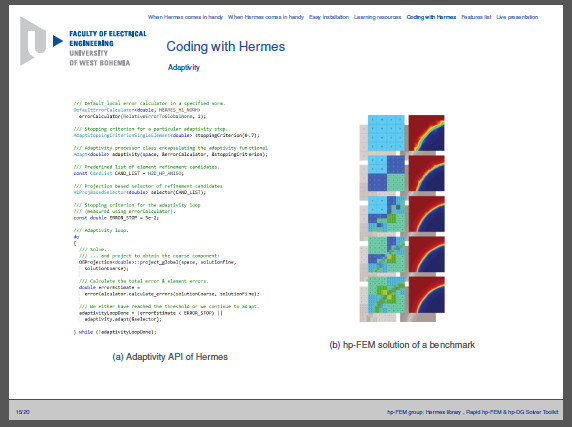
\includegraphics{presentation.jpg}}
\end{figure}

Here is a link to one of them: \href{https://github.com/hpfem/hermes/tree/master-3.1/doc/HermesPresentation.pdf}{https://github.com/hpfem/hermes/tree/master-3.1/doc/HermesPresentation.pdf}.


\section{Citing Hermes}
\label{src/citing-hermes::doc}\label{src/citing-hermes:citing-hermes}
If you use Hermes for your work, please be so kind to include some of the references below as appropriate.

\textbf{Monographs}:

\begin{Verbatim}[commandchars=\\\{\}]
@Book\PYGZob{}Hermes\PYGZhy{}book1,
   author = \PYGZob{}P. Solin, K. Segeth, I. Dolezel\PYGZcb{},
   title = \PYGZob{}Higher\PYGZhy{}Order Finite Element Methods\PYGZcb{},
   publisher = \PYGZob{}Chapman \PYGZam{} Hall / CRC Press\PYGZcb{},
   year = \PYGZob{}2003\PYGZcb{}
\PYGZcb{}
\end{Verbatim}

\begin{Verbatim}[commandchars=\\\{\}]
@Book\PYGZob{}Hermes\PYGZhy{}book2,
   author = \PYGZob{}P. Solin\PYGZcb{},
   title = \PYGZob{}Partial Differential Equations and the Finite Element Method\PYGZcb{},
   publisher = \PYGZob{}J. Wiley \PYGZam{} Sons\PYGZcb{},
   year = \PYGZob{}2005\PYGZcb{}
\PYGZcb{}
\end{Verbatim}

\textbf{Reference to the Hermes open-source project}:

\begin{Verbatim}[commandchars=\\\{\}]
@Manual\PYGZob{}Hermes\PYGZhy{}project,
   title =  \PYGZob{}Hermes \PYGZhy{} Higher\PYGZhy{}Order Modular Finite Element System (User\PYGZsq{}s Guide)\PYGZcb{},
   author = \PYGZob{}P. Solin et al.\PYGZcb{},
   url =    \PYGZob{}http://hpfem.org/\PYGZcb{}
\PYGZcb{}
\end{Verbatim}

\textbf{Underlying algorithms (hanging nodes, adaptivity, shape functions)}:
\begin{Verbatim}[commandchars=\\\{\}]
@Article\PYZob{}Hermes\PYZhy{}time\PYZhy{}integration,
  author = \PYZob{}P. Solin, L. Korous\PYZcb{},
  title = \PYZob{}Adaptive Higher\PYZhy{}Order Finite Element Methods for Transient PDE
  Problems Based on Embedded Higher\PYZhy{}Order Implicit Runge\PYZhy{}Kutta Methods\PYZcb{},
  journal = \PYZob{}J. Comput. Physics\PYZcb{},
  year = \PYZob{}2011\PYZcb{},
  status = \PYZob{}accepted\PYZcb{},
  volume = \PYZob{}\PYZcb{},
  pages = \PYZob{}\PYZcb{}
\PYZcb{}
\end{Verbatim}
\begin{Verbatim}[commandchars=\\\{\}]
@Article\PYZob{}Hermes\PYZhy{}hanging\PYZhy{}nodes,
  author = \PYZob{}P. Solin, J. Cerveny, I. Dolezel\PYZcb{},
  title = \PYZob{}Arbitrary\PYZhy{}Level Hanging Nodes and Automatic Adaptivity
  in the hp\PYZhy{}FEM\PYZcb{},
  journal = \PYZob{}Math. Comput. Simul.\PYZcb{},
  year = \PYZob{}2008\PYZcb{},
  volume = \PYZob{}77\PYZcb{},
  pages = \PYZob{}117 \PYZhy{} 132\PYZcb{}
\PYZcb{}
\end{Verbatim}
\begin{Verbatim}[commandchars=\\\{\}]
@Article\PYZob{}Hermes\PYZhy{}adaptivity,
  author = \PYZob{}P. Solin, D. Andrs, J. Cerveny, M. Simko\PYZcb{},
  title = \PYZob{}PDE\PYZhy{}Independent Adaptive hp\PYZhy{}FEM Based on Hierarchic Extension of
  Finite Element Spaces\PYZcb{},
  journal = \PYZob{}J. Comput. Appl. Math.\PYZcb{},
  year = \PYZob{}2010\PYZcb{},
  volume = \PYZob{}233\PYZcb{},
  pages = \PYZob{}3086\PYZhy{}3094\PYZcb{}
\PYZcb{}
\end{Verbatim}
\begin{Verbatim}[commandchars=\\\{\}]
@Article\PYZob{}Hermes\PYZhy{}shape\PYZhy{}functions,
  author = \PYZob{}P. Solin, T. Vejchodsky\PYZcb{},
  title = \PYZob{}Higher\PYZhy{}Order Finite Elements Based on Generalized Eigenfunctions of
  the Laplacian\PYZcb{},
  journal = \PYZob{}Int. J. Numer. Methods Engrg\PYZcb{},
  year = \PYZob{}2007\PYZcb{},
  volume = \PYZob{}73\PYZcb{},
  pages = \PYZob{}1374 \PYZhy{} 1394\PYZcb{}
\PYZcb{}
\end{Verbatim}

\textbf{Selected applications}:
\begin{Verbatim}[commandchars=\\\{\}]
 @Article\PYZob{}Hermes\PYZhy{}polymer\PYZhy{}metal\PYZhy{}composites,
   author = \PYZob{}D. Pugal, P. Solin, K.J. Kim, A. Aabloo\PYZcb{},
   title = \PYZob{}Modeling Ionic Polymer\PYZhy{}Metal Composites with Space\PYZhy{}Time
   Adaptive Multimesh hp\PYZhy{}FEM\PYZcb{},
   journal = \PYZob{}Communications in Computational Physics\PYZcb{},
   year = \PYZob{}2011\PYZcb{},
   status = \PYZob{}accepted\PYZcb{},
   volume = \PYZob{}\PYZcb{},
   pages = \PYZob{}\PYZcb{}
 \PYZcb{}
\end{Verbatim}
\begin{Verbatim}[commandchars=\\\{\}]
 @Article\PYZob{}Hermes\PYZhy{}anisotropic\PYZhy{}benchmarks,
   author = \PYZob{}P. Solin, O. Certik, L. Korous\PYZcb{},
   title = \PYZob{}Three Anisotropic Benchmarks for Adaptive Finite Element Methods\PYZcb{},
   journal = \PYZob{}Appl. Math. Comput.\PYZcb{},
   year = \PYZob{}2011\PYZcb{},
   status = \PYZob{}accepted\PYZcb{},
   volume = \PYZob{}\PYZcb{},
   pages = \PYZob{}\PYZcb{}
 \PYZcb{}
\end{Verbatim}
\begin{Verbatim}[commandchars=\\\{\}]
 @Article\PYZob{}Hermes\PYZhy{}richards,
   author = \PYZob{}P. Solin, M. Kuraz\PYZcb{},
   title = \PYZob{}Solving the Nonstationary Richards Equation with Adaptive hp\PYZhy{}FEM\PYZcb{},
   journal = \PYZob{}Advanced Water Resources\PYZcb{},
   year = \PYZob{}2011\PYZcb{},
   volume = \PYZob{}34\PYZcb{},
   pages = \PYZob{}1062\PYZhy{}1081\PYZcb{}
 \PYZcb{}
\end{Verbatim}
\begin{Verbatim}[commandchars=\\\{\}]
 @Article\PYZob{}Hermes\PYZhy{}nuclear,
   author = \PYZob{}L. Dubcova, P. Solin, G. Hansen, H. Park\PYZcb{},
   title = \PYZob{}Comparison of Multimesh hp\PYZhy{}FEM to Interpolation and Projection Methods
   for Spatial Coupling of Reactor Thermal and Neutron Diffusion Calculations\PYZcb{},
   journal = \PYZob{}J. Comput. Physics\PYZcb{},
   year = \PYZob{}2011\PYZcb{},
   volume = \PYZob{}230\PYZcb{},
   pages = \PYZob{}1182\PYZhy{}1197\PYZcb{}
 \PYZcb{}
\end{Verbatim}
\begin{Verbatim}[commandchars=\\\{\}]
@Article\PYZob{}Hermes\PYZhy{}heat\PYZhy{}and\PYZhy{}moisture,
  author = \PYZob{}P. Solin, L. Dubcova, J. Kruis,
  title = \PYZob{}Adaptive hp\PYZhy{}FEM with Dynamical Meshes for Transient Heat and Moisture
  Transfer Problems\PYZcb{},
  journal = \PYZob{}J. Comput. Appl. Math\PYZcb{},
  year = \PYZob{}2010\PYZcb{},
  volume = \PYZob{}233\PYZcb{},
  pages = \PYZob{}3103\PYZhy{}3112\PYZcb{}
\PYZcb{}
\end{Verbatim}
\begin{Verbatim}[commandchars=\\\{\}]
@Article\PYZob{}Hermes\PYZhy{}thermoelasticity,
  author = \PYZob{}P. Solin, J. Cerveny, L. Dubcova, D. Andrs\PYZcb{},
  title = \PYZob{}Monolithic Discretization of Linear Thermoelasticity Problems via
  Adaptive Multimesh hp\PYZhy{}FEM\PYZcb{},
  journal = \PYZob{}J. Comput. Appl. Math\PYZcb{},
  status = \PYZob{}published online\PYZcb{},
  doi = \PYZob{}doi 10.1016/j.cam.2009.08.092\PYZcb{},
  year = \PYZob{}2009\PYZcb{}
\PYZcb{}
\end{Verbatim}
\begin{Verbatim}[commandchars=\\\{\}]
@Article\PYZob{}Hermes\PYZhy{}electromagnetics,
  author = \PYZob{}L. Dubcova, P. Solin, J. Cerveny, P. Kus\PYZcb{},
  title = \PYZob{}Space and Time Adaptive Two\PYZhy{}Mesh hp\PYZhy{}FEM for Transient Microwave Heating
  Problems\PYZcb{},
  journal = \PYZob{}Electromagnetics\PYZcb{},
  year = \PYZob{}2010\PYZcb{},
  volume = \PYZob{}30\PYZcb{},
  pages = \PYZob{}23 \PYZhy{} 40\PYZcb{}
\PYZcb{}
\end{Verbatim}
\begin{Verbatim}[commandchars=\\\{\}]
@Article\PYZob{}Hermes\PYZhy{}fluid\PYZhy{}mechanics,
  author = \PYZob{}P. Solin, J. Cerveny, L. Dubcova, I. Dolezel\PYZcb{},
  title = \PYZob{}Multi\PYZhy{}Mesh hp\PYZhy{}FEM for Thermally Conductive Incompressible Flow\PYZcb{},
  journal = \PYZob{}Proceedings of ECCOMAS Conference COUPLED PROBLEMS 2007 (M. Papadrakakis,
  E. Onate, B. Schrefler Eds.), CIMNE, Barcelona\PYZcb{},
  year = \PYZob{}2007\PYZcb{},
  pages = \PYZob{}677 \PYZhy{} 680\PYZcb{}
\PYZcb{}
\end{Verbatim}

Other papers that may be still closer to what you need can be found in the \href{http://www.hpfem.org/citing/}{citing section} of the hp-FEM group home page.


\chapter{Installation}
\label{src/installation:installation}\label{src/installation::doc}

\section{Linux}
\label{src/installation/linux::doc}\label{src/installation/linux:linux}

\subsection{Download and compilation}
\label{src/installation/linux:download-and-compilation}\begin{figure}[htbp]
\centering

\scalebox{1.000000}{
\includegraphics{redRow.jpg}}
\end{figure}

\begin{notice}{note}{{[}NEW{]} - debian packages on Launchpad}

You can download a package directly from \href{https://launchpad.net/~lukas-korous/+archive/ubuntu/hermes}{https://launchpad.net/\textasciitilde{}lukas-korous/+archive/ubuntu/hermes}.
\end{notice}
\begin{figure}[htbp]
\centering

\scalebox{1.000000}{
\includegraphics{redRow.jpg}}
\end{figure}

The rest of the instructions here are for building Hermes from source.

If you are using a Debian-based system, install the (required) libraries first:

If you want to use fast saving / loading of Hermes entities, install
\begin{itemize}
\item {} 
BSON
\begin{itemize}
\item {} 
Clone the BSON Mongo driver git repository from \href{mailto:git@github.com}{git@github.com}:l-korous/mongo-c-driver.git (if you don't know how, here is a tip: \href{http://git-scm.com/book/en/Git-Basics-Getting-a-Git-Repository}{Getting a Git Repository})

\item {} 
Compile and install using `make install'

\end{itemize}

\end{itemize}

For thread caching memory allocator from Google, see
\begin{itemize}
\item {} 
TCMalloc
\begin{itemize}
\item {} 
Get TCMalloc from the SVN repository at \href{http://code.google.com/p/gperftools/source/checkout}{http://code.google.com/p/gperftools/source/checkout}.

\item {} 
Make \& install

\end{itemize}

\end{itemize}

To obtain the source code, clone the Git repository from Github:

\begin{Verbatim}[commandchars=\\\{\}]
\PYG{n}{git} \PYG{n}{clone} \PYG{n}{git}\PYG{o}{:}\PYG{c+c1}{//github.com/hpfem/hermes.git}
\end{Verbatim}

These two repositories are synchronized. For more advanced users we recommend to
create a free account at \href{http://github.com}{Github} (if you do not have one yet),
fork the \href{http://github.com/hpfem/hermes}{Hermes repository}, and then clone your
Github copy of Hermes to your local computer. This will establish links between
your local copy and the master repository, and you'll become part of the Hermes
network at Github.

Once you have a local copy of the Hermes repository on your computer, change dir
to hermes/. There you will find a CMake.vars.example.Linux file that looks like this:

\begin{Verbatim}[commandchars=\\\{\}]
\PYGZsh{} LINUX
  \PYGZsh{} On linux, there should be no need to set up *\PYGZus{}ROOT directories, in the default settings, they all point to /usr/local, as should be true on Debian systems.
  \PYGZsh{} We mainly support gcc and CLang compilers with C++11 support.

  \PYGZsh{} BASIC CONFIGURATION

  \PYGZsh{} Global
\PYGZsh{} Generate static libs (instead of dynamic)
  set(HERMES\PYGZus{}STATIC\PYGZus{}LIBS NO)
  \PYGZsh{} Target path
  set(CMAKE\PYGZus{}INSTALL\PYGZus{}PREFIX \PYGZdq{}/usr/local\PYGZdq{})

  \PYGZsh{} Paths for compulsory dependencies
  set(XERCES\PYGZus{}ROOT \PYGZdq{}/usr/local\PYGZdq{})
  set(XSD\PYGZus{}ROOT \PYGZdq{}/usr/local\PYGZdq{})

  \PYGZsh{} HermesCommon

    \PYGZsh{} Release and debug versions
    set(HERMES\PYGZus{}COMMON\PYGZus{}DEBUG     YES)
    set(HERMES\PYGZus{}COMMON\PYGZus{}RELEASE   YES)
    ...
\end{Verbatim}

Copy this file to ``CMake.vars'' and set the variables according to your needs.
After that, type:

\begin{Verbatim}[commandchars=\\\{\}]
\PYG{n}{cmake} \PYG{p}{.}
\PYG{n}{make}
\end{Verbatim}

If you have more than one CPU, you can use ``make -jN'' where N is
the number of CPUs of your computer.


\subsection{Debugging with Eclipse}
\label{src/installation/linux:debugging-with-eclipse}
To use eclipse as debugger, in the root folder of the project:

\begin{Verbatim}[commandchars=\\\{\}]
\PYG{n}{mkdir} \PYG{n}{eclipse\PYGZus{}build}
\PYG{n}{cd} \PYG{n}{eclipse\PYGZus{}build}
\PYG{n}{cmake} \PYG{o}{\PYGZhy{}}\PYG{n}{G}\PYG{l+s}{\PYGZdq{}}\PYG{l+s}{Eclipse CDT4 \PYGZhy{} Unix Makefiles}\PYG{l+s}{\PYGZdq{}} \PYG{o}{\PYGZhy{}}\PYG{n}{D} \PYG{n}{CMAKE\PYGZus{}BUILD\PYGZus{}TYPE}\PYG{o}{=}\PYG{n}{Debug} \PYG{p}{.}\PYG{p}{.}\PYG{o}{/}
\end{Verbatim}

In Eclipse:
\begin{itemize}
\item {} 
Import project using Menu File-\textgreater{}Import

\item {} 
Select General-\textgreater{}Existing projects into workspace:

\item {} 
Browse where your build tree is and select the root build tree directory.

\item {} 
Keep ``Copy projects into workspace'' unchecked.

\end{itemize}


\subsection{Install Hermes}
\label{src/installation/linux:install-hermes}
\begin{Verbatim}[commandchars=\\\{\}]
\PYG{n}{make} \PYG{n}{install}
\end{Verbatim}


\section{Windows}
\label{src/installation/win:windows}\label{src/installation/win::doc}

\subsection{Download and compilation}
\label{src/installation/win:download-and-compilation}\begin{figure}[htbp]
\centering

\scalebox{1.000000}{
\includegraphics{redRow.jpg}}
\end{figure}

\begin{notice}{note}{{[}NEW{]} - prebuilt binaries}

You can download both the dependency libraries and header files, as well as Hermes libraries and header files from \href{https://github.com/l-korous/hermes-windows}{https://github.com/l-korous/hermes-windows}.
\end{notice}
\begin{figure}[htbp]
\centering

\scalebox{1.000000}{
\includegraphics{redRow.jpg}}
\end{figure}

The rest of the instructions here are for building Hermes from source.

To obtain the source code, clone the Git repository from Github:

\begin{Verbatim}[commandchars=\\\{\}]
\PYG{n}{git} \PYG{n}{clone} \PYG{n}{git}\PYG{o}{:}\PYG{c+c1}{//github.com/hpfem/hermes.git}
\end{Verbatim}

{[}IMPORTANT{]} As Hermes uses features of C++11 (such as initializer lists, nullptr\_t, etc.), the only Visual Studio family compiler you can use is Visual Studio 2013 (both Express and `Full' versions).


\subsection{Dependency check-list - overview}
\label{src/installation/win:dependency-check-list-overview}\begin{itemize}
\item {} 
You need to install dependent libraries into either common directory, or separate directories. This directory, further called `dependencies' (stands for the particular directory in the case of particular dependency), has to have three subdirectories as follows. The choice of having a single common directory, or separate ones is up to you.
\begin{itemize}
\item {} 
`dependencies'\textbackslash{}include: Header files (*.h) of dependency libraries.

\item {} 
`dependencies'\textbackslash{}lib: Library files (*.lib) of dependency libraries.

\item {} 
`dependencies'\textbackslash{}bin: Binary modules (*.dll) of dependency libraries.

\item {} 
be sure to include a directory `dependecies'\textbackslash{}bin into the `PATH' environment variable (you need to include all of them if you chose to have separate ones for various dependencies).

\end{itemize}

\item {} 
For the 64-bit version, if you want to use it side-by-side to the 32-bit one, you can create a subdirectory `x64' in the `lib' folder where you will be putting the 64-bit dependency libraries.

\end{itemize}


\subsection{Dependency check-list - 32-bit}
\label{src/installation/win:dependency-check-list-32-bit}
This list works for 32-bit version of Hermes. See the section for 64-bit version if that is the one you are interested in.
Please note that e.g. TCMalloc, BSON, UMFPACK are also `optional', but to get the most performance out of Hermes, they are recommended.
\begin{itemize}
\item {} 
CMAKE
\begin{itemize}
\item {} 
Download CMAKE installer(\href{http://www.cmake.org/files/v2.8/cmake-2.8.3-win32-x86.exe}{http://www.cmake.org/files/v2.8/cmake-2.8.3-win32-x86.exe}) and install it.

\end{itemize}

\item {} 
UMFPACK
\begin{itemize}
\item {} 
MinGW used for compiling AMD and UMFPACK: \href{http://sourceforge.net/projects/mingw/}{Download MinGW}.

\item {} 
after installing MinGW, add `your-minGW-installation-directory'/bin to system PATH.

\item {} 
download latest \href{http://www.cise.ufl.edu/research/sparse/SuiteSparse\_config/}{SuiteSparse\_config}, \href{http://www.cise.ufl.edu/research/sparse/amd/}{AMD}, and \href{http://www.cise.ufl.edu/research/sparse/umfpack/}{UMFPACK} to  A SINGLE PARENT DIRECTORY (this requirement is one of UMFPACK).

\item {} 
Add the following lines at the end of file SuiteSparse\_config\textbackslash{}SuiteSparse\_config.mk:
\begin{itemize}
\item {} 
CC = gcc

\item {} 
CXX = gcc

\item {} 
UMFPACK\_CONFIG = -DNBLAS

\item {} 
RANLIB = echo

\item {} 
LIB = -lm

\end{itemize}

\item {} 
Open all files called `Makefile' from all three directories and replace all `;' symbols in them with the Windows equivalent `\&'

\item {} 
Copy SuiteSparse\_config\textbackslash{}SuiteSparse\_config.h to `include' directory

\item {} 
Copy SuiteSparse\_config\textbackslash{}libsuitesparseconfig.a to `lib' directory and change its extension to Windows equivalent `.lib'.

\item {} 
Copy AMD\textbackslash{}Include\textbackslash{}amd.h, AMD\textbackslash{}Include\textbackslash{}amd\_internal.h, and AMD\textbackslash{}Lib\textbackslash{}libamd.a to `include', and `lib' dependecy directories respectively. Change the libamd.a's extension to `.lib'

\item {} 
Copy UMFPACK\textbackslash{}Include\textbackslash{}* to `include'

\item {} 
Copy UMFPACK\textbackslash{}Lib\textbackslash{}libumfpack.a to `lib' directory and change its extension to Windows equivalent `.lib'.

\end{itemize}

\item {} 
XERCES
\begin{itemize}
\item {} 
Download Xerces 3.1.1 source code from \href{http://xerces.apache.org/xerces-c/download.cgi}{http://xerces.apache.org/xerces-c/download.cgi}.

\item {} 
Build using your favorite compiler.

\item {} 
Copy all bin files to `bin' dependencies directory

\item {} 
Copy all header files to `include' dependencies directory

\item {} 
Copy the lib files to `lib' dependencies directory

\end{itemize}

\item {} 
XSD
- Download XSD library from \href{http://www.codesynthesis.com/download/xsd/3.3/windows/i686/xsd-3.3.0-i686-windows.zip}{http://www.codesynthesis.com/download/xsd/3.3/windows/i686/xsd-3.3.0-i686-windows.zip}, instructions how to build the library are available at \href{http://wiki.codesynthesis.com/Using\_XSD\_with\_Microsoft\_Visual\_Studio}{http://wiki.codesynthesis.com/Using\_XSD\_with\_Microsoft\_Visual\_Studio}.
- Copy all bin files to `bin' dependencies directory
- Copy all header files to `include' dependencies directory

\item {} 
OpenGL support (optional)
\begin{itemize}
\item {} 
FREEGLUT
\begin{itemize}
\item {} 
Download freeglut 2.4.0 (\href{http://freeglut.sourceforge.net/}{http://freeglut.sourceforge.net/}) and unpack it.

\item {} 
Open the your\_freeglut\_2.4.0\_root\textbackslash{}freeglut.DSP file in Visual Studio and convert it to a newer format.

\item {} 
Compile Debug or Release version. Debug version is recommended in a case of debugging.

\item {} 
Copy `freeglut.dll', `freeglut.h', and `freeglut.lib' to `bin', `include\textbackslash{}GL', and `lib' dependency directories, respectively/.

\end{itemize}

\item {} 
GLEW
\begin{itemize}
\item {} 
Download glew Win32 precompiled binaries ver.1.5.4 (\href{http://glew.sourceforge.net/}{http://glew.sourceforge.net/}) and unpack it.

\item {} 
Copy `my\_glew\_root\textbackslash{}bin\textbackslash{}glew32.dll', `my\_glew\_root\textbackslash{}include\textbackslash{}GL\textbackslash{}*.h', and `my\_glew\_root\textbackslash{}lib\textbackslash{}glew32.lib' to `bin', `include\textbackslash{}GL', and `lib' dependency directories respectively.

\end{itemize}

\item {} 
PTHREAD(2.9.1)

\item {} 
Download appropriate files (\href{ftp://sourceware.org/pub/pthreads-win32/prebuilt-dll-2-9-1-release/}{ftp://sourceware.org/pub/pthreads-win32/prebuilt-dll-2-9-1-release/}).

\item {} 
Copy `dll\textbackslash{}x86\textbackslash{}pthreadVCE2.dll', `include\textbackslash{}*.h' and `lib\textbackslash{}x86\textbackslash{}pthreadVCE2.lib' to `bin', `include', and `lib' dependecy directories respectively.

\end{itemize}

\item {} 
The rest is optional. If a directive WITH\_BSON is \emph{not} used, this step including all sub-steps can be skipped and you can proceed to ``\textbf{Building Hermes}''.
\begin{itemize}
\item {} 
MATIO (1.5.2)
\begin{itemize}
\item {} 
Download HDF5 \href{http://www.hdfgroup.org/ftp/HDF5/releases/hdf5-1.8.7/obtain5187.html}{http://www.hdfgroup.org/ftp/HDF5/releases/hdf5-1.8.7/obtain5187.html}.

\item {} 
Install HDF5, note the path (you will need it for MATIO)

\item {} 
Download MATIO from \href{http://sourceforge.net/projects/matio/}{http://sourceforge.net/projects/matio/}.

\item {} 
Open the sln file in the folder visual\_studio

\item {} 
Add to the Include Directories under the libmatio project settings the directory where you installed HDF5's headers

\item {} 
Add to the Libraries Directories under the libmatio project settings the directory where you installed HDF5's libs

\item {} 
Add to the linker linking to ``libszip.lib''

\item {} 
(Fix MATIO error) Open the file zconf.h and on the line 287 change \#if 1 to \#if 0.

\item {} 
build, copy visual\_studio/\emph{.h and src/}.h to `include' folder, visual\_studio/Release/libmatio.lib to `lib', visual\_studio/Release/libmatio.dll to `bin' folders.

\end{itemize}

\item {} 
BSON
\begin{itemize}
\item {} 
Clone the BSON Mongo driver git repository from \href{mailto:git@github.com}{git@github.com}:l-korous/mongo-c-driver.git (if you don't know how, here is a tip:\href{http://git-scm.com/book/en/Git-Basics-Getting-a-Git-Repository}{Getting a Git Repository})

\item {} 
Download SCONS build tool from \href{http://sourceforge.net/projects/scons/files/latest/download?source=files}{http://sourceforge.net/projects/scons/files/latest/download?source=files}.

\item {} 
Install SCONS (you need to have PYTHON installed for that), run it (e.g. issuing C:Python27Scriptsscons.bat) in the BSON Mongo driver root directory
\begin{itemize}
\item {} 
Use flags --m32 and --c99 (``C:Python27Scriptsscons.bat --c99 --m32'')

\end{itemize}

\item {} 
Once compiled (should take seconds at most), copy src/bson.h to your `include' dependency directory, bson.lib to `lib', and bson.dll to `bin' directories.

\end{itemize}

\item {} 
TCMalloc
\begin{itemize}
\item {} 
Get TCMalloc from the SVN repository at \href{http://code.google.com/p/gperftools/source/checkout}{http://code.google.com/p/gperftools/source/checkout}.

\item {} 
Open gperftools.sln in your Visual Studio, build the appropriate version (default works fine - just select Debug/Release)

\item {} 
Copy Win32''Release/Debug''libtcmalloc\_minimal.dll to `bin' dependency directory, Win32''Release/Debug''libtcmalloc\_minimal.lib to `lib' dependency directory

\item {} 
Copy the contents of src/google to `include' dependency directory

\end{itemize}

\item {} 
ExodusII
\begin{itemize}
\item {} 
Download sources of version 4.9.3 (\href{http://sourceforge.net/projects/exodusii/}{http://sourceforge.net/projects/exodusii/}) and unpack `exodusii'

\item {} 
Add the following line to the file `my\_exodusii\_root\textbackslash{}CMakeLists.txt' as:

\begin{Verbatim}[commandchars=\\\{\}]
\PYG{n}{PROJECT}\PYG{p}{(}\PYG{n}{Exodusii}\PYG{p}{)}
\PYG{n}{SET}\PYG{p}{(}\PYG{n}{NETCDF\PYGZus{}INCLUDE\PYGZus{}DIR} \PYG{l+s}{\PYGZdq{}}\PYG{l+s}{my\PYGZus{}netcdf\PYGZus{}root/libsrc4}\PYG{l+s}{\PYGZdq{}}\PYG{p}{)}
\PYG{c+cp}{\PYGZsh{}}\PYG{c+cp}{ add this line;}
\end{Verbatim}

be sure to use a slash `/' instead of a backslash `\textbackslash{}'.

\item {} 
Generate MSVC project files using CMAKE in command prompt as:

\begin{Verbatim}[commandchars=\\\{\}]
cmake . \PYGZhy{}G \PYGZdq{}Visual Studio 9 2008\PYGZdq{}    \PYGZsh{} MSVC2008 user
cmake . \PYGZhy{}G \PYGZdq{}Visual Studio 10\PYGZdq{}        \PYGZsh{} MSVC2010 user
\end{Verbatim}

If you have Cygwin installed, make sure that you are using the windows version of cmake.

\item {} 
Open a SLN file `my\_exodusii\_root/ExodusII.sln' in MSVC08/10

\item {} 
Switch to `Release' version

\item {} 
Build a project `exoIIv2c': this will create a LIB file in `my\_exodusii\_root\textbackslash{}cbind\textbackslash{}Release'

\item {} 
Copy `exoIIv2c.lib' to `lib' dependency directory structure

\item {} 
Copy `my\_exodusii\_root\textbackslash{}cbind\textbackslash{}include\textbackslash{}exodusII.h and exodusII\_ext.h' to `include' dependency directory

\end{itemize}

\item {} 
CLAPACK
\begin{itemize}
\item {} 
First, you need to install CLAPACK/CBLAS:

\item {} 
Download the file clapack-3.2.1-CMAKE.tgz from \href{http://www.netlib.org/clapack/}{http://www.netlib.org/clapack/}.

\item {} 
Use cmake to configure and build the debug version of clapack.

\item {} 
Copy `\textbackslash{}clapack-3.2.1-CMAKE\textbackslash{}BLAS\textbackslash{}SRC\textbackslash{}Debug\textbackslash{}blas.lib', `\textbackslash{}clapack-3.2.1-CMAKE\textbackslash{}F2CLIBS\textbackslash{}libf2c\textbackslash{}Debug\textbackslash{}libf2c.lib', and `\textbackslash{}clapack-3.2.1-CMAKE\textbackslash{}SRC\textbackslash{}Debug\textbackslash{}lapack.lib' to `lib' dependency directory.

\item {} 
Copy the contains of `\textbackslash{}clapack-3.2.1-CMAKE\textbackslash{}INCLUDE\textbackslash{}' to `include' dependency directory.

\end{itemize}

\end{itemize}

\end{itemize}


\subsection{Dependency check-list - 64-bit}
\label{src/installation/win:dependency-check-list-64-bit}\begin{quote}

Only the most important dependencies are described here for the 64-bit version. For all others, all you must do is compile the 64-bit version, or get it in any other way and link it to Hermes instead of the 32-bit one.
\begin{itemize}
\item {} 
CMAKE
\begin{itemize}
\item {} 
Download CMAKE installer(\href{http://www.cmake.org/files/v2.8/cmake-2.8.3-win32-x86.exe}{http://www.cmake.org/files/v2.8/cmake-2.8.3-win32-x86.exe}) and install it.

\end{itemize}

\item {} 
PTHREAD(2.9.1)
\begin{itemize}
\item {} 
Download appropriate files (\href{ftp://sourceware.org/pub/pthreads-win32/prebuilt-dll-2-9-1-release/}{ftp://sourceware.org/pub/pthreads-win32/prebuilt-dll-2-9-1-release/}).

\item {} 
Copy `dll\textbackslash{}x64\textbackslash{}pthreadVCE2.dll', `include\textbackslash{}*.h' and `lib\textbackslash{}x64\textbackslash{}pthreadVCE2.lib' to `bin', `include', and `lib' dependecy directories respectively.

\end{itemize}

\item {} 
UMFPACK
\begin{itemize}
\item {} 
MinGW used for compiling AMD and UMFPACK: \href{http://sourceforge.net/projects/mingw/}{Download MinGW}.

\item {} 
Just use 64-bit MinGW and provide the flag ``-m64'', otherwise it is the same as in Win32 version.

\end{itemize}

\item {} 
XERCES
\begin{itemize}
\item {} 
Download Xerces 3.1.1 source code from \href{http://xerces.apache.org/xerces-c/download.cgi}{http://xerces.apache.org/xerces-c/download.cgi}.

\item {} 
Build using your favorite compiler for 64-bit.

\item {} 
Copy all bin files to `bin' dependencies directory

\item {} 
Copy all header files to `include' dependencies directory

\item {} 
Copy the lib files to `lib' dependencies directory

\end{itemize}

\item {} 
XSD
- Download XSD library from \href{http://www.codesynthesis.com/download/xsd/3.3/windows/i686/xsd-3.3.0-i686-windows.zip}{http://www.codesynthesis.com/download/xsd/3.3/windows/i686/xsd-3.3.0-i686-windows.zip}, instructions how to build the library are available at \href{http://wiki.codesynthesis.com/Using\_XSD\_with\_Microsoft\_Visual\_Studio}{http://wiki.codesynthesis.com/Using\_XSD\_with\_Microsoft\_Visual\_Studio}.
- Build the x64 version
- Copy all bin files to `bin' dependencies directory
- Copy all header files to `include' dependencies directory

\item {} 
OpenGL support (optional)
\begin{itemize}
\item {} 
FREEGLUT
\begin{itemize}
\item {} 
Download freeglut 2.4.0 (\href{http://freeglut.sourceforge.net/}{http://freeglut.sourceforge.net/}) and unpack it.

\item {} 
Open the your\_freeglut\_2.4.0\_root\textbackslash{}freeglut.DSP file in Visual Studio and convert it to a newer format.

\item {} 
Compile Debug or Release version (x64 platform). Debug version is recommended in a case of debugging.

\item {} 
Copy `freeglut.dll', `freeglut.h', and `freeglut.lib' to `bin', `include\textbackslash{}GL', and `lib' dependency directories, respectively/.

\end{itemize}

\item {} 
GLEW
\begin{itemize}
\item {} 
Download glew x64 precompiled binaries (\href{http://glew.sourceforge.net/}{http://glew.sourceforge.net/}) and unpack it.

\item {} 
Copy `my\_glew\_root\textbackslash{}bin\textbackslash{}glew32.dll', `my\_glew\_root\textbackslash{}include\textbackslash{}GL\textbackslash{}*.h', and `my\_glew\_root\textbackslash{}lib\textbackslash{}glew32.lib' to `bin', `include\textbackslash{}GL', and `lib' dependency directories respectively.

\end{itemize}

\end{itemize}

\item {} 
The rest is optional. If a directive WITH\_BSON is \emph{not} used, this step including all sub-steps can be skipped and you can proceed to ``\textbf{Building Hermes}''.
\begin{itemize}
\item {} 
MATIO (1.5.2)
\begin{itemize}
\item {} 
Just follow the 32-bit version instructions and download HDF5 for x64, and also when building MATIO, build the x64 version.

\end{itemize}

\item {} 
TCMalloc
\begin{itemize}
\item {} 
Get TCMalloc from the SVN repository at \href{http://code.google.com/p/gperftools/source/checkout}{http://code.google.com/p/gperftools/source/checkout}.

\item {} 
Open gperftools.sln in your Visual Studio, build the appropriate version (default works fine - just select Debug/Release)

\item {} 
Copy x64''Release/Debug''libtcmalloc\_minimal.dll to `bin' dependency directory, x64''Release/Debug''libtcmalloc\_minimal.lib to `lib' dependency directory

\item {} 
Copy the contents of src/google to `include' dependency directory

\end{itemize}

\item {} 
BSON
\begin{itemize}
\item {} 
Clone the BSON Mongo driver git repository from \href{mailto:git@github.com}{git@github.com}:l-korous/mongo-c-driver.git (if you don't know how, here is a tip:\href{http://git-scm.com/book/en/Git-Basics-Getting-a-Git-Repository}{Getting a Git Repository})

\item {} 
Download SCONS build tool from \href{http://sourceforge.net/projects/scons/files/latest/download?source=files}{http://sourceforge.net/projects/scons/files/latest/download?source=files}.

\item {} 
Install SCONS (you need to have PYTHON installed for that), run it (e.g. issuing C:Python27Scriptsscons.bat) in the BSON Mongo driver root directory
\begin{itemize}
\item {} 
Use the flag --c99 (``C:Python27Scriptsscons.bat --c99'')

\end{itemize}

\item {} 
Once compiled (should take seconds at most), copy src/bson.h to your `include' dependency directory, bson.lib to `lib', and bson.dll to `bin' directories.

\end{itemize}

\end{itemize}

\end{itemize}
\end{quote}


\subsection{Building Hermes}
\label{src/installation/win:building-hermes}\begin{quote}

In order to build the library and examples, you need to:
\begin{itemize}
\item {} 
Prepare dependecy libraries, see `Dependency Check-list'.

\item {} 
Copy the file `CMake.vars.example.Windows' to `CMake.vars'. The file contains settings for the project.

\item {} 
In the root Hermes directory, generate project files by running CMAKE from a command prompt:

\begin{Verbatim}[commandchars=\\\{\}]
cmake . \PYGZhy{}G \PYGZdq{}Visual Studio 12\PYGZdq{}      \PYGZsh{} MSVC2013 as the generator
\end{Verbatim}

If you have Cygwin installed, your might have an error ``Could not create named generator Visual Studio 12''. This is because your
cmake path is contaminated by Cygwin's cmake. Try to use absolute path for windows cmake.exe.

\item {} 
Open the SLN file `hermes.sln' and build Hermes.

\end{itemize}
\end{quote}


\subsection{Using Hermes}
\label{src/installation/win:using-hermes}
In order to use Hermes in your project, you need to do the following steps. Steps has 5, 6, and 7 to be repeated for every configuration, i.e., Debug, Release. Except the step 7b, this can be done easily by setting the drop-down Configuration to `All configurations' in the Project Property dialog.
\begin{itemize}
\item {} 
Prepare Hermes to be buildable by MSVC, see `Building Hermes'.

\item {} 
Create your project in MSVC. Set the project to be an empty Win32 console project.

\item {} 
Add directories `dependencies\textbackslash{}lib' to additional library directories (\textless{}right click on your project\textgreater{}\textbackslash{}Properties\textbackslash{}Configuration Properties\textbackslash{}Linker\textbackslash{}Additional Library Directories).

\item {} 
Add also the directory where you copied Hermes libraries to as an additional library directory. This would probably be the variable CMAKE\_INSTALL\_PREFIX in your CMake.vars file.

\item {} 
Add `include ``hermes2d.h''', make sure that your CMAKE\_INSTALL\_PREFIX is among Include Directories settings in your compiler.

\item {} 
Add the dependencies\textbackslash{}include directory (and possibly other directories where you copied dependency headers) using
\begin{itemize}
\item {} 
Project -\textgreater{} Properties -\textgreater{} Configuration Properties -\textgreater{} VC++ Directories -\textgreater{} Include Directories

\end{itemize}

\item {} 
Deny (Ignore) warnings that are not indicating anything dangerous:
\begin{itemize}
\item {} 
Ignore warnings about STL in DLL by denying a warning 4251 (\textless{}right click on your project\textgreater{}\textbackslash{}Properties\textbackslash{}Configuration Properties\textbackslash{}C/C++\textbackslash{}Advanced\textbackslash{}Disable Specific Warnings, enter 4251).

\item {} 
Ignore warnings about standard functions that are not safe (\textless{}right click on your project\textgreater{}\textbackslash{}Properties\textbackslash{}Configuration Properties\textbackslash{}C/C++\textbackslash{}Preprocessor\textbackslash{}Preprocessor Definitions, add \_CRT\_SECURE\_NO\_WARNINGS).

\item {} 
Also ignore any template instantiation warnings

\end{itemize}

\item {} 
Resolve unresolved linker error in Xerces
- \href{http://stackoverflow.com/questions/10506582/xerces-c-unresolved-linker-error}{http://stackoverflow.com/questions/10506582/xerces-c-unresolved-linker-error}

\end{itemize}


\section{Mac OS}
\label{src/installation/mac:mac-os}\label{src/installation/mac::doc}

\subsection{Download and compilation}
\label{src/installation/mac:download-and-compilation}
\textbf{Known issues}: Hermes has built-in OpenGL visualization based on FreeGlut, but this package
comes with certain installation difficulties. If you encounter Glut-related problems, set
H2D\_WITH\_GLUT to NO in Cmake.vars, build Hermes without Glut, and use VTK output for visualization.

\textbf{Step 1}: Make sure you have XCode installed. This should be on the installation
disks which came with your Mac. XCode contains the GNU compilers, make
and many other things which are required to build Hermes.

\textbf{Step 3}: Install the following libraries and applications: Suitesparse,
glew, cmake, git. If you don't already have these on your Mac, then
the easiest way to get them is to use MacPorts (which is an
application which allows you to easily install and manage UNIX
libraries and applications on your Mac) by doing the following:
\begin{enumerate}
\item {} 
Download and install MacPorts from
\href{http://www.macports.org/install.php}{http://www.macports.org/install.php}.

\item {} 
Do `sudo port install suitesparse glew'.

\item {} 
If you don't already have git installed, do
`sudo port install git'.

\item {} 
If you don't already have cmake installed, do
`sudo port install cmake'.

\end{enumerate}

\textbf{Step 4}: Get the Hermes source code as described at the beginning of the Linux section
above. Change to the directory where you want
to download the Hermes source and clone the git repository either
from the hpfem.org server:

\begin{Verbatim}[commandchars=\\\{\}]
git clone {}`\PYGZlt{}http://git.hpfem.org/git/hermes.git\PYGZgt{}{}`\PYGZus{}.
\end{Verbatim}

or from Github:

\begin{Verbatim}[commandchars=\\\{\}]
\PYG{n}{git} \PYG{n}{clone} \PYG{n}{git}\PYG{o}{:}\PYG{c+c1}{//github.com/hpfem/hermes.git}
\end{Verbatim}

These two repositories are synchronized. For more advanced users we recommend
to create a free account at Github (if you do not have one yet), fork the
Hermes repository, and then clone your Github copy of Hermes to your local computer.
This will establish links between your local copy and the master repository, and
you’ll become part of the Hermes network at Github.

\textbf{Step 5}: Configure and build Hermes by changing dir to `hermes/',
and then typing `cmake .' and `make'.
If you have more than one CPU, you can use `make -jN' where N is the
number of CPUs of your computer. To set the location where Hermes
will be installed, pass the -DCMAKE\_INSTALL\_PREFIX=\textless{}your location\textgreater{}
flag to cmake (i.e. to install in /usr/local, replace the cmake
command above with `cmake -DCMAKE\_INSTALL\_PREFIX=/usr/local .').

\textbf{Step 6}: Install Hermes by doing `make install'.


\subsection{More options}
\label{src/installation/mac:more-options}
You can turn on and off various components to build, just create the CMake.vars
file and add the following:

\begin{Verbatim}[commandchars=\\\{\}]
\PYG{n}{set}\PYG{p}{(}\PYG{n}{H2D\PYGZus{}WITH\PYGZus{}GLUT} \PYG{n}{NO}\PYG{p}{)}
\end{Verbatim}

(and any other option that you would like to change, see CMakeLists.txt for the
whole list).

For development, it is good to say (in global CMake.vars):

\begin{Verbatim}[commandchars=\\\{\}]
\PYG{n}{set}\PYG{p}{(}\PYG{n}{DEBUG} \PYG{n}{YES}\PYG{p}{)} \PYG{n}{to} \PYG{n}{compile} \PYG{n}{debug} \PYG{n}{versions}
\PYG{n}{set}\PYG{p}{(}\PYG{n}{RELEASE} \PYG{n}{YES}\PYG{p}{)} \PYG{n}{to} \PYG{n}{compile} \PYG{n}{release} \PYG{n}{versions}
\end{Verbatim}

Then type:

\begin{Verbatim}[commandchars=\\\{\}]
\PYG{n}{make} \PYG{n}{debug}    \PYG{p}{(}\PYG{n}{to} \PYG{n}{build} \PYG{n}{debug} \PYG{n}{versions}\PYG{p}{)}
\PYG{n}{make} \PYG{n}{release}  \PYG{p}{(}\PYG{n}{to} \PYG{n}{build} \PYG{n}{release} \PYG{n}{versions}\PYG{p}{)}
\end{Verbatim}


\section{Installation of Matrix Solvers}
\label{src/installation/matrix_solvers:installation-of-matrix-solvers}\label{src/installation/matrix_solvers::doc}

\subsection{Mumps}
\label{src/installation/matrix_solvers/mumps::doc}\label{src/installation/matrix_solvers/mumps:mumps}

\subsubsection{Linux}
\label{src/installation/matrix_solvers/mumps:linux}\label{src/installation/matrix_solvers/mumps:mumps-home-page}

\paragraph{Using standard Debian packages}
\label{src/installation/matrix_solvers/mumps:using-standard-debian-packages}
For sequential version, install packages \emph{libmumps-seq-4.9.2} and \emph{libmumps-seq-dev}.
For parallel version, install \emph{libmumps-4.9.2} and \emph{libmumps-dev}. Newer versions
may be available. In Ubuntu 6.06 (Dapper)
or newer, you can use the Synaptic package manager for that, or type:

\begin{Verbatim}[commandchars=\\\{\}]
\PYG{n}{sudo} \PYG{n}{apt}\PYG{o}{\PYGZhy{}}\PYG{n}{get} \PYG{n}{install} \PYG{n}{libmumps}\PYG{o}{\PYGZhy{}}\PYG{n}{seq}\PYG{o}{\PYGZhy{}}\PYG{l+m+mf}{4.9}\PYG{l+m+mf}{.2} \PYG{n}{libmumps}\PYG{o}{\PYGZhy{}}\PYG{n}{seq}\PYG{o}{\PYGZhy{}}\PYG{n}{dev}
\end{Verbatim}

for the sequential version and

\begin{Verbatim}[commandchars=\\\{\}]
\PYG{n}{sudo} \PYG{n}{apt}\PYG{o}{\PYGZhy{}}\PYG{n}{get} \PYG{n}{install} \PYG{n}{libmumps}\PYG{o}{\PYGZhy{}}\PYG{l+m+mf}{4.9}\PYG{l+m+mf}{.2} \PYG{n}{libmumps}\PYG{o}{\PYGZhy{}}\PYG{n}{dev}
\end{Verbatim}

for the parallel one.

Now go to the directory with Hermes. Create the file CMake.vars with the
following line (or append to the existing one):

\begin{Verbatim}[commandchars=\\\{\}]
\PYG{n}{set}\PYG{p}{(}\PYG{n}{WITH\PYGZus{}MUMPS} \PYG{n}{YES}\PYG{p}{)}
\end{Verbatim}

Finally execute:

\begin{Verbatim}[commandchars=\\\{\}]
\PYG{n}{rm} \PYG{n}{CMakeCache}\PYG{p}{.}\PYG{n}{txt}
\PYG{n}{cmake} \PYG{p}{.}
\PYG{n}{make}
\end{Verbatim}

Find more about {\hyperref[src/installation/matrix_solvers/mumps:ref-usage-mumps]{\emph{Using MUMPS in Hermes}}}.


\subsubsection{Windows MSVC}
\label{src/installation/matrix_solvers/mumps:windows-msvc}
Installation of MUMPS using MSVC is rather easy:
\begin{itemize}
\item {} 
preparation
\begin{itemize}
\item {} 
download MUMPS from \href{http://mumps.enseeiht.fr/MUMPS\_4.10.0.tar.gz}{http://mumps.enseeiht.fr/MUMPS\_4.10.0.tar.gz} (if the link does not work, look for 4.10 version of MUMPS)

\item {} 
download WinMUMPS utility from \href{http://sourceforge.net/projects/winmumps/}{http://sourceforge.net/projects/winmumps/}.

\item {} 
download a Fortran compiler (e.g. \href{http://software.intel.com/en-us/intel-fortran-studio-xe-evaluation-options)}{http://software.intel.com/en-us/intel-fortran-studio-xe-evaluation-options)}.

\item {} 
download BLAS (Debug/Release, static/dynamic, 32-bit/64-bit as you like) from \href{http://icl.cs.utk.edu/lapack-for-windows/lapack/index.html\#libraries}{http://icl.cs.utk.edu/lapack-for-windows/lapack/index.html\#libraries}.

\item {} 
you have to have Visual Studio version \textgreater{}= 2008

\item {} 
you have to have Python 2.6 or 2.7 available

\end{itemize}

\item {} 
installation
\begin{itemize}
\item {} 
copy the downloaded BLAS library to `bin' and `lib' dependencies directory respectively. Please not that the name of the static library (static part of the dynamic library) should be either blas.lib, or libblas.lib

\item {} 
unzip MUMPS and WinMUMPS

\item {} 
execute ``python winmumps\_generator.py'' from WinMUMPS providing the options needed (type -h for help)

\item {} 
this will generate several C++ project files (.vcxproj) and several Fortran project files (.vfproj)

\item {} 
open one of them and add the rest to the solution

\item {} 
build the solution in your desired configuration (Win32 or x64, Debug or Release)

\item {} 
this will place the libraries into MUMPS\_4.10.0libDebugWin32(or alternatively for other configurations)

\item {} 
copy those to `lib' dependencies directory

\item {} 
copy the contents of MUMPS\_4.10.0includeto `include' dependencies directory

\end{itemize}

\end{itemize}


\subsubsection{Mac OS}
\label{src/installation/matrix_solvers/mumps:mac-os}
Help needed!


\subsubsection{Using MUMPS in Hermes}
\label{src/installation/matrix_solvers/mumps:ref-usage-mumps}\label{src/installation/matrix_solvers/mumps:using-mumps-in-hermes}
After the installation has been completed, you may select  \code{SOLVER\_MUMPS} as the matrix solver for your finite element problem, as detailed
in the \emph{Poisson tutorial} (in tutorial found on Hermes website), or use it just to solve a standalone matrix problem \emph{Ax = b}.


\subsection{PETSc}
\label{src/installation/matrix_solvers/petsc:petsc}\label{src/installation/matrix_solvers/petsc::doc}

\subsubsection{Linux}
\label{src/installation/matrix_solvers/petsc:petsc-home-page}\label{src/installation/matrix_solvers/petsc:linux}

\paragraph{Using standard Debian packages}
\label{src/installation/matrix_solvers/petsc:using-standard-debian-packages}
Install packages \emph{libpetsc3.1} and \emph{libpetsc3.1-dev}.
Newer version may be available. In Ubuntu 6.06 (Dapper)
or newer, you can use the Synaptic package manager for that, or type:

\begin{Verbatim}[commandchars=\\\{\}]
\PYG{n}{sudo} \PYG{n}{apt}\PYG{o}{\PYGZhy{}}\PYG{n}{get} \PYG{n}{install} \PYG{n}{libpetsc3}\PYG{l+m+mf}{.1} \PYG{n}{libpetsc3}\PYG{l+m+mf}{.1}\PYG{o}{\PYGZhy{}}\PYG{n}{dev}
\end{Verbatim}

Now go to the directory with Hermes. Create the file CMake.vars with the
following line (or append to the existing one):

\begin{Verbatim}[commandchars=\\\{\}]
\PYG{n}{set}\PYG{p}{(}\PYG{n}{WITH\PYGZus{}PETSC} \PYG{n}{YES}\PYG{p}{)}
\end{Verbatim}

Finally execute:

\begin{Verbatim}[commandchars=\\\{\}]
\PYG{n}{rm} \PYG{n}{CMakeCache}\PYG{p}{.}\PYG{n}{txt}
\PYG{n}{cmake} \PYG{p}{.}
\PYG{n}{make}
\end{Verbatim}

Find more about {\hyperref[src/installation/matrix_solvers/petsc:ref-usage-petsc]{\emph{Using PETSC in Hermes}}}.


\subsubsection{Windows MSVC}
\label{src/installation/matrix_solvers/petsc:windows-msvc}
\href{http://www.mcs.anl.gov/petsc/petsc-as/documentation/installation.html\#Windows}{http://www.mcs.anl.gov/petsc/petsc-as/documentation/installation.html\#Windows}


\subsubsection{Mac OS}
\label{src/installation/matrix_solvers/petsc:mac-os}
\href{http://petsc.darwinports.com/}{http://petsc.darwinports.com/}


\subsubsection{Using PETSC in Hermes}
\label{src/installation/matrix_solvers/petsc:using-petsc-in-hermes}\label{src/installation/matrix_solvers/petsc:ref-usage-petsc}
You may now select \code{SOLVER\_PETSC} as the matrix solver for your finite element problem, as detailed
in the \href{http://hpfem.org/hermes/doc/src/hermes2d/P01-linear/03-poisson.html}{Poisson tutorial}, or use
it just to solve a standalone matrix problem \(Ax = b\) as in the
\href{http://hpfem.org/hermes/doc/src/hermes2d/P08-miscellaneous/35-matrix-solvers.html}{Using Matrix Solvers tutorial}.


\subsection{SuperLU}
\label{src/installation/matrix_solvers/superlu::doc}\label{src/installation/matrix_solvers/superlu:superlu}
Hermes currently supports two versions of the SuperLU library - the sequential
one and the multithreaded one. Support for the MPI version will be added in the
future. Please visit \href{http://crd.lbl.gov/~xiaoye/SuperLU/}{http://crd.lbl.gov/\textasciitilde{}xiaoye/SuperLU/} for more information about the
library.


\subsubsection{Linux}
\label{src/installation/matrix_solvers/superlu:linux}

\paragraph{Using standard Debian packages}
\label{src/installation/matrix_solvers/superlu:using-standard-debian-packages}
Install the \emph{libsuperlu3} and \emph{libsuperlu3-dev} packages. In Ubuntu 6.06 (Dapper)
or newer, you can use the Synaptic package manager for that, or type:

\begin{Verbatim}[commandchars=\\\{\}]
\PYG{n}{sudo} \PYG{n}{apt}\PYG{o}{\PYGZhy{}}\PYG{n}{get} \PYG{n}{install} \PYG{n}{libsuperlu3} \PYG{n}{libsuperlu3}\PYG{o}{\PYGZhy{}}\PYG{n}{dev}
\end{Verbatim}

Now go to the directory with Hermes. Create the file CMake.vars with the
following lines (or append to the existing one):

\begin{Verbatim}[commandchars=\\\{\}]
set(WITH\PYGZus{}SUPERLU YES)
set(SUPERLU\PYGZus{}ROOT \PYGZti{}/solvers/superlu\PYGZus{}mt) \PYGZsh{}(or your own installation destination)
set(SUPERLU\PYGZus{}MT   NO)
\end{Verbatim}

Finally execute:

\begin{Verbatim}[commandchars=\\\{\}]
\PYG{n}{rm} \PYG{n}{CMakeCache}\PYG{p}{.}\PYG{n}{txt}
\PYG{n}{cmake} \PYG{p}{.}
\PYG{n}{make}
\end{Verbatim}

Find more about {\hyperref[src/installation/matrix_solvers/superlu:ref-usage-superlu]{\emph{Using SUPERLU in Hermes}}}.


\subsubsection{Windows MSVC}
\label{src/installation/matrix_solvers/superlu:windows-msvc}
\href{http://crd.lbl.gov/~xiaoye/SuperLU/faq.html}{http://crd.lbl.gov/\textasciitilde{}xiaoye/SuperLU/faq.html}


\subsubsection{MAC OS}
\label{src/installation/matrix_solvers/superlu:mac-os}
\href{http://www.bleedingmind.com/index.php/2010/07/31/compiling-superlu-on-os-x/}{http://www.bleedingmind.com/index.php/2010/07/31/compiling-superlu-on-os-x/}


\subsubsection{Using SUPERLU in Hermes}
\label{src/installation/matrix_solvers/superlu:using-superlu-in-hermes}\label{src/installation/matrix_solvers/superlu:ref-usage-superlu}
You may now select \code{SOLVER\_SUPERLU} as the matrix solver for your finite element problem, as detailed
in the \href{http://hpfem.org/hermes/doc/src/hermes2d/P01-linear/03-poisson.html}{Poisson tutorial}, or use
it just to solve a standalone matrix problem \(Ax = b\) as in the
\href{http://http://hpfem.org/hermes/doc/src/hermes2d/P08-miscellaneous/35-matrix-solvers.html}{Using Matrix Solvers tutorial}.


\subsection{Trilinos}
\label{src/installation/matrix_solvers/trilinos:trilinos}\label{src/installation/matrix_solvers/trilinos::doc}

\subsubsection{Linux}
\label{src/installation/matrix_solvers/trilinos:trilinos-home-page}\label{src/installation/matrix_solvers/trilinos:linux}

\paragraph{Using standard Debian packages}
\label{src/installation/matrix_solvers/trilinos:using-standard-debian-packages}
Install packages \emph{libtrilinos} and \emph{libtrilinos-dev}. In Ubuntu 6.06 (Dapper)
or newer, you can use the Synaptic package manager for that, or type:

\begin{Verbatim}[commandchars=\\\{\}]
\PYG{n}{sudo} \PYG{n}{apt}\PYG{o}{\PYGZhy{}}\PYG{n}{get} \PYG{n}{install} \PYG{n}{libtrilinos} \PYG{n}{libtrilinos}\PYG{o}{\PYGZhy{}}\PYG{n}{dev}
\end{Verbatim}

Now go to the directory with Hermes. Create the file CMake.vars with the
following line (or append to the existing one):

\begin{Verbatim}[commandchars=\\\{\}]
\PYG{n}{set}\PYG{p}{(}\PYG{n}{WITH\PYGZus{}TRILINOS} \PYG{n}{YES}\PYG{p}{)}
\end{Verbatim}

Finally execute:

\begin{Verbatim}[commandchars=\\\{\}]
\PYG{n}{rm} \PYG{n}{CMakeCache}\PYG{p}{.}\PYG{n}{txt}
\PYG{n}{cmake} \PYG{p}{.}
\PYG{n}{make}
\end{Verbatim}

Find more about {\hyperref[src/installation/matrix_solvers/trilinos:ref-usage-trilinos]{\emph{Using TRILINOS in Hermes}}}.


\subsubsection{Windows}
\label{src/installation/matrix_solvers/trilinos:windows}
First of all - to build Trilinos, one needs LAPACK (CLAPACK) (see the optional package in the library installation documentation).

\begin{DUlineblock}{0em}
\item[] Download the sources for the latest version from the \href{http://trilinos.sandia.gov}{Trilinos page} and unpack them in some temporary directory.
\item[] 
\item[] Go to the Trilinos source directory.
\item[] 
\item[] In the following, replace \{TPL\_LAPACK\_LIBRARIES\}, \{TPL\_BLAS\_LIBRARIES\} with the full path to your lapack.lib and blas.lib without any quotes.
\item[] Also, replace \{CMAKE\_INSTALL\_PREFIX\} with either your dependency root, or any other folder where you want to install Trilinos packages.
\end{DUlineblock}

\begin{Verbatim}[commandchars=\\\{\}]
mkdir build\PYGZus{}dir
cd build\PYGZus{}dir
cmake \PYGZbs{}
 \PYGZhy{}D CMAKE\PYGZus{}BUILD\PYGZus{}TYPE:STRING=DEBUG \PYGZbs{}
 \PYGZhy{}D TPL\PYGZus{}LAPACK\PYGZus{}LIBRARIES:FILEPATH=d:\PYGZbs{}\PYGZbs{}hpfem\PYGZbs{}\PYGZbs{}hermes\PYGZbs{}\PYGZbs{}dependencies\PYGZbs{}\PYGZbs{}lib\PYGZbs{}\PYGZbs{}lapack.lib \PYGZbs{}
 \PYGZhy{}D TPL\PYGZus{}BLAS\PYGZus{}LIBRARIES:FILEPATH=d:\PYGZbs{}\PYGZbs{}hpfem\PYGZbs{}\PYGZbs{}hermes\PYGZbs{}\PYGZbs{}dependencies\PYGZbs{}\PYGZbs{}lib\PYGZbs{}\PYGZbs{}blas.lib \PYGZbs{}
 \PYGZhy{}D CMAKE\PYGZus{}Fortran\PYGZus{}FLAGS:STRING=\PYGZdq{}\PYGZhy{}fPIC\PYGZdq{} \PYGZbs{}
 \PYGZhy{}D Trilinos\PYGZus{}ENABLE\PYGZus{}ALL\PYGZus{}PACKAGES:BOOL=OFF \PYGZbs{}
 \PYGZhy{}D Trilinos\PYGZus{}ENABLE\PYGZus{}Teuchos:BOOL=ON \PYGZbs{}
 \PYGZhy{}D Teuchos\PYGZus{}ENABLE\PYGZus{}TESTS:STRING=OFF \PYGZbs{}
 \PYGZhy{}D Teuchos\PYGZus{}ENABLE\PYGZus{}EXAMPLES:STRING=OFF \PYGZbs{}
 \PYGZhy{}D Trilinos\PYGZus{}ENABLE\PYGZus{}Epetra:BOOL=ON \PYGZbs{}
 \PYGZhy{}D Epetra\PYGZus{}ENABLE\PYGZus{}TESTS:STRING=OFF \PYGZbs{}
 \PYGZhy{}D Epetra\PYGZus{}ENABLE\PYGZus{}EXAMPLES:STRING=OFF \PYGZbs{}
 \PYGZhy{}D Trilinos\PYGZus{}ENABLE\PYGZus{}EpetraExt:BOOL=ON \PYGZbs{}
 \PYGZhy{}D EpetraExt\PYGZus{}ENABLE\PYGZus{}TESTS:STRING=OFF \PYGZbs{}
 \PYGZhy{}D EpetraExt\PYGZus{}ENABLE\PYGZus{}EXAMPLES:STRING=OFF \PYGZbs{}
 \PYGZhy{}D Trilinos\PYGZus{}ENABLE\PYGZus{}AztecOO:BOOL=ON \PYGZbs{}
 \PYGZhy{}D AztecOO\PYGZus{}ENABLE\PYGZus{}TESTS:STRING=OFF \PYGZbs{}
 \PYGZhy{}D AztecOO\PYGZus{}ENABLE\PYGZus{}EXAMPLES:STRING=OFF \PYGZbs{}
 \PYGZhy{}D Trilinos\PYGZus{}ENABLE\PYGZus{}Ifpack:BOOL=ON \PYGZbs{}
 \PYGZhy{}D Ifpack\PYGZus{}ENABLE\PYGZus{}TESTS:STRING=OFF \PYGZbs{}
 \PYGZhy{}D Ifpack\PYGZus{}ENABLE\PYGZus{}EXAMPLES:STRING=OFF \PYGZbs{}
 \PYGZhy{}D Trilinos\PYGZus{}ENABLE\PYGZus{}ML:BOOL=ON \PYGZbs{}
 \PYGZhy{}D ML\PYGZus{}ENABLE\PYGZus{}TESTS:STRING=OFF \PYGZbs{}
 \PYGZhy{}D ML\PYGZus{}ENABLE\PYGZus{}EXAMPLES:STRING=OFF \PYGZbs{}
 \PYGZhy{}D Trilinos\PYGZus{}ENABLE\PYGZus{}OpenMP:BOOL=ON \PYGZbs{}
 \PYGZhy{}D Trilinos\PYGZus{}ENABLE\PYGZus{}Amesos:BOOL=ON \PYGZbs{}
 \PYGZhy{}D Amesos\PYGZus{}ENABLE\PYGZus{}TESTS:STRING=OFF \PYGZbs{}
 \PYGZhy{}D Amesos\PYGZus{}ENABLE\PYGZus{}EXAMPLES:STRING=OFF \PYGZbs{}
 \PYGZhy{}D Trilinos\PYGZus{}ENABLE\PYGZus{}NOX:BOOL=ON \PYGZbs{}
 \PYGZhy{}D NOX\PYGZus{}ENABLE\PYGZus{}TESTS:STRING=OFF \PYGZbs{}
 \PYGZhy{}D NOX\PYGZus{}ENABLE\PYGZus{}EXAMPLES:STRING=OFF \PYGZbs{}
 \PYGZhy{}D Trilinos\PYGZus{}ENABLE\PYGZus{}Anasazi:BOOL=ON \PYGZbs{}
 \PYGZhy{}D Anasazi\PYGZus{}ENABLE\PYGZus{}TESTS:STRING=OFF \PYGZbs{}
 \PYGZhy{}D Anasazi\PYGZus{}ENABLE\PYGZus{}EXAMPLES:STRING=OFF \PYGZbs{}
 \PYGZhy{}D Trilinos\PYGZus{}ENABLE\PYGZus{}Komplex:BOOL=ON \PYGZbs{}
 \PYGZhy{}D Komplex\PYGZus{}ENABLE\PYGZus{}TESTS:STRING=OFF \PYGZbs{}
 \PYGZhy{}D Komplex\PYGZus{}ENABLE\PYGZus{}EXAMPLES:STRING=OFF \PYGZbs{}
 \PYGZhy{}D Trilinos\PYGZus{}ENABLE\PYGZus{}TESTS:BOOL=OFF \PYGZbs{}
 \PYGZhy{}D DART\PYGZus{}TESTING\PYGZus{}TIMEOUT:STRING=600 \PYGZbs{}
 \PYGZhy{}D CMAKE\PYGZus{}INSTALL\PYGZus{}PREFIX:STRING=/d/hpfem/hermes/dependencies \PYGZbs{}
 ..
\end{Verbatim}

\begin{DUlineblock}{0em}
\item[] Build the Trilinos solution.
\item[] Go up to the Trilinos source directory and edit the cmake\_install.cmake file. Change::
\end{DUlineblock}
\begin{quote}

SET(CMAKE\_INSTALL\_CONFIG\_NAME ``Release'')
\end{quote}

for:

\begin{Verbatim}[commandchars=\\\{\}]
\PYG{n}{SET}\PYG{p}{(}\PYG{n}{CMAKE\PYGZus{}INSTALL\PYGZus{}CONFIG\PYGZus{}NAME} \PYG{l+s}{\PYGZdq{}}\PYG{l+s}{Debug}\PYG{l+s}{\PYGZdq{}}\PYG{p}{)}
\end{Verbatim}

Install Trilinos into the path specified by the \{CMAKE\_INSTALL\_PREFIX\} variable by running:

\begin{Verbatim}[commandchars=\\\{\}]
\PYG{n}{cmake} \PYG{o}{\PYGZhy{}}\PYG{n}{P} \PYG{n}{cmake\PYGZus{}install}\PYG{p}{.}\PYG{n}{cmake}
\end{Verbatim}

You may also need to create a dummy file ``unistd.h'' in the include folder under dependencies folder. This header is
not present in certain versions of Microsoft C library.
Go to the directory with Hermes. Add the following lines into CMake.vars:

\begin{Verbatim}[commandchars=\\\{\}]
\PYG{n}{set}\PYG{p}{(}\PYG{n}{WITH\PYGZus{}TRILINOS} \PYG{n}{YES}\PYG{p}{)}
\PYG{n}{set}\PYG{p}{(}\PYG{n}{TRILINOS\PYGZus{}ROOT} \PYG{p}{\PYGZob{}}\PYG{n}{CMAKE\PYGZus{}INSTALL\PYGZus{}PREFIX}\PYG{p}{\PYGZcb{}}\PYG{p}{)}
\end{Verbatim}

again, replace \{CMAKE\_INSTALL\_PREFIX\} with the folder where you installed Trilinos.

Find more about {\hyperref[src/installation/matrix_solvers/trilinos:ref-usage-trilinos]{\emph{Using TRILINOS in Hermes}}}.


\subsubsection{MAC OS}
\label{src/installation/matrix_solvers/trilinos:mac-os}
In preparation.


\subsubsection{Using TRILINOS in Hermes}
\label{src/installation/matrix_solvers/trilinos:using-trilinos-in-hermes}\label{src/installation/matrix_solvers/trilinos:ref-usage-trilinos}
You may now select either \code{SOLVER\_AMESOS} as the direct matrix solver or
\code{SOLVER\_AZTECOO} as the iterative matrix solver for your finite element problem, as detailed
in the \href{http://http://hpfem.org/hermes/doc/src/hermes2d/P01-linear/03-poisson.html}{Poisson tutorial}, or use
it just to solve a standalone matrix problem \(Ax = b\) as in the
\href{http://hpfem.org/hermes/doc/src/hermes2d/P08-miscellaneous/35-matrix-solvers.html}{Using Matrix Solvers tutorial}.
Note that Trilinos is also required for using the advanced nonlinear solver \code{NOX} (see e.g. the
\href{http://hpfem.org/hermes/doc/src/hermes2d/P07-trilinos/02-trilinos-nonlinear.html}{Trilinos - Nonlinear tutorial}).


\subsection{UMFpack}
\label{src/installation/matrix_solvers/umfpack:umfpack}\label{src/installation/matrix_solvers/umfpack::doc}

\subsubsection{Linux}
\label{src/installation/matrix_solvers/umfpack:umfpack-home-page}\label{src/installation/matrix_solvers/umfpack:linux}

\paragraph{Using standard Debian packages}
\label{src/installation/matrix_solvers/umfpack:using-standard-debian-packages}
Install the \emph{libsuitesparse-metis-3.1.0} and \emph{libsuitesparse-dev} packages.
In Ubuntu 9.10 (Karmic) or newer you can use the Synaptic package manager for that, or type:

\begin{Verbatim}[commandchars=\\\{\}]
\PYG{n}{sudo} \PYG{n}{apt}\PYG{o}{\PYGZhy{}}\PYG{n}{get} \PYG{n}{install} \PYG{n}{libsuitesparse}\PYG{o}{\PYGZhy{}}\PYG{n}{metis}\PYG{o}{\PYGZhy{}}\PYG{l+m+mf}{3.1}\PYG{l+m+mf}{.0} \PYG{n}{libsuitesparse}\PYG{o}{\PYGZhy{}}\PYG{n}{dev}
\end{Verbatim}

Now go to the directory with Hermes. Create the file CMake.vars with the
following lines (or append to the existing one):

\begin{Verbatim}[commandchars=\\\{\}]
\PYG{n}{set}\PYG{p}{(}\PYG{n}{WITH\PYGZus{}UMFPACK} \PYG{n}{YES}\PYG{p}{)}
\end{Verbatim}

and execute:

\begin{Verbatim}[commandchars=\\\{\}]
\PYG{n}{rm} \PYG{n}{CMakeCache}\PYG{p}{.}\PYG{n}{txt}
\PYG{n}{cmake} \PYG{p}{.}
\PYG{n}{make}
\end{Verbatim}

Find more about {\hyperref[src/installation/matrix_solvers/umfpack:ref-usage-umfpack]{\emph{Using UMFPACK in Hermes}}}.


\subsubsection{Windows (Cygwin, MinGW, MSVC)}
\label{src/installation/matrix_solvers/umfpack:windows-cygwin-mingw-msvc}
\href{http://matrixprogramming.com/2008/03/umfpack}{http://matrixprogramming.com/2008/03/umfpack}


\subsubsection{Mac OS}
\label{src/installation/matrix_solvers/umfpack:mac-os}
\href{http://mywiki-science.wikispaces.com/UMFPACK}{http://mywiki-science.wikispaces.com/UMFPACK}


\subsubsection{Using UMFPACK in Hermes}
\label{src/installation/matrix_solvers/umfpack:using-umfpack-in-hermes}\label{src/installation/matrix_solvers/umfpack:ref-usage-umfpack}
After the installation has been completed, you may select \code{SOLVER\_UMFPACK} as the matrix solver for your finite element problems:

\begin{Verbatim}[commandchars=\\\{\}]
\PYG{n}{HermesCommonApi}\PYG{p}{.}\PYG{n}{set\PYGZus{}integral\PYGZus{}param\PYGZus{}value}\PYG{p}{(}\PYG{n}{matrixSolverType}\PYG{p}{,} \PYG{n}{SOLVER\PYGZus{}UMFPACK}\PYG{p}{)}\PYG{p}{;}
\end{Verbatim}


\subsection{PARALUTION}
\label{src/installation/matrix_solvers/paralution:paralution}\label{src/installation/matrix_solvers/paralution::doc}\begin{enumerate}
\item {} 
Download PARALUTION from \href{http://www.paralution.com/}{http://www.paralution.com/}.

\item {} 
Compile, build PARALUTION, and copy headers, and libraries so that Hermes's CMake system can find them (as with other dependencies)
\begin{enumerate}
\item {} 
On Linux, installing PARALUTION to default install directories is sufficient, on Windows some paths have to be set

\end{enumerate}

\item {} 
In your CMake.vars file (or directly in CMakeLists.txt) in the root of Hermes (see step 0) add ``set(WITH\_PARALUTION YES)''
\begin{enumerate}
\item {} 
It is on by default, so by default one has to include PARALUTION to build Hermes

\end{enumerate}

\item {} 
That is it, build Hermes, it will automatically link to PARALUTION, include headers and make it usable.

\end{enumerate}


\subsection{How to use PARALUTION}
\label{src/installation/matrix_solvers/paralution:how-to-use-paralution}\begin{enumerate}
\setcounter{enumi}{4}
\item {} 
Read the doxygen manual of the classes
\begin{enumerate}
\item {} 
Hermes::Algebra::ParalutionMatrix

\item {} 
Hermes::Algebra::ParalutionVector

\item {} 
Hermes::Preconditioners::ParalutionPrecond

\item {} 
Hermes::Solvers::IterativeParalutionLinearMatrixSolver

\item {} 
Hermes::Solvers::AMGParalutionLinearMatrixSolver

\item {} 
and all classes that these inherit from / use

\end{enumerate}

\item {} 
If you want to see Hermes \& PARALUTION readily work together, take any test example in the /hermes2d folder in the Hermes root and add one of these lines at the beginning of your main()
\begin{enumerate}
\item {} 
HermesCommonApi.set\_integral\_param\_value(matrixSolverType, SOLVER\_PARALUTION\_ITERATIVE); // to use iterative solver

\item {} 
HermesCommonApi.set\_integral\_param\_value(matrixSolverType, SOLVER\_PARALUTION\_AMG); // to use AMG solver

\end{enumerate}

\item {} 
Solver classes of Hermes (NewtonSolver, PicardSolver, LinearSolver, ...) will then take this API setting into account and use PARALUTION as the matrix solver.

\end{enumerate}


\section{Installation of ExodusII and NetCDF libraries}
\label{src/installation/exodusII_netcdf:installation-of-exodusii-and-netcdf-libraries}\label{src/installation/exodusII_netcdf::doc}
ExodusII and NetCDF libraries are necessary to read Cubit files in Hermes.


\subsection{Installing ExodusII}
\label{src/installation/exodusII::doc}\label{src/installation/exodusII:installing-exodusii}
To install the ExodusII library, insert the following commands in your command-line terminal
(be root user for system wide installation):

Step 1)

\begin{Verbatim}[commandchars=\\\{\}]
\PYG{n}{cd} \PYG{o}{/}
\end{Verbatim}

Step 2)

64bit:

\begin{Verbatim}[commandchars=\\\{\}]
\PYG{n}{wget} \PYG{n}{http}\PYG{o}{:}\PYG{c+c1}{//hpfem.org/downloads/exodusii\PYGZhy{}bin\PYGZhy{}amd64\PYGZhy{}4.81.tar.gz}
\end{Verbatim}

32bit:

\begin{Verbatim}[commandchars=\\\{\}]
\PYG{n}{wget} \PYG{n}{http}\PYG{o}{:}\PYG{c+c1}{//hpfem.org/downloads/exodusii\PYGZhy{}bin\PYGZhy{}i686\PYGZhy{}4.81.tar.gz}
\end{Verbatim}

Step 3)

\begin{Verbatim}[commandchars=\\\{\}]
\PYG{n}{tar} \PYG{n}{xvzf} \PYG{n}{exodusii}\PYG{o}{\PYGZhy{}}\PYG{n}{bin}\PYG{o}{\PYGZhy{}}\PYG{o}{*}\PYG{p}{.}\PYG{n}{tar}\PYG{p}{.}\PYG{n}{gz}
\end{Verbatim}

Step 4)

\begin{Verbatim}[commandchars=\\\{\}]
\PYG{n}{rm} \PYG{n}{exodusii}\PYG{o}{\PYGZhy{}}\PYG{n}{bin}\PYG{o}{\PYGZhy{}}\PYG{o}{*}\PYG{p}{.}\PYG{n}{tar}\PYG{p}{.}\PYG{n}{gz}
\end{Verbatim}

The latter steps will unpack the binary package of ExodusII into /opt/packages/exodusii.
If you do not like the location, you may change it to whatever you like, just remember to also adjust the ``CMake'' variables accordingly (see below).

To use ExodusII support in Hermes2d or 3d: - clone the Hermes repo (if you haven't done so yet), and
in your ``CMake.vars'' file (found in your Hermes directory) add the following lines (AFTER you are done installing BOTH {[}ExodusII and NetCDF{]} packages):

\begin{Verbatim}[commandchars=\\\{\}]
\PYG{n}{SET}\PYG{p}{(}\PYG{n}{WITH\PYGZus{}EXODUSII} \PYG{n}{YES}\PYG{p}{)}
\PYG{n}{SET}\PYG{p}{(}\PYG{n}{EXODUSII\PYGZus{}ROOT} \PYG{o}{/}\PYG{n}{opt}\PYG{o}{/}\PYG{n}{packages}\PYG{o}{/}\PYG{n}{exodusii}\PYG{p}{)}
\PYG{n}{SET}\PYG{p}{(}\PYG{n}{NETCDF\PYGZus{}ROOT} \PYG{o}{/}\PYG{n}{opt}\PYG{o}{/}\PYG{n}{packages}\PYG{o}{/}\PYG{n}{netcdf}\PYG{p}{)}
\end{Verbatim}

After you are done adding these lines to your ``CMake.vars'' file, go back to your command-line
terminal and type:

\begin{Verbatim}[commandchars=\\\{\}]
\PYG{n}{cmake} \PYG{p}{.}
\PYG{n}{make}
\end{Verbatim}

Congratulations (assuming everything worked out) you just installed the ExodusII library!


\subsection{Installing NetCDF}
\label{src/installation/netcdf:installing-netcdf}\label{src/installation/netcdf::doc}
To install the NetCDF library, insert the following commands in your command-line terminal
(be root user for system wide installation):

Step 1)

\begin{Verbatim}[commandchars=\\\{\}]
\PYG{n}{cd} \PYG{o}{/}
\end{Verbatim}

Step 2)

64bit:

\begin{Verbatim}[commandchars=\\\{\}]
\PYG{n}{wget} \PYG{n}{http}\PYG{o}{:}\PYG{c+c1}{//hpfem.org/downloads/netcdf\PYGZhy{}bin\PYGZhy{}amd64\PYGZhy{}4.0.1.tar.gz}
\end{Verbatim}

32bit:

\begin{Verbatim}[commandchars=\\\{\}]
\PYG{n}{wget} \PYG{n}{http}\PYG{o}{:}\PYG{c+c1}{//hpfem.org/downloads/netcdf\PYGZhy{}bin\PYGZhy{}i686\PYGZhy{}4.0.1.tar.gz}
\end{Verbatim}

Step 3)

\begin{Verbatim}[commandchars=\\\{\}]
\PYG{n}{tar} \PYG{n}{xvzf} \PYG{n}{netcdf}\PYG{o}{\PYGZhy{}}\PYG{n}{bin}\PYG{o}{\PYGZhy{}}\PYG{o}{*}\PYG{p}{.}\PYG{n}{tar}\PYG{p}{.}\PYG{n}{gz}
\end{Verbatim}

Step 4)

\begin{Verbatim}[commandchars=\\\{\}]
\PYG{n}{rm} \PYG{n}{netcdf}\PYG{o}{\PYGZhy{}}\PYG{n}{bin}\PYG{o}{\PYGZhy{}}\PYG{o}{*}\PYG{p}{.}\PYG{n}{tar}\PYG{p}{.}\PYG{n}{gz}
\end{Verbatim}

The latter steps will unpack the binary package of NetCDF into /opt/packages/netcdf.
If you do not like the location, you may change it to whatever you like, just remember to also adjust the ``CMake'' variables accordingly (see below).

To use ExodusII support in Hermes2d or 3d: - clone the Hermes repo (if you haven't done so yet), and
in your ``CMake.vars'' file (found in your Hermes directory) add the following lines (AFTER you are done installing BOTH {[}ExodusII and NetCDF{]} packages):

\begin{Verbatim}[commandchars=\\\{\}]
\PYG{n}{SET}\PYG{p}{(}\PYG{n}{WITH\PYGZus{}EXODUSII} \PYG{n}{YES}\PYG{p}{)}
\PYG{n}{SET}\PYG{p}{(}\PYG{n}{EXODUSII\PYGZus{}ROOT} \PYG{o}{/}\PYG{n}{opt}\PYG{o}{/}\PYG{n}{packages}\PYG{o}{/}\PYG{n}{exodusii}\PYG{p}{)}
\PYG{n}{SET}\PYG{p}{(}\PYG{n}{NETCDF\PYGZus{}ROOT} \PYG{o}{/}\PYG{n}{opt}\PYG{o}{/}\PYG{n}{packages}\PYG{o}{/}\PYG{n}{netcdf}\PYG{p}{)}
\end{Verbatim}

After you are done adding these lines to your ``CMake.vars'' file, go back to your command-line
terminal and type:

\begin{Verbatim}[commandchars=\\\{\}]
\PYG{n}{cmake} \PYG{p}{.}
\PYG{n}{make}
\end{Verbatim}

Congratulations (assuming everything worked out) you just installed the NetCDF library!

Note: The binary packages were prepared on Ubuntu 9.10 (64bit and 32bit); they may or may not work on other
64bit and 32bit machines.


\chapter{Getting Started}
\label{src/documentation-start:getting-started}\label{src/documentation-start::doc}

\section{First steps}
\label{src/getting_started:first-steps}\label{src/getting_started::doc}
After a successful compilation of Hermes library, you can install it by typing `make install' (probably with sudo prefix). This will install Hermes to the target directory of your previous choice (or the default ones).

You can see what is being installed right on the screen (either in bash in Linux, or in Visual Studio output window on Windows).
It is:

\begin{Verbatim}[commandchars=\\\{\}]
the two dynamically\PYGZhy{}linked libraries (\PYGZsq{}hermes\PYGZus{}common\PYGZsq{} and \PYGZsq{}hermes2d\PYGZsq{}), these will go to the \PYGZsq{}lib\PYGZsq{} subdirectory of your installation target (and on Windows, the .dll parts to \PYGZsq{}bin\PYGZsq{} subdirectory).
two include directories (\PYGZsq{}hermes\PYGZus{}common\PYGZsq{} and \PYGZsq{}hermes2d\PYGZsq{}), these will go to the \PYGZsq{}include\PYGZsq{} subdirectory of your installation target.
\end{Verbatim}

The fact that they are linked dynamically is more important on Windows, where you have to \textbf{set your PATH environment variable} to point to the directory where you installed it.
If you do not know how to do that, google it.

The recommended way of learning how to use Hermes for your purposes is to take a look at the small collection of what we call `test examples' right there in the directory.

If you chose not to build them in cmake (using \textbf{set(H2D\_WITH\_TEST\_EXAMPLES  NO)}),
change this, and rebuild the library to see them.

If something is not clear enough from the comments in the code, please see the section \textbf{Hermes typical example structure}.

These examples (located in hermes2d/test\_examples) are:

\begin{Verbatim}[commandchars=\\\{\}]
\PYG{l+m+mo}{00}\PYG{o}{\PYGZhy{}}\PYG{n}{quickShow}
\PYG{l+m+mo}{01}\PYG{o}{\PYGZhy{}}\PYG{n}{poisson}
\PYG{l+m+mo}{02}\PYG{o}{\PYGZhy{}}\PYG{n}{poisson}\PYG{o}{\PYGZhy{}}\PYG{n}{newton}
\PYG{l+m+mo}{03}\PYG{o}{\PYGZhy{}}\PYG{n}{navier}\PYG{o}{\PYGZhy{}}\PYG{n}{stokes}
\PYG{l+m+mo}{04}\PYG{o}{\PYGZhy{}}\PYG{n}{complex}\PYG{o}{\PYGZhy{}}\PYG{n}{adapt}
\PYG{l+m+mo}{05}\PYG{o}{\PYGZhy{}}\PYG{n}{hcurl}\PYG{o}{\PYGZhy{}}\PYG{n}{adapt}
\PYG{l+m+mo}{06}\PYG{o}{\PYGZhy{}}\PYG{n}{system}\PYG{o}{\PYGZhy{}}\PYG{n}{adapt}
\PYG{l+m+mo}{07}\PYG{o}{\PYGZhy{}}\PYG{n}{newton}\PYG{o}{\PYGZhy{}}\PYG{n}{heat}\PYG{o}{\PYGZhy{}}\PYG{n}{rk}
\PYG{l+m+mi}{08}\PYG{o}{\PYGZhy{}}\PYG{n}{nonlinearity}
\PYG{l+m+mi}{09}\PYG{o}{\PYGZhy{}}\PYG{n}{trilinos}\PYG{o}{\PYGZhy{}}\PYG{n}{nonlinear}
\PYG{l+m+mi}{10}\PYG{o}{\PYGZhy{}}\PYG{n}{linear}\PYG{o}{\PYGZhy{}}\PYG{n}{advection}\PYG{o}{\PYGZhy{}}\PYG{n}{dg}\PYG{o}{\PYGZhy{}}\PYG{n}{adapt}
\PYG{l+m+mi}{11}\PYG{o}{\PYGZhy{}}\PYG{n}{transient}\PYG{o}{\PYGZhy{}}\PYG{n}{adapt}
\PYG{l+m+mi}{12}\PYG{o}{\PYGZhy{}}\PYG{n}{picard}
\PYG{l+m+mi}{13}\PYG{o}{\PYGZhy{}}\PYG{n}{FCT}
\PYG{l+m+mi}{14}\PYG{o}{\PYGZhy{}}\PYG{n}{error}\PYG{o}{\PYGZhy{}}\PYG{n}{calculation}
\PYG{l+m+mi}{15}\PYG{o}{\PYGZhy{}}\PYG{n}{adaptivity}\PYG{o}{\PYGZhy{}}\PYG{n}{matrix}\PYG{o}{\PYGZhy{}}\PYG{n}{reuse}\PYG{o}{\PYGZhy{}}\PYG{n}{simple}
\PYG{l+m+mi}{16}\PYG{o}{\PYGZhy{}}\PYG{n}{adaptivity}\PYG{o}{\PYGZhy{}}\PYG{n}{matrix}\PYG{o}{\PYGZhy{}}\PYG{n}{reuse}\PYG{o}{\PYGZhy{}}\PYG{n}{layer}\PYG{o}{\PYGZhy{}}\PYG{n}{interior}
\end{Verbatim}

And these examples are well-documented showcase examples of how to use Hermes.

Take a look at the next section documenting a typical example structure \textbf{Hermes typical example structure}.


\section{Hermes typical example structure}
\label{src/typical_example:hermes-typical-example-structure}\label{src/typical_example::doc}\begin{itemize}
\item {} 
a nice thing about Hermes is that it follows the math tightly, so the steps taken in solving the example with Hermes correspond to those taken in theory.

\end{itemize}

A beginning of each example can look like this:

\begin{Verbatim}[commandchars=\\\{\}]
\PYG{c+c1}{// Include the main Hermes2D header.}
\PYG{n}{include} \PYG{l+s}{\PYGZdq{}}\PYG{l+s}{hermes2d.h}\PYG{l+s}{\PYGZdq{}}

\PYG{c+c1}{// Two basic namespaces.}
\PYG{k}{using} \PYG{k}{namespace} \PYG{n}{Hermes}\PYG{p}{;}
\PYG{k}{using} \PYG{k}{namespace} \PYG{n}{Hermes}\PYG{o}{:}\PYG{o}{:}\PYG{n}{Hermes2D}\PYG{p}{;}

\PYG{c+c1}{// For adaptivity.}
\PYG{k}{using} \PYG{k}{namespace} \PYG{n}{Hermes}\PYG{o}{:}\PYG{o}{:}\PYG{n}{Hermes2D}\PYG{o}{:}\PYG{o}{:}\PYG{n}{RefinementSelectors}\PYG{p}{;}

\PYG{c+c1}{// For visualization.}
\PYG{k}{using} \PYG{k}{namespace} \PYG{n}{Hermes}\PYG{o}{:}\PYG{o}{:}\PYG{n}{Hermes2D}\PYG{o}{:}\PYG{o}{:}\PYG{n}{Views}\PYG{p}{;}
\end{Verbatim}


\subsection{Mesh}
\label{src/typical_example/mesh:mesh}\label{src/typical_example/mesh::doc}
First part one needs to handle is the computational mesh, typically the following would be used:

\begin{Verbatim}[commandchars=\\\{\}]
\PYG{c+c1}{// Shared pointers are used for easier memory handling.}
\PYG{n}{MeshSharedPtr} \PYG{n+nf}{mesh}\PYG{p}{(}\PYG{k}{new} \PYG{n}{Mesh}\PYG{p}{)}\PYG{p}{;}

\PYG{c+c1}{// Either: Native Hermes mesh format.}
\PYG{n}{MeshReaderH2D} \PYG{n}{mloader}\PYG{p}{;}
\PYG{n}{mloader}\PYG{p}{.}\PYG{n}{load}\PYG{p}{(}\PYG{l+s}{\PYGZdq{}}\PYG{l+s}{domain.mesh}\PYG{l+s}{\PYGZdq{}}\PYG{p}{,} \PYG{n}{mesh}\PYG{p}{)}\PYG{p}{;}

\PYG{c+c1}{// Or: XML Hermes mesh format.}
\PYG{n}{MeshReaderH2DXML} \PYG{n}{mloader}\PYG{p}{;}
\PYG{n}{mloader}\PYG{p}{.}\PYG{n}{load}\PYG{p}{(}\PYG{l+s}{\PYGZdq{}}\PYG{l+s}{domain.xml}\PYG{l+s}{\PYGZdq{}}\PYG{p}{,} \PYG{n}{mesh}\PYG{p}{)}\PYG{p}{;}

\PYG{c+c1}{// Or: BSON (Binary JSON) format for fast binary load/save \PYGZhy{} used primarily in Agros.}
\PYG{n}{MeshReaderH2DBSON} \PYG{n}{mloader}\PYG{p}{;}
\PYG{n}{mloader}\PYG{p}{.}\PYG{n}{load}\PYG{p}{(}\PYG{l+s}{\PYGZdq{}}\PYG{l+s}{domain.bson}\PYG{l+s}{\PYGZdq{}}\PYG{p}{,} \PYG{n}{mesh}\PYG{p}{)}\PYG{p}{;}
\end{Verbatim}

More about meshes can be found in the `hermes-tutorial' documentation, section `A-linear', chapter `01-mesh' and in the \textbf{Doxygen documentation}.


\subsection{Space}
\label{src/typical_example/space::doc}\label{src/typical_example/space:space}
Secondly, the Finite Element space must be set on the computational mesh. One of the following is typically used (including setting of Dirichlet boundary conditions):

\begin{Verbatim}[commandchars=\\\{\}]
\PYG{c+c1}{// H1 Space.}
\PYG{c+c1}{// Polynomial order.}
\PYG{k+kt}{int} \PYG{n}{POLYNOMIAL\PYGZus{}ORDER} \PYG{o}{=} \PYG{l+m+mi}{3}\PYG{p}{;}

\PYG{c+c1}{// Initialize boundary conditions.}
\PYG{c+c1}{// This is a custom (derived) boundary condition. More about this in the section}
\PYG{c+c1}{// \PYGZsq{}Object model \PYGZhy{} deriving your own specialized classes\PYGZsq{}.}
\PYG{n}{CustomDirichletCondition} \PYG{n+nf}{bc\PYGZus{}essential}\PYG{p}{(}
  \PYG{n}{std}\PYG{o}{:}\PYG{o}{:}\PYG{n}{vector}\PYG{o}{\PYGZlt{}}\PYG{n}{std}\PYG{o}{:}\PYG{o}{:}\PYG{n}{string}\PYG{o}{\PYGZgt{}}\PYG{p}{(}\PYG{p}{\PYGZob{}}\PYG{l+s}{\PYGZdq{}}\PYG{l+s}{Bottom}\PYG{l+s}{\PYGZdq{}}\PYG{p}{,} \PYG{l+s}{\PYGZdq{}}\PYG{l+s}{Inner}\PYG{l+s}{\PYGZdq{}}\PYG{p}{,} \PYG{l+s}{\PYGZdq{}}\PYG{l+s}{Outer}\PYG{l+s}{\PYGZdq{}}\PYG{p}{,} \PYG{l+s}{\PYGZdq{}}\PYG{l+s}{Left}\PYG{l+s}{\PYGZdq{}}\PYG{p}{\PYGZcb{}}\PYG{p}{)}\PYG{p}{,}
  \PYG{n}{BDY\PYGZus{}A\PYGZus{}PARAM}\PYG{p}{,} \PYG{n}{BDY\PYGZus{}B\PYGZus{}PARAM}\PYG{p}{,} \PYG{n}{BDY\PYGZus{}C\PYGZus{}PARAM}\PYG{p}{)}\PYG{p}{;}

\PYG{c+c1}{// Initialize the container to pass the boundary conditions to the Space.}
\PYG{n}{EssentialBCs}\PYG{o}{\PYGZlt{}}\PYG{k+kt}{double}\PYG{o}{\PYGZgt{}} \PYG{n}{bcs}\PYG{p}{(}\PYG{o}{\PYGZam{}}\PYG{n}{bc\PYGZus{}essential}\PYG{p}{)}\PYG{p}{;}

\PYG{c+c1}{// Create an H1 space.}
\PYG{n}{SpaceSharedPtr}\PYG{o}{\PYGZlt{}}\PYG{k+kt}{double}\PYG{o}{\PYGZgt{}} \PYG{n}{space}\PYG{p}{(}\PYG{k}{new} \PYG{n}{H1Space}\PYG{o}{\PYGZlt{}}\PYG{k+kt}{double}\PYG{o}{\PYGZgt{}}\PYG{p}{(}\PYG{n}{mesh}\PYG{p}{,} \PYG{o}{\PYGZam{}}\PYG{n}{bcs}\PYG{p}{,} \PYG{n}{POLYNOMIAL\PYGZus{}ORDER}\PYG{p}{)}\PYG{p}{)}\PYG{p}{;}

\PYG{c+c1}{// HCurl Space.}
\PYG{c+c1}{// Polynomial order.}
\PYG{k+kt}{int} \PYG{n}{POLYNOMIAL\PYGZus{}ORDER} \PYG{o}{=} \PYG{l+m+mi}{5}\PYG{p}{;}

\PYG{c+c1}{// Initialize boundary conditions.}
\PYG{n}{Hermes}\PYG{o}{:}\PYG{o}{:}\PYG{n}{Hermes2D}\PYG{o}{:}\PYG{o}{:}\PYG{n}{DefaultEssentialBCConst}\PYG{o}{\PYGZlt{}}\PYG{n}{std}\PYG{o}{:}\PYG{o}{:}\PYG{n}{complex}\PYG{o}{\PYGZlt{}}\PYG{k+kt}{double}\PYG{o}{\PYGZgt{}} \PYG{o}{\PYGZgt{}} \PYG{n}{bc\PYGZus{}essential}
\PYG{p}{(}\PYG{n}{std}\PYG{o}{:}\PYG{o}{:}\PYG{n}{vector}\PYG{o}{\PYGZlt{}}\PYG{n}{std}\PYG{o}{:}\PYG{o}{:}\PYG{n}{string}\PYG{o}{\PYGZgt{}}\PYG{p}{(}\PYG{p}{\PYGZob{}}\PYG{l+s}{\PYGZdq{}}\PYG{l+s}{Corner\PYGZus{}horizontal}\PYG{l+s}{\PYGZdq{}}\PYG{p}{,} \PYG{l+s}{\PYGZdq{}}\PYG{l+s}{Corner\PYGZus{}vertical}\PYG{l+s}{\PYGZdq{}}\PYG{p}{\PYGZcb{}}\PYG{p}{)}\PYG{p}{,} \PYG{l+m+mi}{0}\PYG{p}{)}\PYG{p}{;}
\PYG{n}{EssentialBCs}\PYG{o}{\PYGZlt{}}\PYG{n}{std}\PYG{o}{:}\PYG{o}{:}\PYG{n}{complex}\PYG{o}{\PYGZlt{}}\PYG{k+kt}{double}\PYG{o}{\PYGZgt{}} \PYG{o}{\PYGZgt{}} \PYG{n}{bcs}\PYG{p}{(}\PYG{o}{\PYGZam{}}\PYG{n}{bc\PYGZus{}essential}\PYG{p}{)}\PYG{p}{;}

\PYG{c+c1}{// Create an Hcurl space.}
\PYG{n}{SpaceSharedPtr}\PYG{o}{\PYGZlt{}}\PYG{n}{std}\PYG{o}{:}\PYG{o}{:}\PYG{n}{complex}\PYG{o}{\PYGZlt{}}\PYG{k+kt}{double}\PYG{o}{\PYGZgt{}} \PYG{o}{\PYGZgt{}} \PYG{n}{space}\PYG{p}{(}\PYG{k}{new} \PYG{n}{HcurlSpace}\PYG{o}{\PYGZlt{}}\PYG{n}{std}\PYG{o}{:}\PYG{o}{:}\PYG{n}{complex}\PYG{o}{\PYGZlt{}}\PYG{k+kt}{double}\PYG{o}{\PYGZgt{}} \PYG{o}{\PYGZgt{}}\PYG{p}{(}\PYG{n}{mesh}\PYG{p}{,} \PYG{o}{\PYGZam{}}\PYG{n}{bcs}\PYG{p}{,} \PYG{n}{POLYNOMIAL\PYGZus{}ORDER}\PYG{p}{)}\PYG{p}{)}\PYG{p}{;}

\PYG{c+c1}{// HDiv Space. This example does not use any Dirichlet boundary conditions.}
\PYG{k+kt}{int} \PYG{n}{POLYNOMIAL\PYGZus{}ORDER} \PYG{o}{=} \PYG{l+m+mi}{2}\PYG{p}{;}
\PYG{n}{SpaceSharedPtr}\PYG{o}{\PYGZlt{}}\PYG{k+kt}{double}\PYG{o}{\PYGZgt{}} \PYG{n}{space}\PYG{p}{(}\PYG{k}{new} \PYG{n}{HdivSpace}\PYG{o}{\PYGZlt{}}\PYG{k+kt}{double}\PYG{o}{\PYGZgt{}}\PYG{p}{(}\PYG{n}{mesh}\PYG{p}{,} \PYG{n}{POLYNOMIAL\PYGZus{}ORDER}\PYG{p}{)}\PYG{p}{)}\PYG{p}{;}

\PYG{c+c1}{// L2 Space. This Space does not take any boundary conditions which corresponds to the}
\PYG{c+c1}{// fact that the FE space is a space of discontinuous functions.}
\PYG{c+c1}{// If we for example use polynomial order = 0, we use just piecewise}
\PYG{c+c1}{// constant basis functions.}
\PYG{n}{SpaceSharedPtr}\PYG{o}{\PYGZlt{}}\PYG{k+kt}{double}\PYG{o}{\PYGZgt{}} \PYG{n}{space}\PYG{p}{(}\PYG{k}{new} \PYG{n}{L2Space}\PYG{o}{\PYGZlt{}}\PYG{k+kt}{double}\PYG{o}{\PYGZgt{}}\PYG{p}{(}\PYG{n}{mesh}\PYG{p}{,} \PYG{l+m+mi}{0}\PYG{p}{)}\PYG{p}{)}\PYG{p}{;}
\end{Verbatim}

More about spaces can be found in the `hermes-tutorial' documentation, section `A-linear', chapter `02-space' and in the \textbf{Doxygen documentation}.

More about Dirichlet boundary conditions can be found in the `hermes-tutorial' documentation, section `A-linear', chapter `04-bc-dirichlet', and for defining a non-constant custom boundary condition, see the chapter `07-general'.


\subsection{Weak formulation}
\label{src/typical_example/weak_formulation:weak-formulation}\label{src/typical_example/weak_formulation::doc}
When we already have a mesh and a space, we have to know what equations we will be solving on those. And that is where the weak formulation comes to the light.
Of course, there is a vast mathematical background of differential equations, their weak solutions, Sobolev spaces, etc., but we assume of those, our users already have a good knowledge. Right here we are concerned with the implementation. A typical creation of a weak formulation for the use with Hermes might look like this:

\begin{Verbatim}[commandchars=\\\{\}]
\PYG{c+c1}{// Initialize the weak formulation (strictly speaking, shared pointer to the weak formulation)}
\PYG{c+c1}{// This is a weak formulation for linear elasticity, with custom}
\PYG{c+c1}{// parameters of the constructor.}
\PYG{c+c1}{// There is a lot of documentation for using some predefined}
\PYG{c+c1}{// weak forms, as well as creating your own. See the info below.}
\PYG{n}{WeakFormSharedPtr}\PYG{o}{\PYGZlt{}}\PYG{k+kt}{double}\PYG{o}{\PYGZgt{}} \PYG{n}{wf}\PYG{p}{(}\PYG{k}{new} \PYG{n}{CustomWeakFormLinearElasticity}\PYG{p}{(}\PYG{n}{E}\PYG{p}{,} \PYG{n}{nu}\PYG{p}{,} \PYG{n}{rho}\PYG{o}{*}\PYG{n}{g1}\PYG{p}{,} \PYG{l+s}{\PYGZdq{}}\PYG{l+s}{Top}\PYG{l+s}{\PYGZdq{}}\PYG{p}{,} \PYG{n}{f0}\PYG{p}{,} \PYG{n}{f1}\PYG{p}{)}\PYG{p}{)}\PYG{p}{;}
\end{Verbatim}

More about a typical basic weak form can be found in the `hermes-tutorial' documentation, section `A-linear', chapter `03-poisson'.

More about creating a custom weak form can be found in other tutorial examples. One always needs to subclass the Hermes::Hermes2D::WeakForm\textless{}Scalar\textgreater{} class template.
For defining custom forms (integrals), one needs to subclass templates Hermes::Hermes2D::MatrixFormVol\textless{}Scalar\textgreater{}, MatrixFormSurf\textless{}Scalar\textgreater{}, VectorFormVol\textless{}Scalar\textgreater{}, VectorFormSurf\textless{}Scalar\textgreater{}.
A typical constructor of a derived class:

\begin{Verbatim}[commandchars=\\\{\}]
\PYG{k}{template}\PYG{o}{\PYGZlt{}}\PYG{o}{\PYGZgt{}} \PYG{n}{DefaultMatrixFormVol}\PYG{o}{\PYGZlt{}}\PYG{n}{std}\PYG{o}{:}\PYG{o}{:}\PYG{n}{complex}\PYG{o}{\PYGZlt{}}\PYG{k+kt}{double}\PYG{o}{\PYGZgt{}} \PYG{o}{\PYGZgt{}}\PYG{o}{:}\PYG{o}{:}\PYG{n}{DefaultMatrixFormVol}
  \PYG{p}{(}\PYG{k+kt}{int} \PYG{n}{i}\PYG{p}{,} \PYG{k+kt}{int} \PYG{n}{j}\PYG{p}{,} \PYG{n}{std}\PYG{o}{:}\PYG{o}{:}\PYG{n}{string} \PYG{n}{area}\PYG{p}{,} \PYG{n}{Hermes2DFunction}\PYG{o}{\PYGZlt{}}\PYG{n}{std}\PYG{o}{:}\PYG{o}{:}\PYG{n}{complex}\PYG{o}{\PYGZlt{}}\PYG{k+kt}{double}\PYG{o}{\PYGZgt{}} \PYG{o}{\PYGZgt{}}\PYG{o}{*} \PYG{n}{coeff}\PYG{p}{,}
  \PYG{n}{SymFlag} \PYG{n}{sym}\PYG{p}{,} \PYG{n}{GeomType} \PYG{n}{gt}\PYG{p}{)}
  \PYG{o}{:} \PYG{n}{MatrixFormVol}\PYG{o}{\PYGZlt{}}\PYG{n}{std}\PYG{o}{:}\PYG{o}{:}\PYG{n}{complex}\PYG{o}{\PYGZlt{}}\PYG{k+kt}{double}\PYG{o}{\PYGZgt{}} \PYG{o}{\PYGZgt{}}\PYG{p}{(}\PYG{n}{i}\PYG{p}{,} \PYG{n}{j}\PYG{p}{,} \PYG{n}{area}\PYG{p}{,} \PYG{n}{sym}\PYG{p}{)}\PYG{p}{,} \PYG{n}{coeff}\PYG{p}{(}\PYG{n}{coeff}\PYG{p}{)}\PYG{p}{,} \PYG{n}{gt}\PYG{p}{(}\PYG{n}{gt}\PYG{p}{)}
\PYG{p}{\PYGZob{}}
  \PYG{c+c1}{// If coeff is HERMES\PYGZus{}ONE, initialize it to be constant 1.0.}
  \PYG{k}{if}\PYG{p}{(}\PYG{n}{coeff} \PYG{o}{=}\PYG{o}{=} \PYG{n}{HERMES\PYGZus{}ONE}\PYG{p}{)}
    \PYG{k}{this}\PYG{o}{\PYGZhy{}}\PYG{o}{\PYGZgt{}}\PYG{n}{coeff} \PYG{o}{=} \PYG{k}{new} \PYG{n}{Hermes2DFunction}\PYG{o}{\PYGZlt{}}\PYG{n}{std}\PYG{o}{:}\PYG{o}{:}\PYG{n}{complex}\PYG{o}{\PYGZlt{}}\PYG{k+kt}{double}\PYG{o}{\PYGZgt{}} \PYG{o}{\PYGZgt{}}
    \PYG{p}{(}\PYG{n}{std}\PYG{o}{:}\PYG{o}{:}\PYG{n}{complex}\PYG{o}{\PYGZlt{}}\PYG{k+kt}{double}\PYG{o}{\PYGZgt{}}\PYG{p}{(}\PYG{l+m+mf}{1.0}\PYG{p}{,} \PYG{l+m+mf}{1.0}\PYG{p}{)}\PYG{p}{)}\PYG{p}{;}
\PYG{p}{\PYGZcb{}}
\end{Verbatim}

In this constructor:

\begin{Verbatim}[commandchars=\\\{\}]
\PYG{k}{template}\PYG{o}{\PYGZlt{}}\PYG{o}{\PYGZgt{}} \PYG{n}{DefaultMatrixFormVol}\PYG{o}{\PYGZlt{}}\PYG{n}{std}\PYG{o}{:}\PYG{o}{:}\PYG{n}{complex}\PYG{o}{\PYGZlt{}}\PYG{k+kt}{double}\PYG{o}{\PYGZgt{}} \PYG{o}{\PYGZgt{}}
\PYG{c+c1}{// means that this is an explicit instantiation of a template for}
\PYG{c+c1}{// complex numbers (DefaultMatrixFormVol, the derived class, is actually also}
\PYG{c+c1}{// a template, as the prent class is).}

\PYG{k+kt}{int} \PYG{n}{i}\PYG{p}{,} \PYG{n}{j}
\PYG{c+c1}{// coordinates in the system of equations, first is the row (basis functions),}
\PYG{c+c1}{// second the column (test functions).}

\PYG{n}{std}\PYG{o}{:}\PYG{o}{:}\PYG{n}{string} \PYG{n}{area} \PYG{c+c1}{//(typically optional)}
\PYG{c+c1}{// either a std::string for the marker on which this form will be evaluated,}
\PYG{c+c1}{// or HERMES\PYGZus{}ANY constant for \PYGZsq{}any\PYGZsq{}, i.e. all markers}
\PYG{c+c1}{// (this is the default in the parent class constructor).}

\PYG{n}{Hermes2DFunction}\PYG{o}{\PYGZlt{}}\PYG{n}{std}\PYG{o}{:}\PYG{o}{:}\PYG{n}{complex}\PYG{o}{\PYGZlt{}}\PYG{k+kt}{double}\PYG{o}{\PYGZgt{}} \PYG{o}{\PYGZgt{}}\PYG{o}{*}\PYG{n}{coeff} \PYG{c+c1}{//(typically optional)}
\PYG{c+c1}{// custom function having its meaning specified in the}
\PYG{c+c1}{// calculating methods (see further). The constant HERMES\PYGZus{}ONE,}
\PYG{c+c1}{// that really represents the number 1.0, is the default}
\PYG{c+c1}{// in the parent class constructor.}

\PYG{n}{SymFlag} \PYG{n}{sym} \PYG{c+c1}{//(typically optional)}
\PYG{c+c1}{// symmetry flag}
\PYG{c+c1}{// see the \PYGZsq{}hermes\PYGZhy{}tutorial\PYGZsq{} documentation, section \PYGZsq{}A\PYGZhy{}linear\PYGZsq{}, chapter \PYGZsq{}03\PYGZhy{}poisson\PYGZsq{}.}

\PYG{n}{GeomType} \PYG{n}{gt} \PYG{c+c1}{//(typically optional)}
\PYG{c+c1}{// type of geometry: HERMES\PYGZus{}PLANAR, HERMES\PYGZus{}AXISYM\PYGZus{}X, HERMES\PYGZus{}AXISYM\PYGZus{}Z,}
\PYG{c+c1}{// to distinguish between the normal 2D settings (HERMES\PYGZus{}PLANAR),}
\PYG{c+c1}{// or an axisymmetric one. See the \PYGZsq{}hermes\PYGZhy{}tutorial\PYGZsq{} documentation,}
\PYG{c+c1}{// section \PYGZsq{}A\PYGZhy{}linear\PYGZsq{}, chapter \PYGZsq{}09\PYGZhy{}axisym\PYGZsq{} for more details.}
\end{Verbatim}

In those, the main methods to override are value(...), and ord(...), calculating the value and integration order respectively. It is a good idea to refer to the default forms (located in the library repository, with headers in hermes2d/include/weakform\_library/\emph{.h and the sources in hermes2d/src/weakform\_library/}.cpp).
The header is pretty self-explanatory:

\begin{Verbatim}[commandchars=\\\{\}]
\PYG{c+c1}{// MatrixFormVol \PYGZhy{} MatrixFormSurf differs in the use of GeomSurf instead of GeomVol.}
\PYG{k}{virtual} \PYG{n}{Scalar} \PYG{n}{value}\PYG{p}{(}\PYG{k+kt}{int} \PYG{n}{n}\PYG{p}{,} \PYG{k+kt}{double} \PYG{o}{*}\PYG{n}{wt}\PYG{p}{,} \PYG{n}{Func}\PYG{o}{\PYGZlt{}}\PYG{n}{Scalar}\PYG{o}{\PYGZgt{}} \PYG{o}{*}\PYG{n}{u\PYGZus{}ext}\PYG{p}{[}\PYG{p}{]}\PYG{p}{,} \PYG{n}{Func}\PYG{o}{\PYGZlt{}}\PYG{k+kt}{double}\PYG{o}{\PYGZgt{}} \PYG{o}{*}\PYG{n}{u}\PYG{p}{,}
  \PYG{n}{Func}\PYG{o}{\PYGZlt{}}\PYG{k+kt}{double}\PYG{o}{\PYGZgt{}} \PYG{o}{*}\PYG{n}{v}\PYG{p}{,} \PYG{n}{GeomVol}\PYG{o}{\PYGZlt{}}\PYG{k+kt}{double}\PYG{o}{\PYGZgt{}} \PYG{o}{*}\PYG{n}{e}\PYG{p}{,} \PYG{n}{Func}\PYG{o}{\PYGZlt{}}\PYG{n}{Scalar}\PYG{o}{\PYGZgt{}} \PYG{o}{*}\PYG{o}{*}\PYG{n}{ext}\PYG{p}{)} \PYG{k}{const}\PYG{p}{;}

\PYG{c+c1}{// A typical implementation.}
\PYG{k}{template}\PYG{o}{\PYGZlt{}}\PYG{k}{typename} \PYG{n}{Scalar}\PYG{o}{\PYGZgt{}} \PYG{n}{Scalar} \PYG{n}{DefaultMatrixFormVol}\PYG{o}{\PYGZlt{}}\PYG{n}{Scalar}\PYG{o}{\PYGZgt{}}\PYG{o}{:}\PYG{o}{:}\PYG{n}{value}\PYG{p}{(}\PYG{k+kt}{int} \PYG{n}{n}\PYG{p}{,}
  \PYG{k+kt}{double} \PYG{o}{*}\PYG{n}{wt}\PYG{p}{,} \PYG{n}{Func}\PYG{o}{\PYGZlt{}}\PYG{n}{Scalar}\PYG{o}{\PYGZgt{}} \PYG{o}{*}\PYG{n}{u\PYGZus{}ext}\PYG{p}{[}\PYG{p}{]}\PYG{p}{,} \PYG{n}{Func}\PYG{o}{\PYGZlt{}}\PYG{k+kt}{double}\PYG{o}{\PYGZgt{}} \PYG{o}{*}\PYG{n}{u}\PYG{p}{,} \PYG{n}{Func}\PYG{o}{\PYGZlt{}}\PYG{k+kt}{double}\PYG{o}{\PYGZgt{}} \PYG{o}{*}\PYG{n}{v}\PYG{p}{,}
  \PYG{n}{GeomVol}\PYG{o}{\PYGZlt{}}\PYG{k+kt}{double}\PYG{o}{\PYGZgt{}} \PYG{o}{*}\PYG{n}{e}\PYG{p}{,} \PYG{n}{Func}\PYG{o}{\PYGZlt{}}\PYG{n}{Scalar}\PYG{o}{\PYGZgt{}} \PYG{o}{*}\PYG{o}{*}\PYG{n}{ext}\PYG{p}{)} \PYG{k}{const}
\PYG{p}{\PYGZob{}}
  \PYG{n}{Scalar} \PYG{n}{result} \PYG{o}{=} \PYG{l+m+mi}{0}\PYG{p}{;}

  \PYG{k}{for} \PYG{p}{(}\PYG{k+kt}{int} \PYG{n}{i} \PYG{o}{=} \PYG{l+m+mi}{0}\PYG{p}{;} \PYG{n}{i} \PYG{o}{\PYGZlt{}} \PYG{n}{n}\PYG{p}{;} \PYG{n}{i}\PYG{o}{+}\PYG{o}{+}\PYG{p}{)}
    \PYG{n}{result} \PYG{o}{+}\PYG{o}{=} \PYG{n}{wt}\PYG{p}{[}\PYG{n}{i}\PYG{p}{]} \PYG{o}{*} \PYG{n}{coeff}\PYG{o}{\PYGZhy{}}\PYG{o}{\PYGZgt{}}\PYG{n}{value}\PYG{p}{(}\PYG{n}{e}\PYG{o}{\PYGZhy{}}\PYG{o}{\PYGZgt{}}\PYG{n}{x}\PYG{p}{[}\PYG{n}{i}\PYG{p}{]}\PYG{p}{,} \PYG{n}{e}\PYG{o}{\PYGZhy{}}\PYG{o}{\PYGZgt{}}\PYG{n}{y}\PYG{p}{[}\PYG{n}{i}\PYG{p}{]}\PYG{p}{)} \PYG{o}{*} \PYG{n}{u}\PYG{o}{\PYGZhy{}}\PYG{o}{\PYGZgt{}}\PYG{n}{val}\PYG{p}{[}\PYG{n}{i}\PYG{p}{]} \PYG{o}{*} \PYG{n}{v}\PYG{o}{\PYGZhy{}}\PYG{o}{\PYGZgt{}}\PYG{n}{val}\PYG{p}{[}\PYG{n}{i}\PYG{p}{]}\PYG{p}{;}
\PYG{p}{\PYGZcb{}}

\PYG{c+c1}{// VectorFormVol \PYGZhy{} VectorFormSurf differs in the use of GeomSurf instead of GeomVol.}
\PYG{c+c1}{// Identical to MatrixFormVol, only the basis function is missing for obvious reasons.}
\PYG{k}{virtual} \PYG{n}{Scalar} \PYG{n}{value}\PYG{p}{(}\PYG{k+kt}{int} \PYG{n}{n}\PYG{p}{,} \PYG{k+kt}{double} \PYG{o}{*}\PYG{n}{wt}\PYG{p}{,} \PYG{n}{Func}\PYG{o}{\PYGZlt{}}\PYG{n}{Scalar}\PYG{o}{\PYGZgt{}} \PYG{o}{*}\PYG{n}{u\PYGZus{}ext}\PYG{p}{[}\PYG{p}{]}\PYG{p}{,} \PYG{n}{Func}\PYG{o}{\PYGZlt{}}\PYG{k+kt}{double}\PYG{o}{\PYGZgt{}} \PYG{o}{*}\PYG{n}{v}\PYG{p}{,}
    \PYG{n}{GeomVol}\PYG{o}{\PYGZlt{}}\PYG{k+kt}{double}\PYG{o}{\PYGZgt{}} \PYG{o}{*}\PYG{n}{e}\PYG{p}{,} \PYG{n}{Func}\PYG{o}{\PYGZlt{}}\PYG{n}{Scalar}\PYG{o}{\PYGZgt{}} \PYG{o}{*}\PYG{o}{*}\PYG{n}{ext}\PYG{p}{)} \PYG{k}{const}\PYG{p}{;}
\end{Verbatim}

In these:

\begin{Verbatim}[commandchars=\\\{\}]
\PYG{k+kt}{int} \PYG{n}{n}
\PYG{c+c1}{// number of integration points.}

\PYG{k+kt}{double} \PYG{o}{*}\PYG{n}{wt}
\PYG{c+c1}{// integration weights (an array containing \PYGZsq{}n\PYGZsq{} values).}

\PYG{n}{Func}\PYG{o}{\PYGZlt{}}\PYG{n}{Scalar}\PYG{o}{\PYGZgt{}} \PYG{o}{*}\PYG{n}{u\PYGZus{}ext}
\PYG{c+c1}{// values from previous Newton iterations, as many as there are spaces}
\PYG{c+c1}{// (equations) in the system.}

\PYG{n}{Func}\PYG{o}{\PYGZlt{}}\PYG{k+kt}{double}\PYG{o}{\PYGZgt{}} \PYG{o}{*}\PYG{n}{u}
\PYG{c+c1}{// the basis function, represented by the class Func.}
\PYG{c+c1}{// For more info about the class, see the developers documentation (in doxygen).}
\PYG{c+c1}{// How to get that, see the documentation section.}

\PYG{n}{Func}\PYG{o}{\PYGZlt{}}\PYG{k+kt}{double}\PYG{o}{\PYGZgt{}} \PYG{o}{*}\PYG{n}{v}
\PYG{c+c1}{// the test function, represented by the class Func.}
\PYG{c+c1}{// For more info about the class, see the developers documentation (in doxygen).}

\PYG{n}{GeomVol}\PYG{o}{\PYGZlt{}}\PYG{k+kt}{double}\PYG{o}{\PYGZgt{}} \PYG{o}{*}\PYG{n}{e}
\PYG{c+c1}{// geometry attributes: coordinates, element size,}
\PYG{c+c1}{// normal directions (for surface forms), you name it.}
\PYG{c+c1}{// \PYGZhy{} this is for volumetric forms (for surface forms one uses GeomSurf).}
\PYG{c+c1}{// For more info about the class, see the developers documentation (in doxygen).}

\PYG{n}{Func}\PYG{o}{\PYGZlt{}}\PYG{n}{Scalar}\PYG{o}{\PYGZgt{}} \PYG{o}{*}\PYG{o}{*}\PYG{n}{ext}
\PYG{c+c1}{// external functions, as many as you like}
\PYG{c+c1}{// (provided you set it up in constructor of your weak formulation}
\PYG{c+c1}{// derived from the class WeakForm).}
\PYG{c+c1}{// For more info about the class, see the developers documentation (in doxygen).}
\end{Verbatim}

Now we have a space and a weak formulation, we are ready to calculate!


\subsection{Calculation}
\label{src/typical_example/calculation:calculation}\label{src/typical_example/calculation::doc}
We are going to get a solution vector from what we already have in the most general setup. This means for a time-dependent, adaptive example.
This is to illustrate the various classes and methods, and the best thing about them, they are used pretty much the same way.

For details about time-dependent examples, and various aspects of that, see the `hermes-tutorial' documentation, section `C-transient'.
For details about adaptive examples, and various aspects of that, see the `hermes-tutorial' documentation, section `D-adaptivity'.
Right here we focus on the calculation:

\begin{Verbatim}[commandchars=\\\{\}]
double current\PYGZus{}time = \PYGZsq{}some number\PYGZsq{};
double current\PYGZus{}time\PYGZus{}step = \PYGZsq{}also some number\PYGZsq{};
Time\PYGZhy{}loop
\PYGZob{}
  Adaptive\PYGZhy{}loop // not necessarily on each time step.
  \PYGZob{}
    // create reference space(s), see the adaptivity section of hermes\PYGZhy{}tutorial
    // documentation for this. e.g.
    Space\PYGZlt{}double\PYGZgt{}* ref\PYGZus{}space = construct\PYGZus{}refined\PYGZus{}space(\PYGZam{}space);

    // WE ARE NOW HERE.
    // The calculation
    // WE ARE NOW HERE

    // do the adaptivity thing, see the adaptivity section of hermes\PYGZhy{}tutorial
    // documentation for this.
    // This would change the \PYGZsq{}coarse\PYGZsq{} Space instance: \PYGZsq{}Space\PYGZlt{}double\PYGZgt{} space\PYGZsq{}.

    // Do some cleaning.
  \PYGZcb{}
  // adjust time, and time step any way you want
  // (stability conditions, time\PYGZhy{}adaptivity, ...).
\PYGZcb{}
\end{Verbatim}

In the following, basically everywhere where one can pass an instance of Space\textless{}Scalar\textgreater{}*, one can pass
an instance of std::vector\textless{}Space\textless{}Scalar\textgreater{}*\textgreater{}, if the problem is a system of equations.

We shall start from the simplest case.


\subsection{1 - linear example}
\label{src/typical_example/calculation:linear-example}
Once we created the Space(s), and the WeakForm (always one!), we create (outside of the loops!) an instance of LinearSolver\textless{}Scalar\textgreater{}:

\begin{Verbatim}[commandchars=\\\{\}]
\PYG{c+c1}{// Let us say that for real numbers, but for complex, it would be analogic.}
\PYG{n}{LinearSolver}\PYG{o}{\PYGZlt{}}\PYG{k+kt}{double}\PYG{o}{\PYGZgt{}} \PYG{n}{solver}\PYG{p}{(}\PYG{o}{\PYGZam{}}\PYG{n}{space}\PYG{p}{,} \PYG{o}{\PYGZam{}}\PYG{n}{wf}\PYG{p}{)}\PYG{p}{.}
\end{Verbatim}

Then the following code inside the loops would do the trick:

\begin{Verbatim}[commandchars=\\\{\}]
\PYG{n}{solver}\PYG{p}{.}\PYG{n}{set\PYGZus{}time}\PYG{p}{(}\PYG{n}{current\PYGZus{}time}\PYG{p}{)}\PYG{p}{;}
\PYG{n}{solver}\PYG{p}{.}\PYG{n}{set\PYGZus{}time\PYGZus{}tep}\PYG{p}{(}\PYG{n}{current\PYGZus{}time\PYGZus{}step}\PYG{p}{)}\PYG{p}{;}
\PYG{c+c1}{// Yes! You are right, these can be used outside of the adaptivity loop!}

\PYG{c+c1}{// Set the new Space.}
\PYG{n}{solver}\PYG{p}{.}\PYG{n}{set\PYGZus{}space}\PYG{p}{(}\PYG{n}{ref\PYGZus{}space}\PYG{p}{)}\PYG{p}{;}

\PYG{c+c1}{// This is usually the place where something can go wrong,}
\PYG{c+c1}{// so we use the try\PYGZhy{}catch block. Note that the exceptions}
\PYG{c+c1}{// we use in Hermes are std::exception descendants (so only one catch block is enough),}
\PYG{c+c1}{// but you can choose to act differently upon a different exception type as shown.}
\PYG{n}{try}
\PYG{p}{\PYGZob{}}
  \PYG{c+c1}{// Do the magic (assemble the matrix, right\PYGZhy{}hand side, solve).}
  \PYG{n}{solver}\PYG{p}{.}\PYG{n}{solve}\PYG{p}{(}\PYG{p}{)}\PYG{p}{;}
\PYG{p}{\PYGZcb{}}
\PYG{k}{catch}\PYG{p}{(}\PYG{n}{Hermes}\PYG{o}{:}\PYG{o}{:}\PYG{n}{Exception}\PYG{o}{:}\PYG{o}{:}\PYG{n}{Exception}\PYG{o}{\PYGZam{}} \PYG{n}{e}\PYG{p}{)}
\PYG{p}{\PYGZob{}}
  \PYG{n}{e}\PYG{p}{.}\PYG{n}{print\PYGZus{}msg}\PYG{p}{(}\PYG{p}{)}\PYG{p}{;}
\PYG{p}{\PYGZcb{}}
\PYG{k}{catch}\PYG{p}{(}\PYG{n}{std}\PYG{o}{:}\PYG{o}{:}\PYG{n}{exception}\PYG{o}{\PYGZam{}} \PYG{n}{e}\PYG{p}{)}
\PYG{p}{\PYGZob{}}
  \PYG{n}{std}\PYG{o}{:}\PYG{o}{:}\PYG{n}{cout} \PYG{o}{\PYGZlt{}}\PYG{o}{\PYGZlt{}} \PYG{n}{e}\PYG{p}{.}\PYG{n}{what}\PYG{p}{(}\PYG{p}{)}\PYG{p}{;}
\PYG{p}{\PYGZcb{}}

\PYG{c+c1}{// Get the solution.}
\PYG{c+c1}{// The Solution class is described in the developers (doxygen) documentation.}
\PYG{c+c1}{// The method vector\PYGZus{}to\PYGZus{}solution(s) too.}
\PYG{n}{MeshFunctionSharedPtr}\PYG{o}{\PYGZlt{}}\PYG{k+kt}{double}\PYG{o}{\PYGZgt{}} \PYG{n}{ref\PYGZus{}sln}\PYG{p}{(}\PYG{k}{new} \PYG{n}{Solution}\PYG{o}{\PYGZlt{}}\PYG{k+kt}{double}\PYG{o}{\PYGZgt{}}\PYG{p}{)}\PYG{p}{;}
\PYG{n}{Solution}\PYG{o}{\PYGZlt{}}\PYG{k+kt}{double}\PYG{o}{\PYGZgt{}}\PYG{o}{:}\PYG{o}{:}\PYG{n}{vector\PYGZus{}to\PYGZus{}solution}\PYG{p}{(}\PYG{n}{solver}\PYG{p}{.}\PYG{n}{get\PYGZus{}sln\PYGZus{}vector}\PYG{p}{(}\PYG{p}{)}\PYG{p}{,} \PYG{n}{ref\PYGZus{}space}\PYG{p}{,} \PYG{n}{ref\PYGZus{}sln}\PYG{p}{)}\PYG{p}{;}
\end{Verbatim}

And that is it, we have the solution of the problem in that adaptivity step on that time level. What to do with it (visualize, do some calculations, projections, limiting, whatever) and how to do it is described in various points in the tutorial.
But let us say that we would like to see it, the following will make us happy:

\begin{Verbatim}[commandchars=\\\{\}]
\PYG{n}{ScalarView}\PYG{o}{\PYGZlt{}}\PYG{k+kt}{double}\PYG{o}{\PYGZgt{}} \PYG{n}{view}\PYG{p}{(}\PYG{l+s}{\PYGZdq{}}\PYG{l+s}{My Solution}\PYG{l+s}{\PYGZdq{}}\PYG{p}{)}\PYG{p}{;}
\PYG{n}{view}\PYG{p}{.}\PYG{n}{show}\PYG{p}{(}\PYG{n}{ref\PYGZus{}sln}\PYG{p}{)}\PYG{p}{;}
\end{Verbatim}


\subsection{2 - nonlinear example}
\label{src/typical_example/calculation:nonlinear-example}
In this surprisingly short section, we will learn how to use NewtonSolver, and PicardSolver.

It is literaly the same as in the previous section, just take out `LinearSolver', and pass `NewtonSolver', or `PicardSolver'.

There is one more thing, if you want your NewtonSolver not to start from a zero initial guess, the following helps:

\begin{Verbatim}[commandchars=\\\{\}]
\PYG{c+c1}{// Initialize the vector for initial guess. Real case.}
\PYG{c+c1}{// Also do not forget to \PYGZsq{}delete []\PYGZsq{} this after you do not need it.}
\PYG{k+kt}{double}\PYG{o}{*} \PYG{n}{coeff\PYGZus{}vec} \PYG{o}{=} \PYG{k}{new} \PYG{k+kt}{double}\PYG{p}{[}\PYG{n}{Space}\PYG{o}{\PYGZlt{}}\PYG{k+kt}{double}\PYG{o}{\PYGZgt{}}\PYG{o}{:}\PYG{o}{:}\PYG{n}{get\PYGZus{}num\PYGZus{}dofs}\PYG{p}{(}\PYG{o}{\PYGZam{}}\PYG{n}{ref\PYGZus{}space}\PYG{p}{)}\PYG{p}{]}\PYG{p}{;}

\PYG{c+c1}{// For example let us project the previous time level solution and}
\PYG{c+c1}{// use it as an initial guess.}
\PYG{c+c1}{// And now use it in the NewtonSolver\PYGZlt{}Scalar\PYGZgt{}::solve.}
\PYG{c+c1}{// (solver is now NewtonSolver\PYGZlt{}double\PYGZgt{}) method.}
\PYG{n}{solver}\PYG{p}{.}\PYG{n}{solve}\PYG{p}{(}\PYG{n}{previous\PYGZus{}time\PYGZus{}level\PYGZus{}sln}\PYG{p}{)}\PYG{p}{;}
\end{Verbatim}

One can also use the NOX solver from the Trilinos package (with analogic, but not exactly same methods). One needs Trilinos for that. And documentation for that is coming.


\subsection{3 - RungeKutta solver.}
\label{src/typical_example/calculation:rungekutta-solver}
Again, pretty much the same as in the LinearSolver case, but the solve() method will now take the previous time level Solution(s) and return the new Solution(s), so there is no need for using the vector\_to\_solution(s) method:

\begin{Verbatim}[commandchars=\\\{\}]
\PYG{c+c1}{// Initialize the solution(it can be outside of the loops,}
\PYG{c+c1}{// the solution would always be rewritten when it is natural)}
\PYG{n}{MeshFunctionSharedPtr}\PYG{o}{\PYGZlt{}}\PYG{k+kt}{double}\PYG{o}{\PYGZgt{}} \PYG{n}{ref\PYGZus{}sln}\PYG{p}{(}\PYG{k}{new} \PYG{n}{Solution}\PYG{o}{\PYGZlt{}}\PYG{k+kt}{double}\PYG{o}{\PYGZgt{}}\PYG{p}{)}\PYG{p}{;}

\PYG{c+c1}{// \PYGZdq{}solver\PYGZdq{} is now an instance of RungeKutta\PYGZlt{}double\PYGZgt{}.}
\PYG{n}{solver}\PYG{p}{.}\PYG{n}{set\PYGZus{}time}\PYG{p}{(}\PYG{n}{current\PYGZus{}time}\PYG{p}{)}\PYG{p}{;}
\PYG{n}{solver}\PYG{p}{.}\PYG{n}{set\PYGZus{}time\PYGZus{}tep}\PYG{p}{(}\PYG{n}{current\PYGZus{}time\PYGZus{}step}\PYG{p}{)}\PYG{p}{;}

\PYG{c+c1}{// Yes! You are right, these can be used outside of the adaptivity loop!}
\PYG{c+c1}{// Set the new Space.}
\PYG{n}{solver}\PYG{p}{.}\PYG{n}{set\PYGZus{}space}\PYG{p}{(}\PYG{n}{ref\PYGZus{}space}\PYG{p}{)}\PYG{p}{;}

\PYG{c+c1}{// This is usually the place where something can go wrong,}
\PYG{c+c1}{// so we use the try\PYGZhy{}catch block. Note that the exceptions}
\PYG{c+c1}{// we use in Hermes are std::exception descendants (so only one catch block is enough).}
\PYG{n}{try}
\PYG{p}{\PYGZob{}}
  \PYG{c+c1}{// Do the usual magic, plus put the result in the ref\PYGZus{}sln instance.}
  \PYG{n}{solver}\PYG{p}{.}\PYG{n}{solve}\PYG{p}{(}\PYG{n}{previous\PYGZus{}time\PYGZus{}level\PYGZus{}sln}\PYG{p}{,} \PYG{n}{ref\PYGZus{}sln}\PYG{p}{)}\PYG{p}{;}
\PYG{p}{\PYGZcb{}}
\PYG{k}{catch}\PYG{p}{(}\PYG{n}{std}\PYG{o}{:}\PYG{o}{:}\PYG{n}{exception}\PYG{o}{\PYGZam{}} \PYG{n}{e}\PYG{p}{)}
\PYG{p}{\PYGZob{}}
  \PYG{n}{std}\PYG{o}{:}\PYG{o}{:}\PYG{n}{cout} \PYG{o}{\PYGZlt{}}\PYG{o}{\PYGZlt{}} \PYG{n}{e}\PYG{p}{.}\PYG{n}{what}\PYG{p}{(}\PYG{p}{)}\PYG{p}{;}
\PYG{p}{\PYGZcb{}}
\end{Verbatim}


\subsection{4 - use DiscreteProblem class directly}
\label{src/typical_example/calculation:use-discreteproblem-class-directly}
For special purposes, like DG or FVM (Finite Volume Method), where one needs to access the matrix or right-hand side, or needs to have the solution in hand before projection (to do limiting etc.), one can also directly use this class.

It shares some methods with the above `calculation' classes, but of course does not do any calculation. The usage would look like this:

\begin{Verbatim}[commandchars=\\\{\}]
\PYG{c+c1}{// We assume we have an instance DiscreteProblem\PYGZlt{}double\PYGZgt{} dp(\PYGZam{}wf, \PYGZam{}space);}

\PYG{c+c1}{// These can be outside the loop, the memory would get properly freed / reallocated}
\PYG{c+c1}{// every time without worrying about it.}
\PYG{n}{SparseMatrix}\PYG{o}{\PYGZlt{}}\PYG{k+kt}{double}\PYG{o}{\PYGZgt{}}\PYG{o}{*} \PYG{n}{matrix} \PYG{o}{=} \PYG{n}{create\PYGZus{}matrix}\PYG{o}{\PYGZlt{}}\PYG{k+kt}{double}\PYG{o}{\PYGZgt{}}\PYG{p}{(}\PYG{p}{)}\PYG{p}{;}
\PYG{n}{Vector}\PYG{o}{\PYGZlt{}}\PYG{k+kt}{double}\PYG{o}{\PYGZgt{}}\PYG{o}{*} \PYG{n}{rhs} \PYG{o}{=} \PYG{n}{create\PYGZus{}vector}\PYG{o}{\PYGZlt{}}\PYG{k+kt}{double}\PYG{o}{\PYGZgt{}}\PYG{p}{(}\PYG{p}{)}\PYG{p}{;}
\PYG{n}{LinearMatrixSolver}\PYG{o}{\PYGZlt{}}\PYG{k+kt}{double}\PYG{o}{\PYGZgt{}}\PYG{o}{*} \PYG{n}{linear\PYGZus{}matrix\PYGZus{}solver} \PYG{o}{=} \PYG{n}{create\PYGZus{}linear\PYGZus{}solver}\PYG{o}{\PYGZlt{}}\PYG{k+kt}{double}\PYG{o}{\PYGZgt{}}\PYG{p}{(}\PYG{n}{matrix}\PYG{p}{,} \PYG{n}{rhs}\PYG{p}{)}\PYG{p}{;}

\PYG{n}{dp}\PYG{p}{.}\PYG{n}{set\PYGZus{}time}\PYG{p}{(}\PYG{n}{current\PYGZus{}time}\PYG{p}{)}\PYG{p}{;}
\PYG{n}{dp}\PYG{p}{.}\PYG{n}{set\PYGZus{}time\PYGZus{}tep}\PYG{p}{(}\PYG{n}{current\PYGZus{}time\PYGZus{}step}\PYG{p}{)}\PYG{p}{;}

\PYG{c+c1}{// Set the new Space.}
\PYG{n}{dp}\PYG{p}{.}\PYG{n}{set\PYGZus{}space}\PYG{p}{(}\PYG{n}{ref\PYGZus{}space}\PYG{p}{)}\PYG{p}{;}

\PYG{c+c1}{// This is usually the place where something can go wrong,}
\PYG{c+c1}{// so we use the try\PYGZhy{}catch block. Note that the exceptions}
\PYG{c+c1}{// we use in Hermes are std::exception descendants (so only one catch block is enough).}
\PYG{n}{try}
\PYG{p}{\PYGZob{}}
  \PYG{n}{dp}\PYG{p}{.}\PYG{n}{assemble}\PYG{p}{(}\PYG{n}{matrix}\PYG{p}{,} \PYG{n}{rhs}\PYG{p}{)}\PYG{p}{;}

  \PYG{c+c1}{// NOW WE HAVE THE MATRIX and RHS ASSEMBLED and we can do whatever we want with it.}
  \PYG{n}{linear\PYGZus{}matrix\PYGZus{}solver}\PYG{p}{.}\PYG{n}{solve}\PYG{p}{(}\PYG{p}{)}\PYG{p}{;}
\PYG{p}{\PYGZcb{}}
\PYG{k}{catch}\PYG{p}{(}\PYG{n}{std}\PYG{o}{:}\PYG{o}{:}\PYG{n}{exception}\PYG{o}{\PYGZam{}} \PYG{n}{e}\PYG{p}{)}
\PYG{p}{\PYGZob{}}
  \PYG{n}{std}\PYG{o}{:}\PYG{o}{:}\PYG{n}{cout} \PYG{o}{\PYGZlt{}}\PYG{o}{\PYGZlt{}} \PYG{n}{e}\PYG{p}{.}\PYG{n}{what}\PYG{p}{(}\PYG{p}{)}\PYG{p}{;}
\PYG{p}{\PYGZcb{}}

\PYG{c+c1}{// Get the solution.}
\PYG{c+c1}{// The Solution class is described in the developers documentation.}
\PYG{c+c1}{// The method vector\PYGZus{}to\PYGZus{}solution(s) too.}
\PYG{n}{MeshFunctionSharedPtr}\PYG{o}{\PYGZlt{}}\PYG{k+kt}{double}\PYG{o}{\PYGZgt{}} \PYG{n}{ref\PYGZus{}sln}\PYG{p}{(}\PYG{k}{new} \PYG{n}{Solution}\PYG{o}{\PYGZlt{}}\PYG{k+kt}{double}\PYG{o}{\PYGZgt{}}\PYG{p}{)}\PYG{p}{;}
\PYG{n}{Solution}\PYG{o}{\PYGZlt{}}\PYG{k+kt}{double}\PYG{o}{\PYGZgt{}}\PYG{o}{:}\PYG{o}{:}\PYG{n}{vector\PYGZus{}to\PYGZus{}solution}\PYG{p}{(}\PYG{n}{linear\PYGZus{}matrix\PYGZus{}solver}\PYG{p}{.}\PYG{n}{get\PYGZus{}sln\PYGZus{}vector}\PYG{p}{(}\PYG{p}{)}\PYG{p}{,} \PYG{n}{ref\PYGZus{}space}\PYG{p}{,} \PYG{n}{ref\PYGZus{}sln}\PYG{p}{)}\PYG{p}{;}
\end{Verbatim}

And that is it. There is not much more to it. See the `transient', and `adaptivity' sections of the hermes-tutorial documentation and all will fall into place.

Of course every problem is different, such as in the case of DG, one needs to do some limiting, shock capturing etc...
One can also save / load various entities (Spaces, Solutions, Meshes, time steps, ...) during calculation.

And especially, one needs to be careful not to forget deallocating stuff. How to do that, see the hermes-tutorial, and hermes-examples repositories. The examples there should be done properly.


\section{Introduction to advanced C++ object-oriented features}
\label{src/introOOP:introduction-to-advanced-c-object-oriented-features}\label{src/introOOP::doc}
There is plenty of material on the internet that is concerned with advanced C++.
\begin{description}
\item[{This list was put together in February, 2013}] \leavevmode\begin{itemize}
\item {} 
\href{http://www.cs.utexas.edu/~jbsartor/cs105/CS105\_spr10\_lec8.pptx.pdf}{http://www.cs.utexas.edu/\textasciitilde{}jbsartor/cs105/CS105\_spr10\_lec8.pptx.pdf}

\item {} 
\href{http://www.cs.ust.hk/~dekai/library/ECKEL\_Bruce}{http://www.cs.ust.hk/\textasciitilde{}dekai/library/ECKEL\_Bruce}

\item {} 
\href{http://www10.informatik.uni-erlangen.de/~pflaum/pflaum/ProSeminar/meta-art.html}{http://www10.informatik.uni-erlangen.de/\textasciitilde{}pflaum/pflaum/ProSeminar/meta-art.html}

\end{itemize}

\end{description}


\section{Hermes C++ object model - deriving your own specialized classes}
\label{src/hermesOO::doc}\label{src/hermesOO:hermes-c-object-model-deriving-your-own-specialized-classes}
\begin{notice}{note}{DOXYGEN documentation}

Anything that is written here can be much faster and in much more complex way read and understood from the Doxygen documentation - please, please, use it - many an hour has been spent to make Doxygen documentation a useful resource for programmers.
\end{notice}

There are several classes that represent some piece of the whole FEM discretization and calculation process that hold the custom informaion for a specific problem.

Be sure to have checked the section ``Typical example'' that will give you an idea of the basics. This section is more technically focused.

These are
\begin{itemize}
\item {} 
Forms (= integrals) of the weak formulation

\item {} 
Essential (= Dirichlet) boundary conditions

\item {} 
Mesh functions (= initial conditions, exact solutions, etc.)

\item {} 
Mathematical functions (= nonlinear relations, etc.)

\item {} 
Filters (= functions of solutions, for post-processing)

\end{itemize}

Each of these is described in what follows.


\subsection{Notes on templating}
\label{src/hermesOO:notes-on-templating}
In the section of advanced Object-Oriented aspects of C++ and especially its template metaprogramming capabilities, you should find enough information on the subject to start with, should you need.
The templates in Hermes are very simple. Most classes (and all that are discussed in this section) come only in two forms - there exist only two \emph{template instantiations} - for real and for complex numbers.
Also, since we do not see much use in using single-precision calculations, only the two following instantiations exist for most classes:
\begin{itemize}
\item {} 
double

\item {} 
std::complex\textless{}double\textgreater{}

\end{itemize}

So whenever there is a class header that looks like this:

\begin{Verbatim}[commandchars=\\\{\}]
\PYG{k}{template}\PYG{o}{\PYGZlt{}}\PYG{k}{typename} \PYG{n}{Scalar}\PYG{o}{\PYGZgt{}}
\PYG{k}{class} \PYG{n+nc}{AClass}
\PYG{p}{\PYGZob{}}
  \PYG{p}{.}\PYG{p}{.}\PYG{p}{.}
\PYG{p}{\PYGZcb{}}\PYG{p}{;}
\end{Verbatim}

It is exactly this case, you can use AClass\textless{}double\textgreater{} for real problems, and AClass\textless{}std::complex\textless{}double\textgreater{} \textgreater{} for complex problems.

The explicit instantiations, should you need to add such, need to be at the end of the \textbf{source} file (.cpp), \textbf{not} the header file.


\subsection{Forms}
\label{src/hermesOO:forms}
Weak formulation is the key part of the FEM discretization.
The whole weak formulation with all the integrals that it contains and their specification (over what part of the domain is the integration, on which coordinates of the system of PDEs it is located, etc.) is represented by the class template
\begin{quote}

WeakForm\textless{}Scalar\textgreater{} (file: hermes2d/include/weakform/weakform.h)
\end{quote}

In the implementation of your programs, you need to subclass (or derive from) this class as was seen in the ``Weak formulation'' part of the ``Typical example'' section:
\begin{quote}

class MyWeakForm : public WeakForm\textless{}double\textgreater{}
\end{quote}

What is necessary to say is that WeakForm is usually passed by means of shared pointers, using class template WeakFormSharedPtr (see examples for how to use this).

The important methods and attributes to note in this class are:
\begin{itemize}
\item {} 
the constructor WeakForm(unsigned int neq = 1, bool mat\_free = false)
\begin{itemize}
\item {} 
neq stands for Number Of Equations

\item {} 
in the body, you need to use the following methods to add single forms (integrals) to the weak formulation
\begin{itemize}
\item {} 
void add\_matrix\_form(MatrixFormVol\textless{}Scalar\textgreater{}* mfv);

\item {} 
void add\_matrix\_form\_surf(MatrixFormSurf\textless{}Scalar\textgreater{}* mfs);

\item {} 
...

\end{itemize}

\item {} 
other methods (set\_ext(...), set\_current\_time(...)) are described in the Doxygen documentation.

\item {} 
\textbf{clone()} - the cloning method, for parallelization
\begin{itemize}
\item {} 
the purpose of this method is to create an exact copy of the instance at hand (as simple as that - return a copy, but with no shared data)

\item {} 
the reason is that in the openMP parallel assembling, each thread will receive a copy of the instance for its own processing (and this will eliminate the potential parallelization issues)

\item {} 
this is there just for the case that you have any data that are not thread-safe and you do not want to take care about this on your own (using openMP directives like \textbf{pragma omp critical} etc.)

\end{itemize}

\end{itemize}

\end{itemize}

Right after the WeakForm come the most difficutlt and problem causing classes - \textbf{Forms} - here is the list of form types:
\begin{itemize}
\item {} 
MatrixFormVol - a bilinear form that represent integration over a volume

\item {} 
MatrixFormSurf - a bilinear form that represent integration over a surface

\item {} 
MatrixFormDG - a bilinear form that represent integration over an inner edge - for DG

\item {} 
VectorFormVol - a linear form that represent integration over a volume

\item {} 
VectorFormSurf - a linear form that represent integration over a surface

\item {} 
VectorFormDG - a linear form that represent integration over an inner edge - for DG

\end{itemize}

How to subclass these should be obvious from the ``Weak formulation'' part of the ``Typical example'' section.


\subsection{Essential boundary conditions}
\label{src/hermesOO:essential-boundary-conditions}
There is three classes to note for handling of Dirichlet boundary conditions (all in hermes2d/include/boundary\_conditions/essential\_boundary\_conditions.h)
\begin{itemize}
\item {} 
DefaultEssentialBCConst - a class you may use directly, without any subclassing
\begin{itemize}
\item {} 
only thing is to specify the constant value in the constructor:

DefaultEssentialBCConst(std::string marker, Scalar \textbf{value\_const});

\end{itemize}

\item {} 
DefaultEssentialBCNonConst - a class you again may use directly, \textbf{or} subclass, should you wish to use a non-Constant Dirichlet BC
\begin{itemize}
\item {} 
if you wish to use the class directly, you need to specify an instance of the following in the constructor:

ExactSolutionScalar\textless{}Scalar\textgreater{}

\item {} 
if you wish to use a specific value function, you may just subclass this class and override the value() method

\item {} 
instructions for subclassing can be found in the file hermes2d/include/boundary\_conditions/essential\_boundary\_conditions.h just above the class

\end{itemize}

\item {} 
EssentialBCs - a class you will never subclass, it is a container that you pass to a constructor of a Space (see the ``Space'' part of the ``Typical example'' section).

\end{itemize}

An example usage of the non-constant boundary condition with subclassing is in the test examples:

\begin{Verbatim}[commandchars=\\\{\}]
hermes2d\PYGZbs{}test\PYGZus{}examples\PYGZbs{}03\PYGZhy{}navier\PYGZhy{}stokes\PYGZbs{}definitions.cpp at the very bottom
\end{Verbatim}


\subsection{Mesh functions}
\label{src/hermesOO:mesh-functions}
Very important thing regarding the Mesh functions is the use of shared pointers, in this sense, the class template MeshFunctionSharedPtr, in this example the mesh function is a solution:

\begin{Verbatim}[commandchars=\\\{\}]
\PYG{n}{MeshFunctionSharedPtr}\PYG{o}{\PYGZlt{}}\PYG{k+kt}{double}\PYG{o}{\PYGZgt{}} \PYG{n}{my\PYGZus{}mesh\PYGZus{}function}\PYG{p}{(}\PYG{k}{new} \PYG{n}{Solution}\PYG{o}{\PYGZlt{}}\PYG{k+kt}{double}\PYG{o}{\PYGZgt{}}\PYG{p}{(}\PYG{n}{mesh}\PYG{p}{)}\PYG{p}{)}\PYG{p}{;}
\end{Verbatim}

An example of this is the following code from the test example 06:

\begin{Verbatim}[commandchars=\\\{\}]
hermes2d\PYGZbs{}test\PYGZus{}examples\PYGZbs{}06\PYGZhy{}system\PYGZhy{}adapt\PYGZbs{}definitions.cpp (.h)
\end{Verbatim}

The point here are the two classes ExactSolutionFitzHughNagumo1, ExactSolutionFitzHughNagumo2. This is the definition of the class \textbf{ExactSolutionFitzHughNagumo1} and the declaration of its methods in definitions.h:

\begin{Verbatim}[commandchars=\\\{\}]
\PYG{k}{class} \PYG{n+nc}{ExactSolutionFitzHughNagumo1} \PYG{o}{:} \PYG{k}{public} \PYG{n}{ExactSolutionScalar}\PYG{o}{\PYGZlt{}}\PYG{k+kt}{double}\PYG{o}{\PYGZgt{}}
\PYG{p}{\PYGZob{}}
\PYG{n+nl}{public:}
  \PYG{n}{ExactSolutionFitzHughNagumo1}\PYG{p}{(}\PYG{n}{MeshSharedPtr} \PYG{n}{mesh}\PYG{p}{)}\PYG{p}{;}

  \PYG{k}{virtual} \PYG{k+kt}{double} \PYG{n}{value}\PYG{p}{(}\PYG{k+kt}{double} \PYG{n}{x}\PYG{p}{,} \PYG{k+kt}{double} \PYG{n}{y}\PYG{p}{)} \PYG{k}{const}\PYG{p}{;}

  \PYG{k}{virtual} \PYG{k+kt}{void} \PYG{n}{derivatives}\PYG{p}{(}\PYG{k+kt}{double} \PYG{n}{x}\PYG{p}{,} \PYG{k+kt}{double} \PYG{n}{y}\PYG{p}{,} \PYG{k+kt}{double}\PYG{o}{\PYGZam{}} \PYG{n}{dx}\PYG{p}{,} \PYG{k+kt}{double}\PYG{o}{\PYGZam{}} \PYG{n}{dy}\PYG{p}{)} \PYG{k}{const}\PYG{p}{;}

  \PYG{k}{virtual} \PYG{n}{Ord} \PYG{n}{ord}\PYG{p}{(}\PYG{k+kt}{double} \PYG{n}{x}\PYG{p}{,} \PYG{k+kt}{double} \PYG{n}{y}\PYG{p}{)} \PYG{k}{const}\PYG{p}{;}

  \PYG{o}{\PYGZti{}}\PYG{n}{ExactSolutionFitzHughNagumo1}\PYG{p}{(}\PYG{p}{)}\PYG{p}{;}

  \PYG{k}{virtual} \PYG{n}{MeshFunction}\PYG{o}{\PYGZlt{}}\PYG{k+kt}{double}\PYG{o}{\PYGZgt{}}\PYG{o}{*} \PYG{n}{clone}\PYG{p}{(}\PYG{p}{)} \PYG{k}{const}\PYG{p}{;}

  \PYG{n}{CustomExactFunction1}\PYG{o}{*} \PYG{n}{cef1}\PYG{p}{;}
\PYG{p}{\PYGZcb{}}\PYG{p}{;}
\end{Verbatim}

Note the subclassing line:

\begin{Verbatim}[commandchars=\\\{\}]
\PYG{c+c1}{// This should be obvious for any C++ user}
\PYG{k}{class} \PYG{n+nc}{ExactSolutionFitzHughNagumo1} \PYG{o}{:} \PYG{k}{public} \PYG{n}{ExactSolutionScalar}\PYG{o}{\PYGZlt{}}\PYG{k+kt}{double}\PYG{o}{\PYGZgt{}}
\end{Verbatim}
\begin{description}
\item[{Then we can see the important methods are overriden in the source file definitions.cpp:}] \leavevmode\begin{itemize}
\item {} 
value(double x, double y) const

\begin{Verbatim}[commandchars=\\\{\}]
\PYG{k+kt}{double} \PYG{n}{ExactSolutionFitzHughNagumo1}\PYG{o}{:}\PYG{o}{:}\PYG{n}{value}\PYG{p}{(}\PYG{k+kt}{double} \PYG{n}{x}\PYG{p}{,} \PYG{k+kt}{double} \PYG{n}{y}\PYG{p}{)} \PYG{k}{const}
\PYG{p}{\PYGZob{}}
  \PYG{k}{return} \PYG{n}{cef1}\PYG{o}{\PYGZhy{}}\PYG{o}{\PYGZgt{}}\PYG{n}{val}\PYG{p}{(}\PYG{n}{x}\PYG{p}{)}\PYG{o}{*}\PYG{n}{cef1}\PYG{o}{\PYGZhy{}}\PYG{o}{\PYGZgt{}}\PYG{n}{val}\PYG{p}{(}\PYG{n}{y}\PYG{p}{)}\PYG{p}{;}
\PYG{p}{\PYGZcb{}}
\end{Verbatim}

\item {} 
derivatives(double x, double y, double\& dx, double\& dy) const

\begin{Verbatim}[commandchars=\\\{\}]
\PYG{k+kt}{void} \PYG{n}{ExactSolutionFitzHughNagumo1}\PYG{o}{:}\PYG{o}{:}\PYG{n}{derivatives}\PYG{p}{(}\PYG{k+kt}{double} \PYG{n}{x}\PYG{p}{,} \PYG{k+kt}{double} \PYG{n}{y}\PYG{p}{,}
  \PYG{k+kt}{double}\PYG{o}{\PYGZam{}} \PYG{n}{dx}\PYG{p}{,} \PYG{k+kt}{double}\PYG{o}{\PYGZam{}} \PYG{n}{dy}\PYG{p}{)} \PYG{k}{const}
\PYG{p}{\PYGZob{}}
  \PYG{n}{dx} \PYG{o}{=} \PYG{n}{cef1}\PYG{o}{\PYGZhy{}}\PYG{o}{\PYGZgt{}}\PYG{n}{dx}\PYG{p}{(}\PYG{n}{x}\PYG{p}{)}\PYG{o}{*}\PYG{n}{cef1}\PYG{o}{\PYGZhy{}}\PYG{o}{\PYGZgt{}}\PYG{n}{val}\PYG{p}{(}\PYG{n}{y}\PYG{p}{)}\PYG{p}{;}
  \PYG{n}{dy} \PYG{o}{=} \PYG{n}{cef1}\PYG{o}{\PYGZhy{}}\PYG{o}{\PYGZgt{}}\PYG{n}{val}\PYG{p}{(}\PYG{n}{x}\PYG{p}{)}\PYG{o}{*}\PYG{n}{cef1}\PYG{o}{\PYGZhy{}}\PYG{o}{\PYGZgt{}}\PYG{n}{dx}\PYG{p}{(}\PYG{n}{y}\PYG{p}{)}\PYG{p}{;}
\PYG{p}{\PYGZcb{}}
\end{Verbatim}

\item {} 
ord(double x, double y) const

\begin{Verbatim}[commandchars=\\\{\}]
\PYG{n}{Ord} \PYG{n}{ExactSolutionFitzHughNagumo1}\PYG{o}{:}\PYG{o}{:}\PYG{n}{ord}\PYG{p}{(}\PYG{k+kt}{double} \PYG{n}{x}\PYG{p}{,} \PYG{k+kt}{double} \PYG{n}{y}\PYG{p}{)} \PYG{k}{const}
\PYG{p}{\PYGZob{}}
  \PYG{k}{return} \PYG{n}{Ord}\PYG{p}{(}\PYG{l+m+mi}{10}\PYG{p}{)}\PYG{p}{;}
\PYG{p}{\PYGZcb{}}
\end{Verbatim}

\item {} 
clone() const

\begin{Verbatim}[commandchars=\\\{\}]
\PYG{n}{MeshFunction}\PYG{o}{\PYGZlt{}}\PYG{k+kt}{double}\PYG{o}{\PYGZgt{}}\PYG{o}{*} \PYG{n}{ExactSolutionFitzHughNagumo1}\PYG{o}{:}\PYG{o}{:}\PYG{n}{clone}\PYG{p}{(}\PYG{p}{)} \PYG{k}{const}
\PYG{p}{\PYGZob{}}
  \PYG{k}{return} \PYG{k}{new} \PYG{n}{ExactSolutionFitzHughNagumo1}\PYG{p}{(}\PYG{k}{this}\PYG{o}{\PYGZhy{}}\PYG{o}{\PYGZgt{}}\PYG{n}{mesh}\PYG{p}{)}\PYG{p}{;}
\PYG{p}{\PYGZcb{}}
\end{Verbatim}

\end{itemize}

\end{description}


\subsection{Mathematical functions}
\label{src/hermesOO:mathematical-functions}
Once again we shall use the example 06:

\begin{Verbatim}[commandchars=\\\{\}]
hermes2d\PYGZbs{}test\PYGZus{}examples\PYGZbs{}06\PYGZhy{}system\PYGZhy{}adapt\PYGZbs{}definitions.cpp (.h)
\end{Verbatim}

In the header file (definitions.h) we can see the following class definition:

\begin{Verbatim}[commandchars=\\\{\}]
\PYG{k}{class} \PYG{n+nc}{CustomRightHandSide1}\PYG{o}{:} \PYG{k}{public} \PYG{n}{Hermes2DFunction}\PYG{o}{\PYGZlt{}}\PYG{k+kt}{double}\PYG{o}{\PYGZgt{}}
\PYG{p}{\PYGZob{}}
\PYG{n+nl}{public:}
  \PYG{n}{CustomRightHandSide1}\PYG{p}{(}\PYG{k+kt}{double} \PYG{n}{K}\PYG{p}{,} \PYG{k+kt}{double} \PYG{n}{d\PYGZus{}u}\PYG{p}{,} \PYG{k+kt}{double} \PYG{n}{sigma}\PYG{p}{)}\PYG{p}{;}

  \PYG{k}{virtual} \PYG{k+kt}{double} \PYG{n}{value}\PYG{p}{(}\PYG{k+kt}{double} \PYG{n}{x}\PYG{p}{,} \PYG{k+kt}{double} \PYG{n}{y}\PYG{p}{)} \PYG{k}{const}\PYG{p}{;}

  \PYG{k}{virtual} \PYG{n}{Ord} \PYG{n}{value}\PYG{p}{(}\PYG{n}{Ord} \PYG{n}{x}\PYG{p}{,} \PYG{n}{Ord} \PYG{n}{y}\PYG{p}{)} \PYG{k}{const}\PYG{p}{;}

  \PYG{o}{\PYGZti{}}\PYG{n}{CustomRightHandSide1}\PYG{p}{(}\PYG{p}{)}\PYG{p}{;}

  \PYG{n}{CustomExactFunction1}\PYG{o}{*} \PYG{n}{cef1}\PYG{p}{;}
  \PYG{n}{CustomExactFunction2}\PYG{o}{*} \PYG{n}{cef2}\PYG{p}{;}
  \PYG{k+kt}{double} \PYG{n}{d\PYGZus{}u}\PYG{p}{,} \PYG{n}{sigma}\PYG{p}{;}
\PYG{p}{\PYGZcb{}}\PYG{p}{;}
\end{Verbatim}
\begin{description}
\item[{The important methods here are (definitions - method bodies from definitions.cpp):}] \leavevmode\begin{itemize}
\item {} 
value(double x, double y) const

\begin{Verbatim}[commandchars=\\\{\}]
\PYG{k+kt}{double} \PYG{n}{CustomRightHandSide1}\PYG{o}{:}\PYG{o}{:}\PYG{n}{value}\PYG{p}{(}\PYG{k+kt}{double} \PYG{n}{x}\PYG{p}{,} \PYG{k+kt}{double} \PYG{n}{y}\PYG{p}{)} \PYG{k}{const}
\PYG{p}{\PYGZob{}}
  \PYG{k+kt}{double} \PYG{n}{Laplace\PYGZus{}u} \PYG{o}{=} \PYG{n}{cef1}\PYG{o}{\PYGZhy{}}\PYG{o}{\PYGZgt{}}\PYG{n}{ddxx}\PYG{p}{(}\PYG{n}{x}\PYG{p}{)} \PYG{o}{*} \PYG{n}{cef1}\PYG{o}{\PYGZhy{}}\PYG{o}{\PYGZgt{}}\PYG{n}{val}\PYG{p}{(}\PYG{n}{y}\PYG{p}{)}
                     \PYG{o}{+} \PYG{n}{cef1}\PYG{o}{\PYGZhy{}}\PYG{o}{\PYGZgt{}}\PYG{n}{val}\PYG{p}{(}\PYG{n}{x}\PYG{p}{)} \PYG{o}{*} \PYG{n}{cef1}\PYG{o}{\PYGZhy{}}\PYG{o}{\PYGZgt{}}\PYG{n}{ddxx}\PYG{p}{(}\PYG{n}{y}\PYG{p}{)}\PYG{p}{;}
  \PYG{k+kt}{double} \PYG{n}{u} \PYG{o}{=} \PYG{n}{cef1}\PYG{o}{\PYGZhy{}}\PYG{o}{\PYGZgt{}}\PYG{n}{val}\PYG{p}{(}\PYG{n}{x}\PYG{p}{)} \PYG{o}{*} \PYG{n}{cef1}\PYG{o}{\PYGZhy{}}\PYG{o}{\PYGZgt{}}\PYG{n}{val}\PYG{p}{(}\PYG{n}{y}\PYG{p}{)}\PYG{p}{;}
  \PYG{k+kt}{double} \PYG{n}{v} \PYG{o}{=} \PYG{n}{cef2}\PYG{o}{\PYGZhy{}}\PYG{o}{\PYGZgt{}}\PYG{n}{val}\PYG{p}{(}\PYG{n}{x}\PYG{p}{)} \PYG{o}{*} \PYG{n}{cef2}\PYG{o}{\PYGZhy{}}\PYG{o}{\PYGZgt{}}\PYG{n}{val}\PYG{p}{(}\PYG{n}{y}\PYG{p}{)}\PYG{p}{;}
  \PYG{k}{return} \PYG{o}{\PYGZhy{}}\PYG{n}{d\PYGZus{}u} \PYG{o}{*} \PYG{n}{d\PYGZus{}u} \PYG{o}{*} \PYG{n}{Laplace\PYGZus{}u} \PYG{o}{\PYGZhy{}} \PYG{n}{u} \PYG{o}{+} \PYG{n}{sigma} \PYG{o}{*} \PYG{n}{v}\PYG{p}{;}
\PYG{p}{\PYGZcb{}}
\end{Verbatim}

\item {} 
value(Ord x, Ord y) const

\begin{Verbatim}[commandchars=\\\{\}]
\PYG{c+c1}{// Note here that we are saying that this function is ok to be integrated with a}
\PYG{c+c1}{// quadrature rule precise for polynomials of order 10.}
\PYG{n}{Ord} \PYG{n}{CustomRightHandSide1}\PYG{o}{:}\PYG{o}{:}\PYG{n}{value}\PYG{p}{(}\PYG{n}{Ord} \PYG{n}{x}\PYG{p}{,} \PYG{n}{Ord} \PYG{n}{y}\PYG{p}{)} \PYG{k}{const}
\PYG{p}{\PYGZob{}}
  \PYG{k}{return} \PYG{n}{Ord}\PYG{p}{(}\PYG{l+m+mi}{10}\PYG{p}{)}\PYG{p}{;}
\PYG{p}{\PYGZcb{}}
\end{Verbatim}

\item {} 
Note that there is no \textbf{clone} method here. That is because these classes - mathematical functions - are used in OpenMP paralell blocks only inside methods of already cloned class instances - like Form::value() etc.

\end{itemize}

\end{description}


\subsection{Filters}
\label{src/hermesOO:filters}
There is a number of pre-defined Filters for you in:

\begin{Verbatim}[commandchars=\\\{\}]
hermes2d\PYGZbs{}include\PYGZbs{}function\PYGZbs{}filter.h
\end{Verbatim}
\begin{description}
\item[{These include}] \leavevmode\begin{itemize}
\item {} 
AngleFilter

\item {} 
VonMisesFilter

\item {} 
LinearFilter

\item {} 
ValFilter

\item {} 
MagFilter

\item {} 
...

\end{itemize}

\end{description}

They all come from the base class template Filter\textless{}Scalar\textgreater{}.

Underneath there is a distinction between the filters that come from the classes SimpleFilter or DXDYFilter (real function of real solutions, or complex one of complex) and those coming from ComplexFilter (real function of complex solutions).

The difference is obvious, the Solution\textless{}Scalar\textgreater{} template instances it operates with differ: for SimpleFilter / DXDYFilter successors, the type (real vs. complex) depends on the type of the filter, and in the case of ComplexFilter successors it is always:

\begin{Verbatim}[commandchars=\\\{\}]
\PYG{n}{MeshFunction}\PYG{o}{\PYGZlt{}}\PYG{n}{std}\PYG{o}{:}\PYG{o}{:}\PYG{n}{complex}\PYG{o}{\PYGZlt{}}\PYG{k+kt}{double}\PYG{o}{\PYGZgt{}} \PYG{o}{\PYGZgt{}}\PYG{o}{*} \PYG{n}{solution}
\end{Verbatim}

Also note that whereas SimpleFilter / DXDYFilter are class \textbf{templates} - as explained in the previous paragraph, the ComplexFilter is just a class, and it inherits from Filter\textless{}double\textgreater{}.

SimpleFilter serves for functions of the solutions(s) values, DXDYFilter for functions of the solution(s) derivatives.

The common method all filters must override is:

\begin{Verbatim}[commandchars=\\\{\}]
\PYG{k}{virtual} \PYG{n}{MeshFunction}\PYG{o}{\PYGZlt{}}\PYG{n}{Scalar}\PYG{o}{\PYGZgt{}}\PYG{o}{*} \PYG{n}{clone}\PYG{p}{(}\PYG{p}{)} \PYG{k}{const}
\end{Verbatim}

Then there is always the method \textbf{filter\_fn(...)} that comes in the following versions:

\begin{Verbatim}[commandchars=\\\{\}]
\PYG{c+c1}{// SimpleFilter \PYGZhy{} values here represent the solution values, n is the number of points.}
\PYG{k}{virtual} \PYG{k+kt}{void} \PYG{n}{filter\PYGZus{}fn}\PYG{p}{(}\PYG{k+kt}{int} \PYG{n}{n}\PYG{p}{,} \PYG{k}{const} \PYG{n}{std}\PYG{o}{:}\PYG{o}{:}\PYG{n}{vector}\PYG{o}{\PYGZlt{}}\PYG{k}{const} \PYG{n}{Scalar}\PYG{o}{*}\PYG{o}{\PYGZgt{}}\PYG{o}{\PYGZam{}} \PYG{n}{values}\PYG{p}{,} \PYG{n}{Scalar}\PYG{o}{*} \PYG{n}{result}\PYG{p}{)} \PYG{o}{=} \PYG{l+m+mi}{0}\PYG{p}{;}

\PYG{c+c1}{// DXDYFilter \PYGZhy{} contains values, dx \PYGZhy{} derivatives w.r.t. x, dy \PYGZhy{} derivatives w.r.t. y,}
\PYG{c+c1}{// and also the resulting derivatives, should those be necessary.}
\PYG{k}{virtual} \PYG{k+kt}{void} \PYG{n}{filter\PYGZus{}fn} \PYG{p}{(}\PYG{k+kt}{int} \PYG{n}{n}\PYG{p}{,} \PYG{k}{const} \PYG{n}{std}\PYG{o}{:}\PYG{o}{:}\PYG{n}{vector}\PYG{o}{\PYGZlt{}}\PYG{n}{Scalar} \PYG{o}{*}\PYG{o}{\PYGZgt{}}\PYG{o}{\PYGZam{}} \PYG{n}{values}\PYG{p}{,} \PYG{k}{const} \PYG{n}{std}\PYG{o}{:}\PYG{o}{:}\PYG{n}{vector}\PYG{o}{\PYGZlt{}}\PYG{n}{Scalar} \PYG{o}{*}\PYG{o}{\PYGZgt{}}\PYG{o}{\PYGZam{}} \PYG{n}{dx}\PYG{p}{,} \PYG{k}{const} \PYG{n}{std}\PYG{o}{:}\PYG{o}{:}\PYG{n}{vector}\PYG{o}{\PYGZlt{}}\PYG{n}{Scalar} \PYG{o}{*}\PYG{o}{\PYGZgt{}}\PYG{o}{\PYGZam{}} \PYG{n}{dy}\PYG{p}{,} \PYG{n}{Scalar}\PYG{o}{*} \PYG{n}{rslt}\PYG{p}{,} \PYG{n}{Scalar}\PYG{o}{*} \PYG{n}{rslt\PYGZus{}dx}\PYG{p}{,} \PYG{n}{Scalar}\PYG{o}{*} \PYG{n}{rslt\PYGZus{}dy}\PYG{p}{)} \PYG{o}{=} \PYG{l+m+mi}{0}\PYG{p}{;}

\PYG{c+c1}{// ComplexFilter \PYGZhy{} values here represent the solution values, n is the number of points,}
\PYG{c+c1}{// note that here, the values are complex.}
\PYG{k}{virtual} \PYG{k+kt}{void} \PYG{n}{filter\PYGZus{}fn}\PYG{p}{(}\PYG{k+kt}{int} \PYG{n}{n}\PYG{p}{,} \PYG{k}{const} \PYG{n}{std}\PYG{o}{:}\PYG{o}{:}\PYG{n}{complex}\PYG{o}{\PYGZlt{}}\PYG{k+kt}{double}\PYG{o}{\PYGZgt{}}\PYG{o}{*} \PYG{n}{values}\PYG{p}{,} \PYG{k+kt}{double}\PYG{o}{*} \PYG{n}{result}\PYG{p}{)} \PYG{o}{=} \PYG{l+m+mi}{0}\PYG{p}{;}
\end{Verbatim}


\chapter{Extended documentation}
\label{src/documentation-extended:extended-documentation}\label{src/documentation-extended::doc}

\section{Hermes Documentation overview}
\label{src/documentation:hermes-documentation-overview}\label{src/documentation::doc}

\subsection{Building user documentation (this one) in HTML}
\label{src/documentation:building-user-documentation-this-one-in-html}
Before building User Documentation, install the Python Sphinx package:

\begin{Verbatim}[commandchars=\\\{\}]
\PYG{n+nl}{Linux:} \PYG{n}{sudo} \PYG{n}{apt}\PYG{o}{\PYGZhy{}}\PYG{n}{get} \PYG{n}{install} \PYG{n}{python}\PYG{o}{\PYGZhy{}}\PYG{n}{sphinx}
\PYG{n+nl}{Windows:} \PYG{n}{download} \PYG{n}{Python} \PYG{p}{(}\PYG{n}{http}\PYG{o}{:}\PYG{c+c1}{//python.org), download setup tools (http://pypi.python.org/pypi/setuptools), adjust PATH env. variable}
\end{Verbatim}

The user documentation can be found in the directory doc/. Type ``make html'' there
to build it. The HTML pages can then be displayed by typing:

\begin{Verbatim}[commandchars=\\\{\}]
\PYG{n}{firefox} \PYG{n}{\PYGZus{}build}\PYG{o}{/}\PYG{n}{html}
\end{Verbatim}

or using another web browser.


\subsection{Building user documentation (this one) in PDF}
\label{src/documentation:building-user-documentation-this-one-in-pdf}
In the directory doc/ type ``make latex'' and you will be instructed how to build
the PDF:

\begin{Verbatim}[commandchars=\\\{\}]
Build finished; the LaTeX files are in \PYGZus{}build/latex.
Run {}`make all\PYGZhy{}pdf\PYGZsq{} or {}`make all\PYGZhy{}ps\PYGZsq{} in that directory to run these through (pdf)latex.
\end{Verbatim}


\subsection{Developer Documentation (in Doxygen)}
\label{src/documentation:developer-documentation-in-doxygen}
The documentation is accessible online.
\begin{quote}

\href{http://hpfem.org/~hermes/hermes/hermes\_common/doc/html/index.html}{Hermes - common code}.

\href{http://hpfem.org/~hermes/hermes/hermes2d/doc/html/index.html}{Hermes - 2D specific code}.
\end{quote}

In order to build developers documentation, install Doxygen:

\begin{Verbatim}[commandchars=\\\{\}]
Linux: sudo apt\PYGZhy{}get install doxygen
Windows: {}`\PYGZlt{}http://ftp.stack.nl/pub/users/dimitri/doxygen\PYGZhy{}1.8.2\PYGZhy{}setup.exe\PYGZgt{}{}`\PYGZus{}.
\end{Verbatim}

There are separate Doxygen files for hermes-common (dimension-independent functionality
such as matrix solvers) and for Hermes2D. To build the former, go to the directory
hermes-common/ and type ``doxygen Doxyfile''. The HTML docs will be located in a new
subfolder doc/html/ and you can view them in any web browser, such as:

\begin{Verbatim}[commandchars=\\\{\}]
\PYG{n}{firefox} \PYG{n}{doc}\PYG{o}{/}\PYG{n}{html}\PYG{o}{/}\PYG{n}{index}\PYG{p}{.}\PYG{n}{html}
\end{Verbatim}

To build Doxygen files for Hermes2D, go to the directory hermes2d/ and type again
``doxygen Doxyfile''. The HTML docs will be located in the file doc/html/index.html.


\subsection{Other Resources}
\label{src/documentation:other-resources}
See the section ``Citing Hermes'' in this document for a representative selection of
books and scientific papers about Hermes. A more complete overview of publications
about Hermes and adaptive \emph{hp}-FEM can be found in the \href{http://hpfem.org/people/}{publications section}.
at hpfem.org. The most recent list is probably the one
on \href{http://hpfem.org/~pavel/public/papers.html}{Pavel Solin's publications page}.


\section{Hermes Tutorial}
\label{src/documentation-tutorial::doc}\label{src/documentation-tutorial:hermes-tutorial}

\subsection{Getting the repository with tutorial code}
\label{src/documentation-tutorial:getting-the-repository-with-tutorial-code}
To get the hermes-tutorial repository, clone:

\begin{Verbatim}[commandchars=\\\{\}]
\PYG{n}{git} \PYG{n}{clone} \PYG{n}{git}\PYG{o}{:}\PYG{c+c1}{//github.com/hpfem/hermes\PYGZhy{}tutorial.git}
\end{Verbatim}

After cloning, go to hermes-tutorial/doc folder and type ``make'' in the doc/ directory.

Please refer to the documentation there for the instructions how to install the tutorial in the hermes-tutorial repository and for
the step-by-step tutorials descriptions.


\section{Examples Documentation}
\label{src/documentation-examples::doc}\label{src/documentation-examples:examples-documentation}

\subsection{Getting the repository with examples code}
\label{src/documentation-examples:getting-the-repository-with-examples-code}
To get the hermes-examples repository, clone:

\begin{Verbatim}[commandchars=\\\{\}]
\PYG{n}{git} \PYG{n}{clone} \PYG{n}{git}\PYG{o}{:}\PYG{c+c1}{//github.com/hpfem/hermes\PYGZhy{}examples.git}
\end{Verbatim}

After cloning, go to hermes-examples/doc folder and type ``make'' in the doc/ directory.

Please refer to the documentation there for the instructions how to install the examples in the hermes-examples repository and for
the step-by-step examples descriptions.


\chapter{Collaboration}
\label{src/collaboration:collaboration}\label{src/collaboration::doc}

\section{Collaboration via Github}
\label{src/collaboration:collaboration-via-github}
The following is a very simple primer on Github and Git whose objective is
to show you how to effortlessly download Hermes and eventually contribute
to the project by creating an interesting example, fixing a bug, improving
documentation, etc. We begin with creating a free account at Github, fork
the Hermes git repository, clone your Github copy to your local computer,
and continue through setting up the .gitconfig file, creating a new branch,
committing changes, pushing them to your Github repository, and generating
a pull request. Some good references for further reading are given after
that.


\subsection{Create a Free Github Account}
\label{src/collaboration:create-a-free-github-account}
Go to the \href{http://github.com}{Github home page}. Click on ``Plans, Pricing and Signup''
and then on ``Create a free account''. You'll be asked to enter your username, email,
and a password. That's it, it does not take much time, and it is free for open source
projects.


\subsection{Fork the Hermes Git Repository}
\label{src/collaboration:fork-the-hermes-git-repository}
Enter your account using the ``Login'' link in the upper right corner. Type
``hpfem'' into the search line in the upper right corner and hit enter. You
will see a list of several repositories and one of them will be ``hpfem / hermes''.
Click on it and this will bring you to the \href{http://github.com/hpfem/hermes}{Hermes page at Github}.
Click on the ``Fork'' button in the upper part of the page. This will create a copy
of the Hermes repository in your Github account, establish important links to
the master Hermes repository, and add you to the Hermes network.


\subsection{Generate and Register Your Public SSH Key}
\label{src/collaboration:generate-and-register-your-public-ssh-key}
Start by generating the public ssh key typing (on Linux):
\begin{quote}

ssh-keygen
\end{quote}

You will be asked to enter a file for the key to be stored, and
a passphrase. The passphrase may be left empty. After the file with
the key is generated, open it in some text editor. Then return to your
Github page, click on ``Account Settings'', and on ``SSH Public Keys''.
This is where you need to paste the public key that you just generated
on your computer.


\subsection{Download Hermes to Your Local Computer}
\label{src/collaboration:download-hermes-to-your-local-computer}
Once your public SSH key is registered at Github, you can
clone the Hermes repository from your Github account to
your local computer. This is done by typing:

\begin{Verbatim}[commandchars=\\\{\}]
git clone git@github.com:your\PYGZus{}name/hermes.git
\end{Verbatim}

Now you can build Hermes as described in the Installation
section above.

In the next paragraphs we describe how to work inside
the Hermes Git repository on your local computer.


\subsection{Create the .gitconfig File}
\label{src/collaboration:create-the-gitconfig-file}
The .gitconfig file can be used to define your identity
for git as well as useful abbreviations. Change dir to your
home directory. Then adjust and save the following as
``\textasciitilde{}/.gitconfig'':

\begin{Verbatim}[commandchars=\\\{\}]
[user]
        name = Pavel Solin
        email = solin.pavel@gmail.com

[core]
        editor = vim

[color]
        ui = true
[color \PYGZdq{}branch\PYGZdq{}]
        current = yellow reverse
        local = yellow
        remote = green
[color \PYGZdq{}diff\PYGZdq{}]
        meta = yellow bold
        frag = magenta bold
        old = red bold
        new = green bold
        whitespace = red reverse
[color \PYGZdq{}status\PYGZdq{}]
        added = yellow
        changed = green
        untracked = cyan
[core]
        whitespace=fix,\PYGZhy{}indent\PYGZhy{}with\PYGZhy{}non\PYGZhy{}tab,trailing\PYGZhy{}space,cr\PYGZhy{}at\PYGZhy{}eol

[alias]
        st = status
        ci = commit
        br = branch
        co = checkout
        df = diff
        lg = log \PYGZhy{}p
\end{Verbatim}


\subsection{Create a Local Branch}
\label{src/collaboration:create-a-local-branch}
Change dir back to hermes/hermes2d/ or hermes/hermes3d/
where you were before. Whenever you want to do any changes, such as modify
an existing example or create a new one, always create a local branch -
do not work in the master branch.

You can get an overview of existing branches by typing:

\begin{Verbatim}[commandchars=\\\{\}]
\PYG{n}{git} \PYG{n}{branch}
\end{Verbatim}

This will show you something like this:
\begin{quote}
\begin{figure}[htbp]
\centering

\scalebox{0.600000}{\includegraphics{terminal-git.png}}
\end{figure}
\end{quote}

If this is your first time, then you will see
just the master branch with the star next to it,
which tells you that there are no other branches.

A new branch is created by typing:

\begin{Verbatim}[commandchars=\\\{\}]
\PYG{n}{git} \PYG{n}{co} \PYG{o}{\PYGZhy{}}\PYG{n}{b} \PYG{n}{test}\PYG{o}{\PYGZhy{}}\PYG{l+m+mi}{1}
\end{Verbatim}

where test-1 is the name of your new local branch. Now you
can do any changes you like and you do not have to be afraid
of damaging your master branch. HOWEVER, you always must
commit your changes as described below.
Unless you commit your changes, Git does not
know that they belong to your local branch. This may cause
conflicts, you may not be able to update your local repository,
you may not be able to switch branches at all, etc.


\subsection{Commit Your Changes}
\label{src/collaboration:commit-your-changes}
Say that you modified an existing or added a new
file ``file.cpp''. In order to register the new changes,
type:

\begin{Verbatim}[commandchars=\\\{\}]
\PYG{n}{git} \PYG{n}{add} \PYG{n}{file}\PYG{p}{.}\PYG{n}{cpp}
\end{Verbatim}

You can do this with as many files as you like. Use the
command:

\begin{Verbatim}[commandchars=\\\{\}]
\PYG{n}{git} \PYG{n}{diff}
\end{Verbatim}

to see whether you have unregistered changes. If all
your changes are registered, the command will print
nothing.

After all your changes are registered, type:

\begin{Verbatim}[commandchars=\\\{\}]
\PYG{n}{git} \PYG{n}{commit}
\end{Verbatim}

This will invoke a basic text editor
where you will be asked to enter a one-line comment
describing your changes. Without this line,
your commit will not be accepted.


\subsection{Push the Changes to Your Github Account}
\label{src/collaboration:push-the-changes-to-your-github-account}
You cannot push to the master repository
of Hermes directly. The way to get your changes there
is to first push them to your Github fork and then send
a pull request to the Hermes network. To push your
changes, type:

\begin{Verbatim}[commandchars=\\\{\}]
git push git@github.com:your\PYGZus{}name/hermes.git test\PYGZhy{}1:test\PYGZhy{}1
\end{Verbatim}

This will push your local branch test-1 to a branch of the
same name at Github. Now you can go back to your Github account,
click on ``Commits'' and you should see your changes there.


\subsection{Send a Pull Request}
\label{src/collaboration:send-a-pull-request}
In order to submit your changes to the Hermes network,
click on the button ``Pull request'' in the upper right
part of your Github page.
Describe the changes you did in the text window that
appears. On the right you can see
a list of people who wil be notified about your changes.
You can preview your pull request by clicking on
``Preview'' above the text window. The source and target
branch are displayed above the text window and you can
change them when you click on them. When you are ready,
click on ``Send pull request''.

For more details on pull requests visit \href{http://help.github.com/pull-requests/}{this page}.


\subsection{Switching Branches}
\label{src/collaboration:switching-branches}
Before changing to a different branch in your
local repository, type:

\begin{Verbatim}[commandchars=\\\{\}]
\PYG{n}{git} \PYG{n}{status}
\end{Verbatim}

You will see something like this:
\begin{quote}
\begin{figure}[htbp]
\centering

\scalebox{0.600000}{\includegraphics{terminal-git-2.png}}
\end{figure}
\end{quote}

The green font tells you that git has the latest
version of the file. All modified files in red
need to be added using ``git add''. It is a good
idea to go through the untracked files too, in case
that you wish to add some of them as well.
Related to the sample screenshot above, after
typing:

\begin{Verbatim}[commandchars=\\\{\}]
\PYG{n}{git} \PYG{n}{add} \PYG{n}{src}\PYG{o}{/}\PYG{n}{intro}\PYG{o}{\PYGZhy{}}\PYG{l+m+mf}{2.}\PYG{n}{rst}
\PYG{n}{git} \PYG{n}{st}
\end{Verbatim}

you will see
\begin{quote}
\begin{figure}[htbp]
\centering

\scalebox{0.600000}{\includegraphics{terminal-git-3.png}}
\end{figure}
\end{quote}

Now you can proceed with ``git commit'' as described above.
After the commit, you can switch to a different branch
by typing:

\begin{Verbatim}[commandchars=\\\{\}]
\PYG{n}{git} \PYG{n}{co} \PYG{n}{branch}\PYG{o}{\PYGZhy{}}\PYG{n}{name}
\end{Verbatim}


\subsection{Further Reading}
\label{src/collaboration:further-reading}
Git and Github are very powerful tools and we covered just a tiny part
of the story. After you familiarize yourself with the contents of
this simple primer, read more in \href{http://progit.org/book/}{Pro Git}.

Also watch this \href{http://www.youtube.com/watch?v=OFkgSjRnay4}{YouTube video}.
by Scott Chacon.

Good luck and let us know if you think that this document could be improved!

\renewcommand{\indexname}{Index}
\printindex
\end{document}
